\section{Data, Measurement, and Empirical Results}
\label{sec:4:empirics}
\subsection{Data and Measurement}
\label{sec:41:data_measurement}

% -------------------------------------------------
% 4.1.1 THE DUAL VALUATION DISTINCTION
% -------------------------------------------------
\subsubsection{A Dual Valuation Distinction}
\label{sec:411:dual_valuation}

This section constructs the capital stock series for the
choice-of-technique models of \cref{sec:3:analytical_framework}.
The problem with the standard treatment of capital stocks series, is that they treat the physical capacity of installed capital and the monetary value of capital advanced as a single magnitude. This problem introduces a risk of spurious correlation between capital intensity and wage share measures as proxies for distributive conflict: as mechanization raises capital intensity, Consumption of Fixed Capital (CFC) rises in the measurement of Gross Value Added (GVA)  
denominator, depressing GVA-basis wage shares even when the rate of
surplus-value extraction is unchanged. To deal with this bias, I
reconstruct the stock account-by-account using the Generalized
Perpetual Inventory Method (GPIM) proposed by  \citet[App.~6.5]{Shaikh2016}. This methodology constructs gross and net capital stock measures that maintain stock-flow consistency from direct nominal investment flows and asset-specific price indexes.

Estimates of capacity utilization under the unbalanced growth framework require distinct capital stock variables. The capital value initially invested in plant and equipment returns gradually to its money form as fixed assets depreciate; the accumulated depreciation allowances remain part of total capital advanced regardless of their monetary form, because their recovery is what permits the reproduction of the capitalist enterprise I therefore distinguish two types of measurement of capital stocks:

\begin{enumerate}
	\item \textbf{Capital stock for capacity estimation: gross real
		GPIM stock.}
	Productive capacity depends on capital goods still physically in
	operation. The capital stock measure adequate for estimating
	capacity is the gross real stock $K^{G,R}_{j,t}$, weighted
	exclusively by a physical survival schedule. Productive capacity
	$Y^p_t$ is itself a latent variable, recovered through the
	estimation of the transformation elasticity $\theta$
	(\cref{sec:3:analytical_framework}); the gross real GPIM stock is
	the accumulation variable $k_t$ included in my estimation
	equation, not a measure of capacity itself. A machine whose book value has
	fallen to zero, but remains in service until it is physically retired, still should be counted as physical capital in operation. The OECD manual confirms that the gross stock, valued at ``as
	new'' prices, ``is widely used as a broad indicator of the
	productive capacity of a country'' \citep[p.31]{OECD2001}.
	
	\item \textbf{Profitability measure: net current-cost stock.}
	Profitability is a monetary ratio between a profit flow and the
	value of capital advanced. The relevant measure is the net
	current-cost stock $K^{N,V}_{j,t}$, which tracks the monetary
	value of capital after financial depreciation and write-downs.
	This measure serves as the anchor for the estimation of an implicit 
	price of capital goods under a stock-flow-consistent framework but is not included within the structural estimation of non-observed productive capacities. 
\end{enumerate}

A single aggregate net stock serving both purposes is common in
empirical macroeconomics. This practice introduces a mechanical
correlation between the capital stock and the depreciation flow,
introducing potential biases to identify distributive effects on productive capacities formation. 

\paragraph{Valuation choice within the GPIM.}
The dual-valuation distinction does not require imposing a single
valuation convention throughout. \citet[App.~6.3]{Shaikh2016}
advocates the gross stock as the denominator for both the profit
rate and the capacity ratio. The GPIM he develops, however,
constructs the survival schedule $S_j(v)$, the age-price schedule
$(1-d_j)^v$, and the SFC implicit price index $P_{j,t}$ as distinct
components within a single stock-flow-consistent recursion. This
structure permits the researcher to select the valuation for each
analytical purpose without abandoning accounting coherence.

For the profit rate, the denominator must measure the monetary value
of capital advanced. The net current-cost stock serves this role: it
tracks the book value of capital that the firm must recover to
continue production. A machine that has depreciated to a low book
value may still operate at full physical capacity, but the firm's
cost-recovery problem is defined by the value it must recoup, not by
the physical state of the equipment \citep{Basu2013}. For estimates
related to capacity utilization, the capital stock input must reflect
the physical capital still in operation. The gross real GPIM stock,
weighted exclusively by the survival schedule $S_j(v)$ and excluding
the age-price factor $(1-d_j)^v$, serves this role.

The quantitative significance of the gross/net distinction is not
confined to the center. \citet{Ffrench2016} show that in Chile
depreciation absorbs between 8 and 13 percent of GDP and that net
investment is barely half of gross investment in the most recent
period. Service lives of machinery have declined from 20 years in
the 1940s to 11 years by 2005, reflecting accelerating obsolescence.
They conclude that the capital stock entering a production function
must be the gross stock of physically surviving assets, not the
depreciated monetary residual.

% -------------------------------------------------
% 4.1.2 U.S. DATA PROVENANCE AND CAPITAL RECONSTRUCTION
% -------------------------------------------------
\subsubsection{Gross Capital Stock Reconstruction and Measurement in the United States}
\label{sec:412:us_capital}

\paragraph{The Generalized Perpetual Inventory Method.}
In this part I present the procedures of construction for 
the capital stock series for the United States. Machinery (ME) and nonresidential structures (NRC) do not
share a natural physical unit; they become comparable only through a
monetary-mediated accounting procedure. I reconstruct the stock
account-by-account rather than aggregating nominal values and
deflating with a generic index. The GPIM accumulation rules for
historical-cost, current-cost, and constant-dollar stocks
\citep[App.~6.5]{Shaikh2016} are derived in detail in
Appendix~\ref{app:A1:gpim_construction}; here I state the construction.

Physical survival of capital vintages follows a Weibull retirement
distribution. For asset class $j \in \{\text{ME}, \text{NRC}\}$,
the proportion of a vintage surviving after $v$ years is:
\begin{equation}
	S_j(v) = \exp\!\left[ -\left( \frac{v}{\lambda_j}
	\right)^{\alpha_j} \right]
	\label{eq:41:weibull_survival}
\end{equation}
where $\alpha_j$ is the Weibull shape parameter and the scale
parameter is $\lambda_j = L_j / \Gamma(1 + 1/\alpha_j)$, derived
from the mean service life $L_j$. Unlike geometric decay models that
continuously erode the physical stock, the Weibull curve ensures
that capital goods remain fully operative until they are physically
removed from service. Empirical studies of directly observed asset
discards confirm that the Weibull family provides a flexible
approximation of retirement patterns. \citet{Nomura2005}, using
Japanese micro-data on 66 asset classes, finds that almost half of
assets exhibit a progressively increasing hazard rate
($\alpha > 1$). The calibrated parameters $L_{\text{ME}} = 14$,
$\alpha_{\text{ME}} = 1.7$ and $L_{\text{NRC}} = 30$,
$\alpha_{\text{NRC}} = 1.6$ follow the BEA Fixed Assets methodology
\citep{Fraumeni1997}.

Physical survival alone cannot identify the SFC implicit price
index. The BEA current-cost net stock anchors reflect both physical
retirement and age-price decay. To recover the asset-specific price
index, I impose an externally documented geometric declining-balance
age-price profile:\footnote{The BEA's current methodology employs
	geometric depreciation, which assumes that the efficiency pattern and
	the depreciation pattern have the same form \citep{Fraumeni1997}.
	The GPIM construction separates these two dimensions: physical
	survival follows a Weibull retirement distribution, while financial
	age-price decay follows a geometric profile. This separation is
	necessary to construct distinct capacity and profitability measures.}
\begin{equation}
	V_j(v) = S_j(v) \cdot (1 - d_j)^v
	\label{eq:41:net_value_schedule}
\end{equation}
where $d_j$ is the asset-specific age-price decay rate. The
declining-balance formula applied to the calibrated service lives
yields $d_{\text{ME}} = 0.110$ and $d_{\text{NRC}} = 0.024$,
consistent with the geometric rates documented by the BEA
\citep{Fraumeni1997}.

The SFC implicit price index $P_{j,t}$ is the price level that
closes the stock-flow identity for the net current-cost stock. In
each period, the BEA anchor must satisfy
\begin{equation}
	K^{\text{NET,CC}}_{j,t}
	= I^{\text{NOM}}_{j,t}
	+ \frac{P_{j,t}}{100}
	\sum_{v=1}^{L_j} V_j(v)\, I^{\text{REAL}}_{j,t-v}
	\label{eq:41:sfc_identity}
\end{equation}
where $I^{\text{REAL}}_{j,t-v} = I^{\text{NOM}}_{j,t-v}/(P_{j,t-v}/100)$
is real investment deflated by the previously recovered SFC price.
The first term on the right-hand side is current-year nominal
investment; the second is the net-value-weighted sum of surviving
real vintages revalued at the current price. The price index is
``implicit'' because it is not directly observed: it is the unique
value that, applied to the survival-weighted real vintages,
reproduces the BEA's reported current-cost net stock. Solving
\eqref{eq:41:sfc_identity} for $P_{j,t}$:
\begin{equation}
	P_{j,t} = 100 \cdot
	\frac{K^{\text{NET,CC}}_{j,t} - I^{\text{NOM}}_{j,t}}
	{\displaystyle\sum_{v=1}^{L_j} V_j(v)\, I^{\text{REAL}}_{j,t-v}}
	\label{eq:41:sfc_price_recursion}
\end{equation}
The forward recursion proceeds period by period: given
$P_{j,t-1}, P_{j,t-2}, \ldots$, the current price $P_{j,t}$ is
uniquely determined by the requirement that the constructed stock
reproduces the BEA anchor.
Appendix~\ref{app:A1:gpim_construction} documents the recursion, the
initial conditions, and the base-year normalization. The BEA's Fisher
quantity index is retained solely as a validation comparison and does
not enter the GPIM baseline.

The capital stock used to estimate productive capacity is the gross
real GPIM stock, constructed as the survival-weighted sum of real
investment vintages:
\begin{equation}
	K^{G,R}_{j,t} = \sum_{v=0}^{L_j} S_j(v)\,
	I^{\text{REAL}}_{j,t-v}
	\label{eq:41:gross_gpim_stock}
\end{equation}
where $I^{\text{REAL}}_{j,t-v}$ is real investment deflated by the
previously recovered SFC price. Because
\cref{eq:41:gross_gpim_stock} relies exclusively on the survival
schedule $S_j(v)$ and excludes the age-price factor $(1-d_j)^v$, it
measures the constant-price purchasing power embodied in
heterogeneous capital goods still in physical operation. Financial
write-downs, revaluation gains, and depreciation allowances do not
enter.

\paragraph{Validation and sample scope.}
The GPIM construction closes the stock-flow identity exactly: the
maximum absolute reconstruction residual across both asset classes
is $10^{-6}$ million dollars, confirming that the recovered SFC
implicit price indexes reproduce the BEA current-cost net stock
anchors. All GPIM series are normalized to $2017 = 100$.
The capital stock series has a 30-year warm-up period (1901--1930).
The GPIM stock at any year $t$ requires investment vintages
extending back $L_j$ years. Because the nominal investment series
begins in 1901, the vintage summation for the longest-lived asset
class (nonresidential structures, $L_{\text{NRC}} = 30$) is
truncated for any year before 1931. The stock values for
1901--1930 are therefore incomplete, omitting pre-1901 vintages
that would still be physically in service. I restrict the
estimation sample to 1931--2024, where the full 30-year vintage
window is populated, yielding $T = 94$ annual observations.
The sectoral scope is restricted to nonfinancial corporate (NFC)
business, excluding non-profit institutions serving households
(NPISH), government, and owner-occupied housing. This sectoral
restriction isolates the private productive business sector from
public infrastructure and imputed residential rents.

\subsubsection{U.S. Distributive Variables}
\label{sec:413:us_distrib}

\paragraph{The GVA inadequacy.}
The standard GVA-basis wage share is might become contaminated by
Consumption of Fixed Capital. Because $\text{GVA} = \text{CFC} + v
+ s$, periods of intensive mechanization raise
$\text{CFC}/\text{GVA}$ even when the rate of surplus-value
extraction ($s/v$) is unchanged. The GVA-basis wage share therefore
might be contaminated of spurious correlation between capital intensity and the measured distributive share during capital-deepening episodes. The NVA basis on the other hand, $\text{NVA} = v + s$, could avoid this problem. I estimate a permutation of multiple distributive measures to explorate empirically this potential problem.\footnote{Eight wage share variants are
	available: NFC baseline, Shaikh-Tonak Tier 1, Shaikh-Tonak Tier 2,
	and Clean Corporate, each on a GVA and an NVA basis. Unadjusted
	Shaikh-Tonak Tier 1 NVA is arithmetically identical to the NFC
	baseline NVA share, so the non-redundant specifications reduce to
	the Clean Corporate and Tier 2 supervisory adjustments discussed in
	\cref{sec:431:specA_results}.}

\paragraph{The No-Double-Accounting Principle.}
Standard NIPA corporate aggregates combine nonfinancial and
financial corporate sectors into a single total. This aggregation
violates the No-Double-Accounting Principle: financial sector
profits and net interest receipts are secondary claims extracted
from primary nonfinancial surplus, not independently created value.
Including them in the denominator of the wage share counts value
creation twice. The corrected denominator is nonfinancial corporate
net value added ($\text{NFC\_NVA}$), which excludes financial
double-accounting transfers.\footnote{The implied financial sector
	surplus is recovered as $\text{FIN\_NOS}^{\text{implied}} =
	\text{CORP\_NOS} - \text{NFC\_NOS}$. Clean corporate denominators
	purge both $\text{FIN\_NOS}^{\text{implied}}$ and
	$\text{NFC\_NET\_INT}$.}

\paragraph{Supervisory compensation adjustment.}
Standard NIPA compensation includes managerial and executive
salaries, which under the Shaikh-Tonak classification function as a
distribution of surplus value rather than productive variable labor
cost \citep{ShaikhTonak1994}. To isolate productive variable
capital, total compensation is adjusted by the supervisory
compensation ratio $\phi^{\text{sup}}_t$:
\begin{equation}
	v^{\text{prod}}_t =
	\text{NFC\_COMP}_t \times
	\left(1 - \phi^{\text{sup}}_t\right).
	\label{eq:413:v_prod}
\end{equation}
Two tiers of wage share are defined. Tier 1 uses total compensation
without supervisory adjustment; Tier 2 applies the adjustment in
\eqref{eq:413:v_prod}. The supervisory compensation ratio $\phi^{\text{sup}}_t$ is constructed from Table S512 of the \textit{Measuring the Wealth of Nations} dataset \citep{ShaikhTonak1994}, as reconstructed and extended to 2024 by Anderson \citep{ShaikhData2024}.\footnote{The full dataset is available at \texttt{https://shaikh.heterodata.org/}}. 

All measures are constructed in nominal terms ($W / \text{NVA}$ and $W / \text{GVA}$), guaranteeing that relative capital-asset price dynamics and depreciation deflators do not distort the physical vs. monetary valuation of surplus extraction.


\subsubsection{Productive output and aggregate demand for the United States}
The dependent variable in the cointegrating regressions of
\cref{sec:3:analytical_framework} is the logarithm of real gross
value added of nonfinancial corporate business,
$y_t = \ln Y^{\text{NFC}}_t$, measured in chained 2017 dollars and
sourced from BEA NIPA Table 1.14, Line 41.\footnote{BEA series
	code \texttt{B455RX}; nominal counterpart \texttt{A455RC}, Line 17.
	The implicit output deflator is $P^{\text{NFC}}_{y,t} = 100
	\times \text{NFC\_GVA}^{\text{nom}}_t /
	Y^{\text{NFC}}_t$. Coverage: 1929--2025, annual.} The
nonfinancial corporate boundary isolates productive value creation
within the business sector, excluding financial intermediaries whose
income constitutes secondary claims on nonfinancial surplus rather
than independently created value. The robustness battery of
\cref{sec:413:us_distrib} audits eight alternative deflator
proxies---including the official NFC implicit deflator (Table 1.15),
the GDP implicit deflator, and the nonfarm business output
deflator---and confirms that coefficient estimates are invariant to
deflator choice.

The numerator of aggregate capacity utilization $\mu_t = Y_t /
Y^p_t$ is economy-wide real GDP, drawn from BEA NIPA Table 1.1.9,
Line 1, in chained 2017 dollars.\footnote{BEA series code
	\texttt{A191RL}; coverage 1929--2025, annual. The GDP implicit
	price deflator (\texttt{A191RD}) serves as the economy-wide
	deflator for the utilization reconstruction.} The denominator
$Y^p_t$ is not directly observed but reconstructed from the
estimated transformation elasticity, as detailed in
\cref{sec:42:baseline_capacity}. The distinction between the two output
measures is deliberate: the transformation elasticity $\theta$ is
estimated from NFC output, which captures the capital-output
relationship within the productive corporate sector; the utilization
ratio uses aggregate GDP because capacity utilization measures the
engagement of total productive capacity by effective demand,
including government expenditure, household consumption, and net
exports. This separation ensures that the estimation of $\theta$
remains uncontaminated by demand-side fluctuations that drive
aggregate GDP but do not reflect the structural capital-output
relationship.

\subsubsection{Capital Series Harmonization and Historical Sources for Chile}
\label{sec:414:chile_sfc}

This subsection describes the stock-flow consistent (SFC) methodology
used to reconstruct gross and net capital stocks for Chile,
1900--1994, in constant 2003 Chilean pesos (CLP). The procedure
enforces the accumulation identities for gross and net stocks
jointly, yields implicit depreciation and retirement rates for each
asset class, and delivers coherent series for machinery and equipment
(ME), nonresidential construction (NRC), residential construction
(RC), and their aggregates. The construction proceeds from a single
investment control total, disaggregated by asset, accumulated via
Weibull survival functions, and linked to net stocks through a
gap-ratio approach anchored to the \citet{Hofman2000b} overlap
window.

\paragraph{The stock-flow identities.}
The reconstruction is governed by two laws of motion. The gross
stock evolves according to
\begin{equation}
	\Delta K^{g}_{j,t} = I_{j,t} - R_{j,t}
	\label{eq:42:gross_identity}
\end{equation}
where $I_{j,t}$ is gross fixed investment and $R_{j,t}$ denotes
physical retirements (scrapping of obsolete vintages, demolition,
and technological withdrawal). The net stock evolves according to
\begin{equation}
	\Delta K^{n}_{j,t} = I_{j,t} - D_{j,t}
	\label{eq:42:net_identity}
\end{equation}
where $D_{j,t}$ is depreciation (the monetary consumption of fixed
capital). Combining \eqref{eq:42:gross_identity} and
\eqref{eq:42:net_identity} yields the joint SFC identity
\begin{equation}
	\Delta K^{g}_{j,t} + R_{j,t}
	= \Delta K^{n}_{j,t} + D_{j,t}
	\label{eq:42:joint_identity}
\end{equation}
which constrains the combination of depreciation and retirements at
every $t$ and for every asset $j$. Given observed stocks and
investment, the implied flows are recovered as $D_{j,t} = I_{j,t}
- \Delta K^{n}_{j,t}$ and $R_{j,t} = I_{j,t} - \Delta K^{g}_{j,t}$.
The capital gap $B_{j,t} \equiv K^{g}_{j,t} - K^{n}_{j,t}$ measures
the cumulative difference between installed capacity and book value.

\paragraph{The investment control total and the lambda bridge.}
The aggregate investment control total is drawn from the
\citet{PerezEyzaguirre2019} reconstruction of gross fixed capital
formation (GFCF), expressed in constant 2003 CLP. The control
concept is machinery plus construction, explicitly excluding
inventory variation.\footnote{Inventories are excluded from
	fixed-capital accumulation because the reconstruction models fixed
	capital only. Inventory investment does not enter the perpetual
	inventory recursion.}

Pérez-Eyzaguirre report investment in a price space and asset
aggregation that differ from the \citet{Hofman2000a} benchmark. The
two sources are linked by a level-normalization factor $\lambda$,
which corrects for definitional differences between the two series
rather than converting between price bases. The factor is estimated
as the median of the annual ratio of Hofman to Pérez investment over
the 95-year estimation window:
\begin{equation}
	\lambda = \mathrm{median}\!\left(
	\frac{I^{\text{Hofman}}_t}{I^{\text{Pérez}}_t}
	\right)_{t=1900}^{1994}
	= 4.1054
	\label{eq:42:lambda}
\end{equation}
The median rule is chosen for robustness to outliers in the early
decades, where source quality is weaker. The scaled aggregate is
then disaggregated into ME, NRC, and RC using normalized
asset-specific investment shares from \citet{Hofman2000a}:
\begin{equation}
	I_{j,t} = s_{j,t} \cdot \lambda \cdot I^{\text{Pérez}}_t,
	\quad
	\sum_{j \in \{\text{ME},\, \text{NRC},\, \text{RC}\}}
	s_{j,t} = 1
	\label{eq:42:disaggregation}
\end{equation}
for all $t$.

\paragraph{Weibull survival and gross stock accumulation.}
Physical survival of capital vintages follows a Weibull retirement
distribution. For asset class $j \in \{\text{ME}, \text{NRC},
\text{RC}\}$, the proportion of a vintage surviving after $v$ years
is
\begin{equation}
	S_j(v) = \exp\!\left[
	-\left( \frac{v}{\lambda_j} \right)^{\alpha_j}
	\right]
	\label{eq:42:weibull_chile}
\end{equation}
where $\alpha_j$ is the Weibull shape parameter and the scale
parameter is $\lambda_j = L_j / \Gamma(1 + 1/\alpha_j)$, derived
from the mean service life $L_j$. The survival parameters are
estimated from the \citet{Hofman2000b} overlap window
(1950--1994), in which both gross and net stocks are observed, by
fitting Weibull curves to the implied retirement patterns recovered
from the stock-flow identities.
Table~\ref{tab:42:survival_params} reports the calibrated
parameters.

\begin{table}[h]
	\centering
	\caption{Weibull survival parameters, Chile (1900--1994)}
	\label{tab:42:survival_params}
	\begin{tabular}{lccc}
		\toprule
		Asset & Scale ($\lambda_j$) & Shape ($\alpha_j$) & Mean life
		($L_j$, years) \\
		\midrule
		ME  & 15.90 & 2.42 & 14.1 \\
		NRC & 41.30 & 5.00 & 37.9 \\
		RC  & 51.16 & 5.00 & 47.0 \\
		\bottomrule
	\end{tabular}
\end{table}

All shape parameters exceed unity, indicating progressively
increasing hazard rates: capital goods remain fully operative in
early years and are withdrawn from service at an accelerating rate
as they approach the mean service life. The shape parameters for
NRC and RC are constrained at 5.0, reflecting the long and
relatively uniform service lives of structures. The gross stock is
accumulated as the survival-weighted sum of real investment
vintages:
\begin{equation}
	K^{g}_{j,t} = \sum_{v=0}^{L_j} S_j(v)\, I_{j,t-v}
	\label{eq:42:gross_stock_chile}
\end{equation}
Pre-1950 stocks are anchored to the observed Hofman levels at 1950
via a multiplicative factor that matches $K^{g}_{j,1950}$ by asset.

\paragraph{The gap-ratio approach and net stock construction.}
Unlike the U.S. GPIM, which recovers the net stock via a separate
geometric age-price decay rate and an SFC implicit price recursion,
the Chile reconstruction derives the net stock from the observed
gross-net relationship in the \citet{Hofman2000b} overlap window.
The capital gap ratio
\begin{equation}
	\gamma_j \equiv \frac{B_j}{K^{g}_j}
	= \frac{K^{g}_j - K^{n}_j}{K^{g}_j}
	\label{eq:42:gap_ratio}
\end{equation}
is computed by asset from the \citet{Hofman2000b} data over the
overlap period (1950--1994). Two regimes are distinguished: a
``pre'' ratio (median of years $\leq 1954$) and a ``post'' ratio
(median of years $\geq 1990$), allowing for structural shifts in
the gross-net relationship over the century. Outside the overlap
window, the gap ratio is extended at the regime-specific median.
The net stock is then recovered as
\begin{equation}
	K^{n}_{j,t} = K^{g}_{j,t} \cdot (1 - \gamma_j)
	\label{eq:42:net_stock_chile}
\end{equation}
This approach inherits the gross-net relationship observed in the
Hofman accounting reference rather than imposing an external
depreciation convention. It is appropriate for Chile because no
independent age-price decay data are available for the historical
period; the \citet{Hofman2000b} overlap provides the only direct
evidence on the joint behavior of gross and net stocks.

\paragraph{Implicit depreciation and retirement rates.}
Given the reconstructed stocks and investment flows, the implicit
annual rates are defined as
\begin{equation}
	z_{j,t} = \frac{R_{j,t}}{K^{g}_{j,t-1}},
	\qquad
	\delta_{j,t} = \frac{D_{j,t}}{K^{n}_{j,t-1}}
	\label{eq:42:implicit_rates}
\end{equation}
where $z_{j,t}$ is the retirement (depletion) rate and
$\delta_{j,t}$ is the depreciation rate. These rates are not
imposed as parameters; they are derived from the data via the
stock-flow identities
\eqref{eq:42:gross_identity}--\eqref{eq:42:net_identity}. They
serve as diagnostic indicators of capital durability and
replacement dynamics, and are used in
\cref{sec:44:chile_results} to validate the internal consistency of
the reconstruction.

\paragraph{Validation and estimation sample.}
The SFC construction is validated through four checks. First,
additivity: all composite stocks and flows satisfy
$K_{\text{NR}} = K_{\text{ME}} + K_{\text{NRC}}$ and
$K_{\text{T}} = K_{\text{ME}} + K_{\text{NRC}} + K_{\text{RC}}$
at every $t$. Second, non-negativity: $K^{g}_{j,t} \geq 0$,
$K^{n}_{j,t} \geq 0$, and $B_{j,t} \geq 0$ for all assets and
years. Third, rate bounds: $z_{j,t} \in [0,1]$ and
$\delta_{j,t} \in [0,1]$ for all observations from 1950 onward.
Fourth, identity residuals: $\Delta K^{g}_{j,t} - (I_{j,t} -
R_{j,t}) = 0$ and $\Delta K^{n}_{j,t} - (I_{j,t} - D_{j,t}) = 0$
to numerical precision. The estimation sample spans 1900--1994,
yielding $T = 95$ annual observations. The overlap window
(1950--1994) provides 45 years of direct \citet{Hofman2000b}
observations against which the reconstructed series are audited.

\paragraph{The BCCh forward extension (1995--2024).}
Extending the reconstruction beyond 1994 requires integrating the
official national accounts published by the Central Bank of Chile
(BCCh). A direct chain-linking of the BCCh series to the historical
baseline would introduce a level discontinuity, because the two
sources differ in base year, valuation conventions, and asset
classification. To eliminate this discontinuity while preserving the
validated 1900--1994 history, I employ a multiplicative splicing
procedure that fixes the legacy panel in place.

For the overlap year 1994, an asset-specific bridge factor is
computed as the ratio of the historical net stock to the BCCh
reported net stock:
\begin{equation}
	\beta_j = \frac{K^{n,\text{hist}}_{j,1994}}
	{K^{n,\text{BCCh}}_{j,1994}},
	\quad j \in \{\text{ME},\, \text{NRC},\, \text{RC}\}
	\label{eq:42:bridge_factor}
\end{equation}
The same factor $\beta_j$ is applied to both the BCCh net stock and
the BCCh depreciation series for all years 1995--2024. This
preserves the depreciation rates and asset dynamics implied by the
BCCh while maintaining continuity with the constant 2003 CLP
historical baseline. Table~\ref{tab:42:bridge_factors} reports the
estimated bridge factors.

\begin{table}[h]
	\centering
	\caption{Asset-specific bridge factors, 1994}
	\label{tab:42:bridge_factors}
	\begin{tabular}{lcc}
		\toprule
		Asset & Bridge factor ($\beta_j$) & Interpretation \\
		\midrule
		ME  & 5.888 & BCCh understates historical ME stock \\
		NRC & 1.033 & Near parity \\
		RC  & 1.050 & Near parity \\
		\bottomrule
	\end{tabular}
\end{table}

The large bridge factor for machinery and equipment reflects the
substantially lower level at which the BCCh reports ME stocks
relative to the Pérez-based historical reconstruction, a divergence
driven by differences in asset coverage and valuation methodology.
For nonresidential and residential construction, the bridge factors
are close to unity, indicating that the two sources agree
substantially on the level of structures.

Post-1994 real investment is inferred via the stock-flow identity:
\begin{equation}
	I_{j,t} = \Delta K^{n}_{j,t} + D_{j,t},
	\quad t \geq 1995
	\label{eq:42:post94_investment}
\end{equation}
where $D_{j,t}$ is the bridge-adjusted BCCh depreciation. The gross
stock and physical retirements for the extended period are then
reconstructed by applying the survival parameters from
Table~\ref{tab:42:survival_params} to the complete 1900--2024
investment series via
\cref{eq:42:gross_stock_chile}. This ensures that the gross stock
remains internally consistent across the splice boundary.


\subsubsection{Wage Share Data Sources for Chile}
\label{sec:415:chile_distrib}

The distributive regressor in the transformation elasticity is the
wage share, $\omega_t$. For Chile, the wage share is drawn from the
revised dataset of real wages in Latin America constructed by
\citet{Astorga2017} and updated by \citet{Astorga2023}. The dataset
provides yearly series of real wages by skill level---unskilled
($w_4$), semi-skilled ($w_3$), and skilled ($w_2$)---together with
an economically-active-population (EAP) weighted average ($w$),
expressed in monthly purchasing-power-parity dollars at 1970
prices.\footnote{The revised dataset is publicly available as
	supplementary material to \citet{Astorga2023}.}

The wage share is computed as the wage-to-income ratio
$\omega_t = w_t / y_t$, where $y_t$ is real income per worker
derived from national income estimates. The \citet{Astorga2023}
series covers 1920--2011. To extend coverage to 2024, I splice 
Astorga's series with the institutional sector accounts of Chile's Central Bank. The BCCh National Accounts
report production income by institutional sector---financial
corporations, non-financial corporations, households and NPISH, and
general government---in nominal terms at 2018 reference prices.
From these, I construct the private non-financial wage share as
\begin{equation}
	\omega^{\text{BDE}}_t
	= \frac{Y^{\text{HH}}_t}
	{Y^{\text{TOT}}_t
		- Y^{\text{FIN}}_t
		- Y^{\text{GOV,CFC}}_t}
	\label{eq:414:wage_share_bde}
\end{equation}
where $Y^{\text{HH}}_t$ is household income (compensation of
employees plus mixed income), $Y^{\text{TOT}}_t$ is total production
income, $Y^{\text{FIN}}_t$ is the financial sector's operating
surplus, and $Y^{\text{GOV,CFC}}_t$ is general government
consumption of fixed capital. The exclusion of the financial sector
from the denominator is consistent with the No-Double-Accounting
Principle applied to the U.S. series in
\cref{sec:413:us_distrib}: financial profits are recognized as
secondary claims on primary non-financial surplus and do not enter
the distributive denominator.\footnote{The underlying series are
	drawn from the Base de Datos Estadísticos (BDE) of the Banco
	Central de Chile, Cuentas Nacionales, sectoral income accounts,
	reference year 2018, nominal quarterly flows. Annual values are
	obtained by simple summation of quarterly observations.}

The BCCh series covers 2003--2024, yielding a nine-year overlap
(2003--2011) with the \citet{Astorga2023} panel. The extension is
anchored at 2011, the final year of the Astorga coverage, by
constructing the index
\begin{equation}
	\mathcal{I}_t =
	\frac{\omega^{\text{BDE}}_t}{\omega^{\text{BDE}}_{2011}},
	\quad t \geq 2012
	\label{eq:414:wage_splice_index}
\end{equation}
and applying it to the Astorga terminal value:
\begin{equation}
	\omega_t = \omega^{\text{Astorga}}_{2011}
	\cdot \mathcal{I}_t,
	\quad t \geq 2012.
	\label{eq:414:wage_splice}
\end{equation}
The splice assumes that the growth rate of the national-accounts
wage share is a valid proxy for the growth rate of the
labor-market wage-to-income ratio beyond the Astorga coverage.
The nine-year overlap (2003--2011) supports this assumption:
both series exhibit the same cyclical pattern and comparable
magnitudes of distributive fluctuation. The resulting $\omega_t$
series spans 1920--2024, yielding $T = 105$ annual observations.


\subsubsection{Aggregate Demand, Price Indices, and External Constraint variables for Chile}
\label{sec:416:chile_demand}

The aggregate demand variables---real GDP ($Y_t$), exports FOB
($X^{\text{FOB}}_t$), and gross machinery investment
($I_{\text{ME},t}$)---are drawn from the aggregate demand
reconstruction of \citet{PerezEyzaguirre2019}, expressed in constant
2003 Chilean pesos. This series revises and extends the historical
national accounts backbone of La República en Cifras
\citep{LudersDiazWagner2016}, correcting additivity and valuation
problems in the original Clio-Lab series while preserving the
sectoral GDP decomposition. Coverage spans 1860--2024.

The price and trade indices used to construct the relative capital
price proxies ($p^{\kappa}_t$), the capacity to
import ($M^{\text{cap}}_t$), are drawn from \textit{La República en Cifras}
\citep{LudersDiazWagner2016}: the real exchange rate index, the US wholesale capital price index, and the
terms of trade index. All three series are rebased to
2003 $= 100$ for internal consistency with the capital stock
series.\footnote{The terms of trade index extends back to 1810;
	the real exchange rate and US wholesale price index cover
	1900--2024.}

The capital import demand imbalance combines sources from \textit{La República en Cifras} with my data set of harmonized capital stocks through a log difference of $ln({I_{ME}}_t)$ - $ln(M^{\text{cap}}_t)$, which reconciles the supply export-side identified by the index of imports capacities $(M^{\text{cap}}_t)$ of the external constraint, with the internal demand for foreign capital goods providing a both a more accurate variable for the regime shifting empirical strategy detailed below, while also a variant that allows me to check for robustness of my estimates. 

A complementary data source for external sector variables are drawn from the World Historical Balance of Payments Database (WBOP) developed by
\citet{NievasPiketty2025}. The WBOP data set provides annual series on global trade flows and the world balance of payments---including goods,
services, income, and transfers---covering 48 countries and 9 regions over
the 1800--2025 period. Three series are used for Chile: the ratio
of manufactured goods imports to GDP (a proxy for capital goods
import dependence), net foreign income outflows as a share of GDP (a
proxy for profit remittance drain), and the net current account
balance as a share of GDP (an external balance indicator).\footnote{All WBOP
	series are available at \texttt{wbop.world} and are also hosted in
	the World Inequality Database (\texttt{wid.world}), together with a
	detailed replication package including raw data sources, methods,
	and codes.}



\subsection{Stylized Facts of Accumulation, Distribution, and External Constraints}
\label{sec:4:stylized_facts}

This subsection presents stylized facts and descriptive statistics of my data set for the United States (1931--2024) and Chile (1940--2010). First, output data correspond to the Non Financial Corporate Sector, while capital stocks are measured on a gross basis following my implementation of \citet{Shaikh2016} \textit{Generalized Perpetual Inventory Method} (GPIM) presented above. Second, output and capital stocks drift together over the long run in both economies, motivating a cointegrating approach. Third, the output--capital ratio drifts through time in both countries: in the United States, capital accumulates faster than output on average and the ratio presents a declining long-run trend, suggesting that the long-run relation might be governed by a transformation elasticity below unity; in Chile, the relation is unclear, while capital composition between non-residential construction and machinery and equipment shifts discretely across historical regimes, motivating a formulation of heterogeneous capital. Fourth, the state variables that condition the transformation---the distributive state in both economies and the external bottleneck components in the periphery---shift discretely across institutional regimes, motivating the state-dependent and threshold cointegration empirical strategies presented in Section~4.3. 

\subsubsection{Stylized Facts of the U.S. Non-Financial Corporate Economy (1931--2024)}

Table~\ref{tab:us_stylized_facts_summary} provides summary statistics for the core macroeconomic and distributive variables of the U.S. non-financial corporate economy over the 94-year sample period from 1931 to 2024, capturing the long-run means and volatilities of real output, capital accumulation, functional income distribution, and the evolving composition of the capital stock. While these aggregate moments record the persistent divergence between capital and output growth and the shifting dynamics of the wage share, the historical regime shifts underlying these averages require chronological examination. The series that follow trace the secular trends, cyclical fluctuations, and structural breaks across these dimensions, providing the empirical motivation for the theoretical and econometric specifications developed in subsequent sections.

\begin{table}[H]
\centering
\footnotesize
\caption{United States Macroeconomic and Distributive Summary Statistics (1931--2024)}
\label{tab:us_stylized_facts_summary}
\begin{tabular}{p{7.5cm} p{2.5cm} p{2.5cm}}
\hline\hline
Variable & Mean & Std. Dev. \\
\hline
Log Real Output ($y_t$) & 14.734 & 1.107 \\
Log Core Capital Stock ($k_t^{cap}$) & 14.158 & 1.810 \\
Log Output--Capital Ratio ($y_t - k_t^{cap}$) & 0.576 & 0.731 \\
Mechanization Gap ($\kappa_t = k_t^{\text{ME}} - k_t^{\text{NRC}}$) & -0.637 & 0.278 \\
Annual Output Growth ($\Delta y_t$) & 0.039 & 0.051 \\
Annual Capital Growth ($\Delta k_t^{cap}$) & 0.059 & 0.045 \\
Net Wage Share ($\omega_{t-1}^{\text{net}}$) & 0.707 & 0.029 \\
Gross Wage Share ($\omega_{t-1}^{\text{gross}}$) & 0.623 & 0.025 \\
IPP Capital Share ($\iota_{t-1}$) & 0.084 & 0.043 \\
Effective Wage Pressure ($C_t$) & 0.647 & 0.041 \\
\hline\hline
\multicolumn{3}{p{12.5cm}}{\scriptsize \textbf{Note:} Sample window spans 1931--2024 ($N = 94$). Output $y_t$ is non-financial corporate real gross value added. Core capital $k_t^{cap}$ comprises machinery, equipment, and non-residential structures ($K_{\text{ME}} + K_{\text{NRC}}$). Mechanization gap $\kappa_t = k_t^{\text{ME}} - k_t^{\text{NRC}}$ measures the capital composition ratio. Net wage share ($\omega^{\text{net}} = \text{Compensation} / \text{NVA}$) and Gross wage share ($\omega^{\text{gross}} = \text{Compensation} / \text{GVA}$) are both evaluated in nominal terms. IPP capital share $\iota_{t-1} = K_{\text{IPP}} / (K_{\text{cap}} + K_{\text{IPP}})$. Effective wage pressure $C_t = \omega_{t-1}(1 - \iota_{t-1})$. Data sources: BEA NIPA Tables and Fixed Assets Accounts.} \\
\end{tabular}
\end{table}



Log real non-financial corporate output ($y_t$) and the log of aggregate gross capital stock $k_t^{cap} = \ln(K_t^{\text{ME}} + K_t^{\text{NRC}})$ drift together along a common upward trend over the 94-year sample (Figure~\ref{fig:us_stylized_1_y_kcap}). From the early 1980s onward, the capital stock runs systematically above output, generating a persistent overaccumulation gap. Estimating in first differences would discard exactly this shared long-run cointegrating trajectory.

The corresponding log output--capital ratio ($y_t - k_t^{cap}$, Figure~\ref{fig:us_stylized_2_yk_ratio}) spikes to its historical maximum under wartime mobilization (1944), falls through the early Cold War, recovers part of the decline in a Fordist hump around 1966, and declines secularly thereafter. The LOESS trend traces a downward drift from 1950 onward, steepening after 1970 and again after 2000. A ratio that falls for decades while capital accumulates provides an empirical suggestion of an over-accumulation tendency $\theta < 1$: capacity formation persistently lags capital accumulation. The balanced-growth knife-edge $\theta = 1$ does not render as a long-run tendency, once the measurement of capital stock, the dual valuation distinction, and the purpose of measurement are considered. 

The mechanization gap $\kappa_t = k_t^{\text{ME}} - k_t^{\text{NRC}}$, plotted in Figure~\ref{fig:us_stylized_2b_kappa} (mean $-0.637$, SD $0.278$, Table~\ref{tab:us_stylized_facts_summary}), remains depressed throughout the Great Depression and World War II ($\approx -1.15$), embarks on a sustained upward march across the Golden Age of Atlantic Fordism as machinery and equipment outpaced industrial structures, and peaks in the late 1990s ($\approx -0.313$) during the information-technology equipment boom. From 2000 onward, $\kappa_t$ declines as investment shifted toward structures and commercial real estate while Intellectual Property Products absorbed intangible accumulation, leaving direct physical machinery accumulation subdued. The capital composition ratio is therefore a regime-shifting series rather than a smooth trend, motivating the heterogeneous-capital specification in which the transformation elasticity $\theta$ depends dynamically on $\kappa_t$.

Annual growth rates of output and capital are contrasted in Figure~\ref{fig:us_stylized_3_growth_rates}. Over the full sample, aggregate gross capital accumulation grows faster than output on average (5.9\% against 3.9\% per year, Table~\ref{tab:us_stylized_facts_summary}), a long-run relation consistent with overaccumulation under an unbalanced growth closure. The two series have comparable standard deviations (0.051 against 0.045) because the pre-1950 window contains large swings in both, including capital-growth spikes around 1946 and 1974. The asymmetry that matters for estimation appears after 1950: output growth repeatedly turns negative in recessions while capital accumulation remains positive, reflecting the durability of physical capital in operation captured by gross measurements. From the mid-1960s, the capital-growth series sits mostly above the output-growth line.

Figure~\ref{fig:us_stylized_4a_distributive_state} displays the set of wage share permutations evaluated across our econometric specifications. These capture three dimensions: (1) Corporate boundary cleaning to purge financial sector double-counting; (2) Value-Added denominators (Net Value Added vs. Gross Value Added); and (3) \citet{ShaikhTonak1994} supervisory labor adjustments to account for variants of productive vs non-productive labor. 

Figure~\ref{fig:us_stylized_4b_distributive_state} plots the corresponding Effective Wage Pressure permutations, where each wage share series is scaled by the physical capital fraction $(1 - \iota_{t-1})$. Across all specifications, effective wage pressure remains elevated under Atlantic Fordism (peaking around 1981) and trends downward secularly under post-Fordist accumulation as Intellectual Property Products capture an increasing fraction of total capital advanced ($\iota_{t-1} > 0.12$).

\begin{figure}[h!]
	\centering
	\caption{U.S. Non-Financial Corporate Real Output and Aggregate Gross Capital Stock (1931--2024)}
	\label{fig:us_stylized_1_y_kcap}
	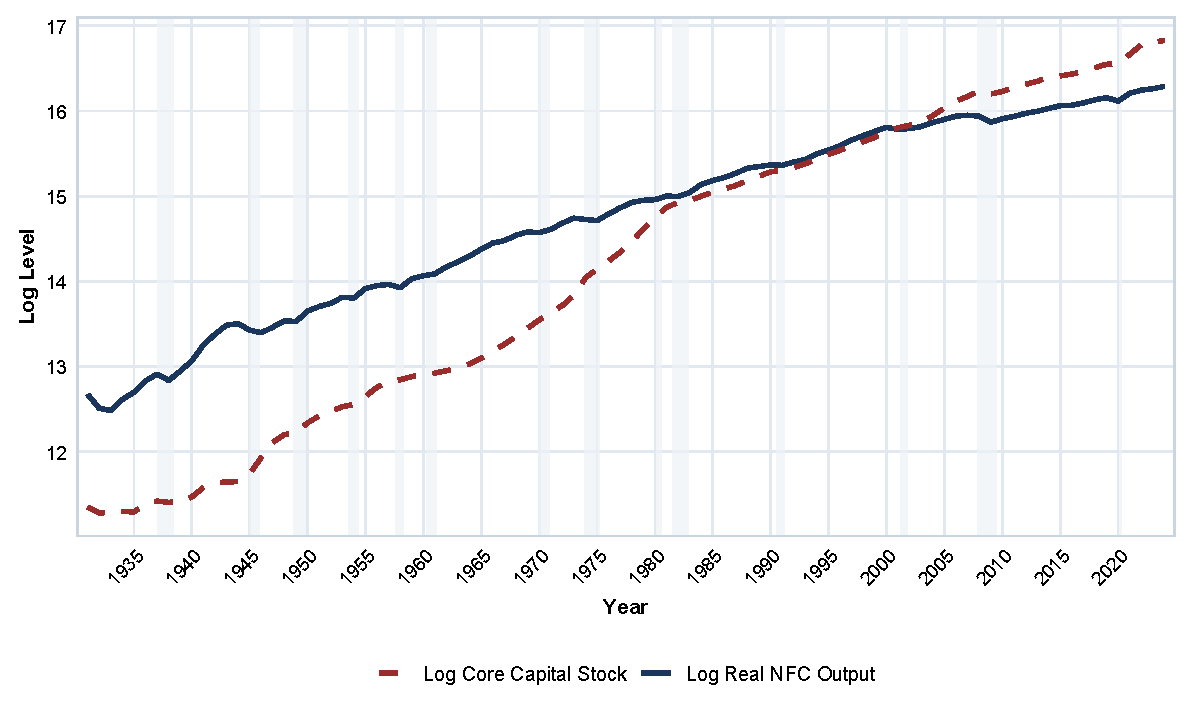
\includegraphics[scale=0.8]{figures/fig_us_stylized_1_y_kcap.pdf}
	\begin{tabular}{p{0.92\textwidth}}
		{\scriptsize \textbf{Note:} Log real non-financial corporate gross value added ($y_t$, solid navy line) and log core capital stock ($k_t^{cap} = \ln[K_t^{\text{ME}} + K_t^{\text{NRC}}]$, dashed crimson line). Light gray shaded bands denote official NBER recession dates.}
	\end{tabular}
\end{figure}

\begin{figure}[H]
	\centering
	\caption{U.S. Log Output--Capital Ratio ($y_t - k_t^{cap}$)}
	\label{fig:us_stylized_2_yk_ratio}
	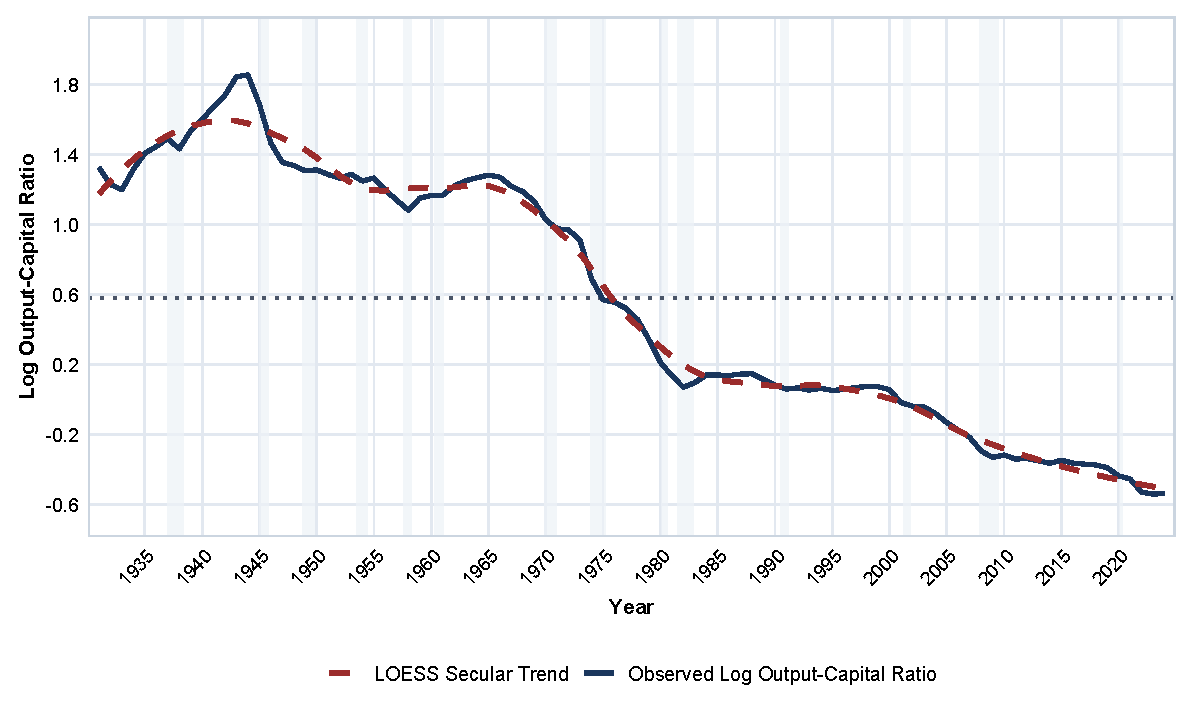
\includegraphics[scale=0.75]{figures/fig_us_stylized_2_yk_ratio.pdf}
	\begin{tabular}{p{0.92\textwidth}}
		{\footnotesize \textbf{Note:} Annual log difference of output and core capital stock ($y_t - k_t^{cap}$, solid navy line) relative to the full-sample mean (dotted line) and LOESS non-parametric secular trend (dashed crimson line, span = 0.35). Light gray background bands indicate NBER recessions.}
	\end{tabular}
	\vspace{2.5ex}
	\centering
	\caption{U.S. Capital Composition and Mechanization Gap ($\kappa_t = k_t^{\text{ME}} - k_t^{\text{NRC}}$)}
	\label{fig:us_stylized_2b_kappa}
	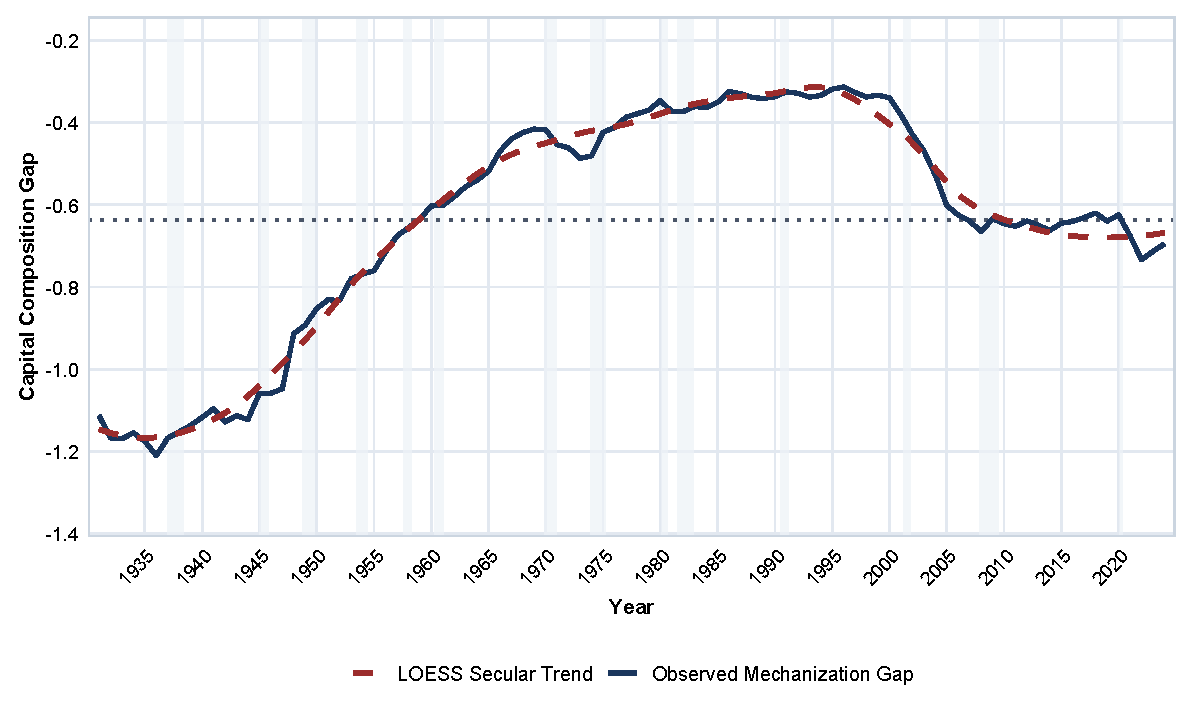
\includegraphics[scale=0.75]{figures/fig_us_stylized_2b_kappa.pdf}
	\begin{tabular}{p{0.92\textwidth}}
		{\scriptsize  \textbf{Note:} Non-financial corporate mechanization gap $\kappa_t = k_t^{\text{ME}} - k_t^{\text{NRC}}$ (solid navy line) relative to the full-sample mean ($-0.637$, dotted line) and LOESS non-parametric secular trend (dashed crimson line, span = 0.35). Light gray background bands indicate NBER recessions. Data sourced from BEA Fixed Assets Accounts.}
	\end{tabular}
\end{figure}

\begin{figure}[H]
	\centering
	\caption{U.S. Annual Growth Rates of Real Output and Core Capital Accumulation (1931--2024)}
	\label{fig:us_stylized_3_growth_rates}
	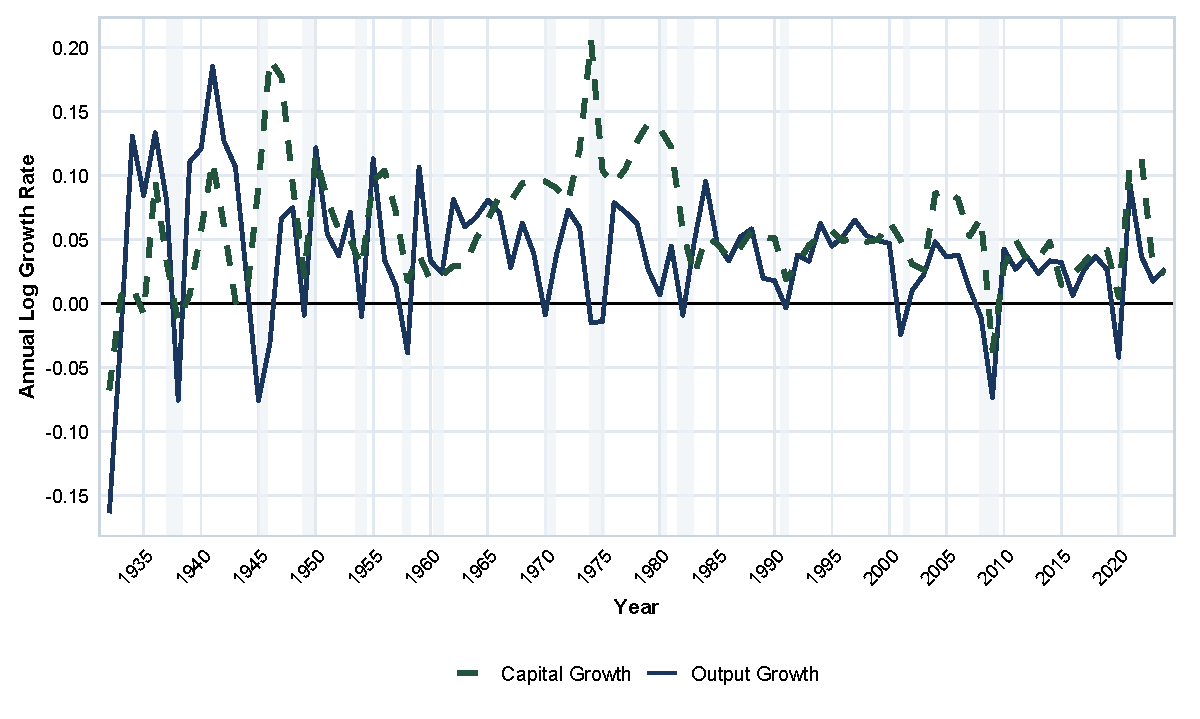
\includegraphics[scale=0.75]{figures/fig_us_stylized_3_growth_rates.pdf}
	\begin{tabular}{p{0.92\textwidth}}
		{\scriptsize \textbf{Note:} Annual growth rates of non-financial corporate real gross value added ($\Delta y_t$, solid navy line) and core physical capital stock ($\Delta k_t^{cap}$, dashed crimson line). Light gray background bands denote official NBER recession dates.}
	\end{tabular}
\end{figure}

\begin{figure}[H]
	\centering
	\caption{U.S. Wage Share Distributive Measures (1931--2024)}
	\label{fig:us_stylized_4a_distributive_state}
	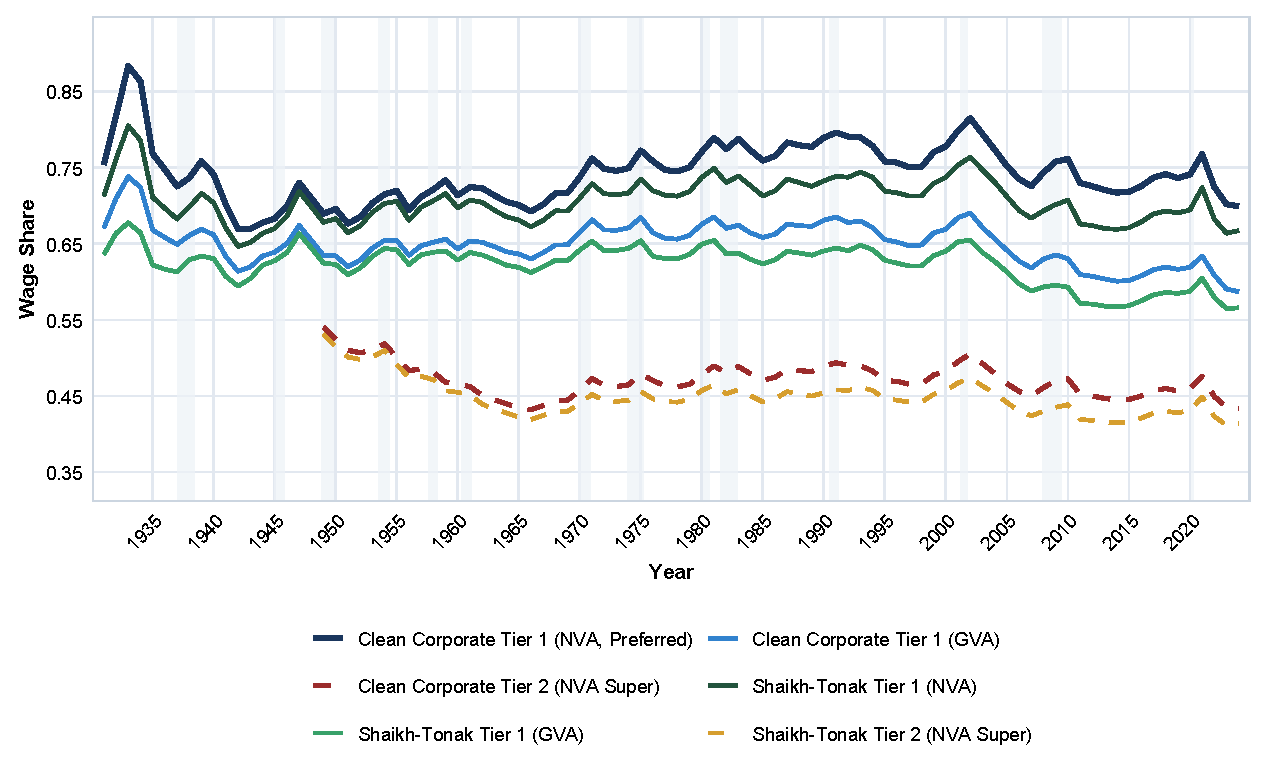
\includegraphics[scale=0.75]{figures/fig_us_stylized_4a_distributive_state.pdf}
	\begin{tabular}{p{0.95\textwidth}}
		{\scriptsize \textbf{Note:} Wage share permutations, value-added bases, and supervisory adjustments. Light gray background bands indicate NBER recessions.}
	\end{tabular}
	\vspace{2.5ex}
	\centering
	\caption{U.S. Effective Wage Pressure Measures (Scaled by IPP Capital Share, $C_t = \omega_{t-1}(1 - \iota_{t-1})$)}
	\label{fig:us_stylized_4b_distributive_state}
	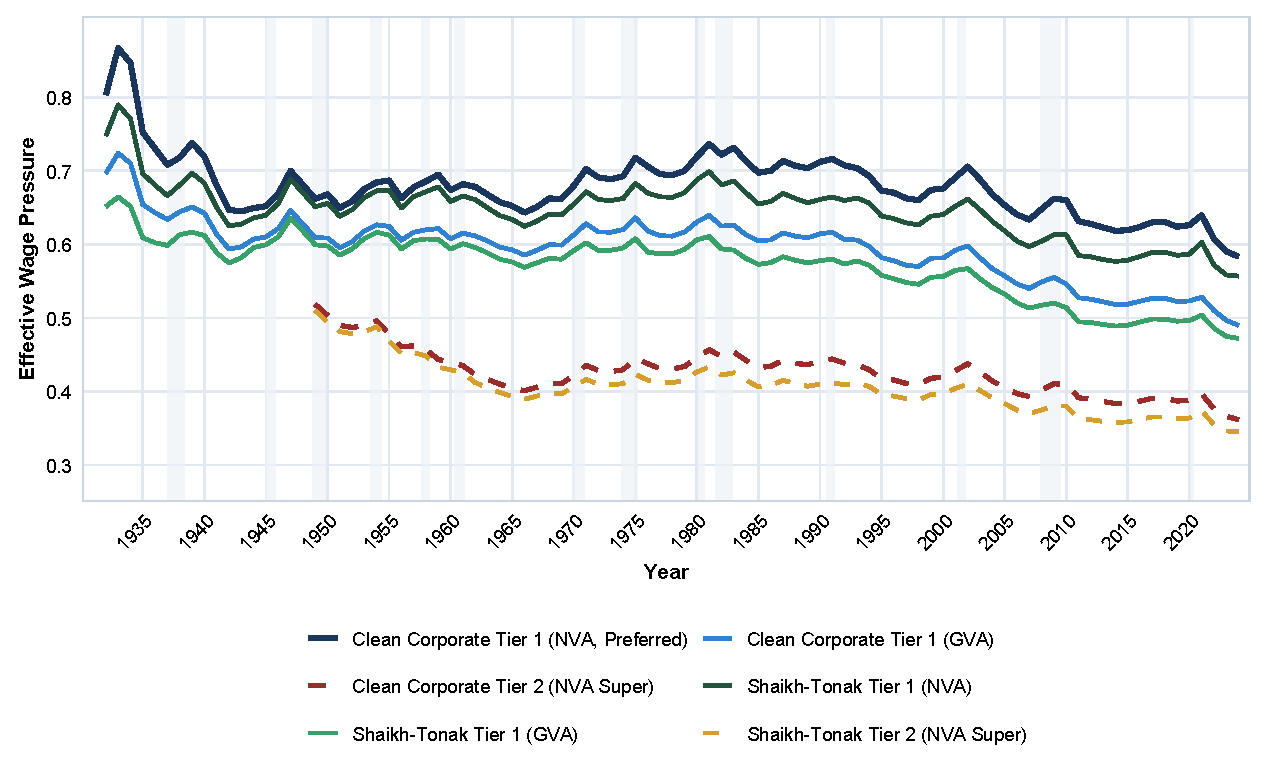
\includegraphics[scale=0.75]{figures/fig_us_stylized_4b_distributive_state.pdf}
	\begin{tabular}{p{0.95\textwidth}}
		{\scriptsize \textbf{Note:} Effective wage pressure permutations $C_t = \omega_{t-1}(1 - \iota_{t-1})$ Light gray background bands indicate NBER recessions.}
	\end{tabular}
\end{figure}


\pagebreak
\subsubsection{Stylized Facts of Peripheral Accumulation in Chile (1940--2010)}

Table~\ref{tab:cl_stylized_facts_summary} presents summary statistics for the core macroeconomic, distributive, and external variables of the Chilean economy over the 1940--2010 sample, capturing the long-run means and volatilities of real output, capital accumulation, income distribution, and the balance of payments. Because these aggregate moments obscure the pronounced historical regime shifts characteristic of the periphery, the series that follow trace the structural breaks, distributive fractures, and external constraint variables that motivate the heterogeneous-capital analytical framework presented in Section~3.3 and the threshold empirical strategy developed below.

\begin{table}[H]
\centering
\footnotesize
\caption{Chile Descriptive Statistics (1940--2010)}
\label{tab:cl_stylized_facts_summary}
\begin{tabular}{p{7.5cm} p{2.5cm} p{2.5cm}}
\hline\hline
\textbf{Variable} & \textbf{Mean} & \textbf{Std. Dev.} \\
\hline
Log Real GDP ($y_t$) & 16.625 & 0.776 \\
Log Core Capital Stock ($k_t^{cap}$) & 18.419 & 0.899 \\
Log Output--Capital Ratio ($y_t - k_t^{cap}$) & -1.793 & 0.169 \\
Capital Composition Gap ($\kappa_t$) & -1.106 & 0.211 \\
Gross Wage Share ($\omega_t^{gross}$) & 0.501 & 0.092 \\
Net Wage Share ($\omega_t^{net}$) & 0.802 & 0.121 \\
Central Bank Solvency Ratio ($S_t$) & 2.102 & 2.201 \\
Log Terms of Trade ($\ln \text{ToT}_t$) & 0.030 & 0.263 \\
Log Real Exports ($\ln X_{\text{FOB},t}$) & 14.753 & 1.116 \\
Log Machinery Investment ($\ln I_t^{\text{ME}}$) & 13.307 & 1.335 \\
\hline\hline
\multicolumn{3}{p{12.5cm}}{\scriptsize \textbf{Note:} Sample window spans 1940--2010 ($N = 71$). Real GDP and capital stock components sourced from Díaz, Lüders and Wagner (2016) and Pérez and Eyzaguirre (2021). Core capital stock is $K_t^{cap} = K_t^{\text{ME}} + K_t^{\text{NRC}}$. Capital composition gap $\kappa_t = k_t^{\text{ME}} - k_t^{\text{NRC}}$. Both Gross wage share (nominal compensation / nominal GDP) and Net wage share (nominal compensation / nominal NVA) are evaluated in nominal terms. Structural threshold $\hat{\gamma} = 0.425$ separates binding foreign exchange bottleneck regimes.} \\
\end{tabular}
\end{table}



Log real GDP ($y_t$) and aggregate gross core capital stock ($k_t^{cap} = \ln[K_t^{\text{ME}} + K_t^{\text{NRC}}]$) for Chile (1940--2010) are plotted on the same 2003 CLP price basis in Figure~\ref{fig:cl_stylized_1a_y_kcap}. Over seven decades, output and capital drift together along a shared upward trajectory, motivating the cointegrating specification. Dotted vertical lines mark the 1973 military coup and the 1990 post-dictatorship period.

The corresponding log output--capital ratio ($y_t - k_t^{cap}$) for Chile is plotted in Figure~\ref{fig:cl_stylized_1b_yk_ratio}. Unlike the continuous secular decline in the center, the peripheral output--capital ratio exhibits pronounced regime shifts: rising during the initial state-led ISI phase (1940--1955), collapsing during the 1972--1975 breakdown and the 1982 debt crisis, and settling into an unconstrained expansion during the 1990s commodity boom.

The mechanization gap $\kappa_t = k_t^{\text{ME}} - k_t^{\text{NRC}}$, plotted in Figure~\ref{fig:cl_stylized_2_kappa_mechanization} (mean $-1.106$, SD $0.211$, Table~\ref{tab:cl_stylized_facts_summary}), widens from the late 1940s through state-led ISI to 1972, stagnates under the early neoliberal regime with a debt-boom hump at 1981 and a post-crisis trough in the late 1980s, and rises sharply after redemocratization, when export-oriented mining pulled machinery accumulation ahead of structures. The gap is therefore a regime-shifting series rather than a smooth trend, which is what motivates the heterogeneous-capital specification in which $\theta$ depends on $\kappa_t$.

Figure~\ref{fig:cl_stylized_3_wage_share} documents the distributive side,
drawn from the revised real-wage dataset of \citet{Astorga2017, Astorga2023}
spliced with the national accounts. The gross wage share (mean 0.501, SD
0.092) peaks at $0.69$ in 1972 under Unidad Popular redistribution,
collapses to $0.40$ by 1975 after the military coup, recovers partially during the
debt boom that ends in 1982, and stabilizes under the post-dictatorship democratic
regime. The net wage share $\omega_t^{\text{net}} = \omega_t^{\text{gross}} / (1 - \text{CFC\_ratio\_nom}_t)$ (mean 0.768, SD 0.117, Table~\ref{tab:cl_stylized_facts_summary}) sits systematically above the gross share due to consumption of fixed capital; both series follow the same structural fractures. Two empirical facts matter for estimation: the 1972--1975 swing is the largest distributive shock in the sample, and the post-1990 wage-share stabilizes while the external accounts are mostly slack, which is what identifies the unconstrained mechanization response.

Figure~\ref{fig:cl_stylized_4_minipages} disaggregates the external
bottleneck into its components. The solvency ratio (Panel a), central bank
reserves relative to base money, is flat and low until 1975, jumps after the
debt crisis as the Bank accumulated reserves, and declines again after the
mid-2000s. The terms of trade (Panel b) deteriorate through the 1970s and
1980s and recover only with the commodity super-cycle. Real exports
(Panel c) grow smoothly, so the binding episodes are driven by reserve
solvency and import demand rather than by export failure; the import
imbalance series follows the World Historical Balance of Payments database
of \citet{NievasPiketty2025}. Machinery investment (Panel d) grows in bursts
separated by the crisis dates, consistent with mechanization that is
interrupted rather than smoothly accumulated. Section~4.5 assembles these
components into the composite index through a grid search, and estimates the threshold at which the external constraint becomes binding and counteracts the mechanization bias productivity gain. 


\begin{figure}[h!]
	\centering
	\caption{Chilean Log Real GDP and Aggregate Gross Core Capital Stock (1940--2010)}
	\label{fig:cl_stylized_1a_y_kcap}
	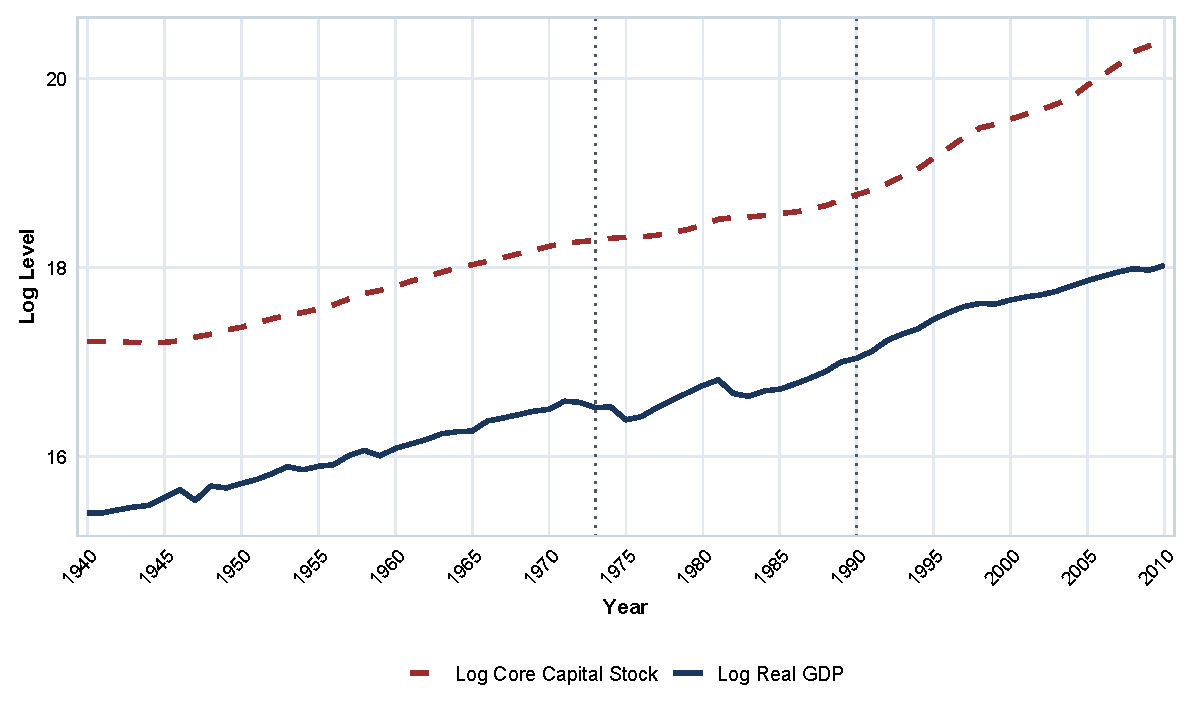
\includegraphics[scale=0.75]{figures/fig_cl_stylized_1a_y_kcap.pdf}
	\begin{tabular}{p{0.92\textwidth}}
	{\scriptsize \textbf{Note:} Log real GDP ($y_t$, solid navy line) and log aggregate gross core capital stock ($k_t^{cap} = \ln[K_t^{\text{ME}} + K_t^{\text{NRC}}]$, dashed crimson line). Vertical dotted lines mark 1973 (military coup) and 1990 (post-dictatorship).}
	\end{tabular}
\end{figure}

\begin{figure}[H]
	\centering
	\caption{Chile: Log Output--Capital Ratio ($y_t - k_t^{cap}$)}
	\label{fig:cl_stylized_1b_yk_ratio}
	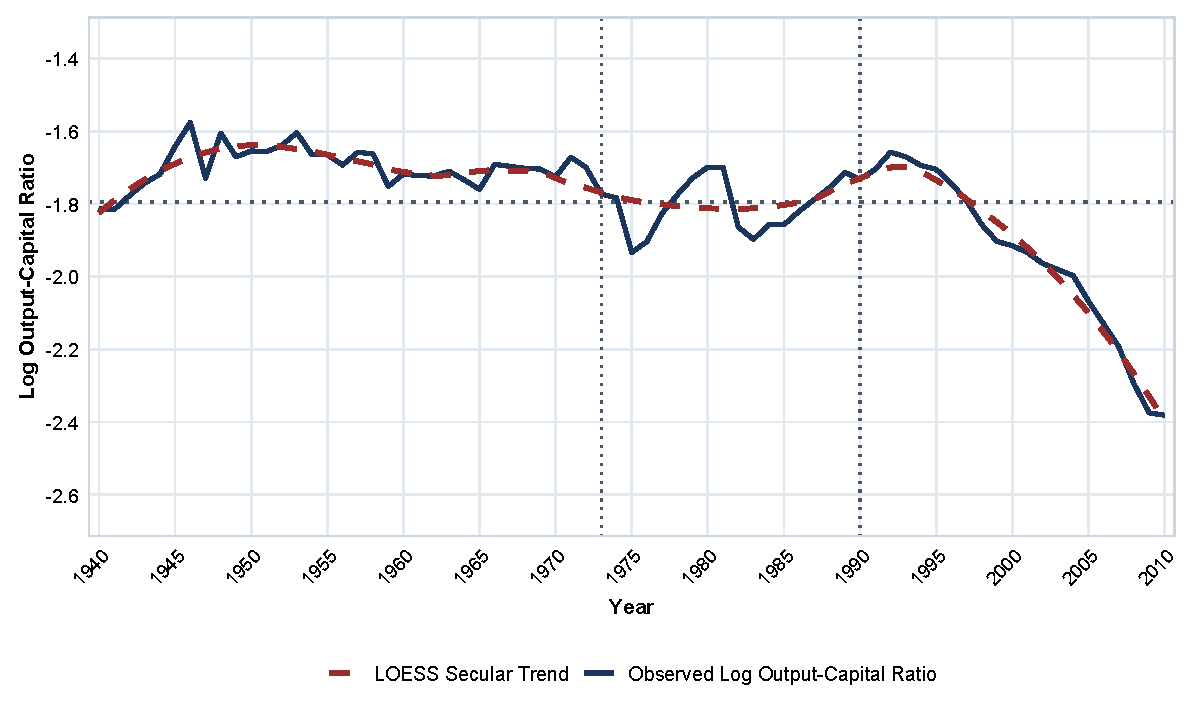
\includegraphics[scale=0.75]{figures/fig_cl_stylized_1b_yk_ratio.pdf}
	\begin{tabular}{p{0.88\textwidth}}
		{\scriptsize \textbf{Note:} Annual log output--capital ratio ($y_t - k_t^{cap}$, solid navy line) relative to the full-sample mean (dotted line) and LOESS non-parametric secular trend (dashed crimson line, span = 0.35). Vertical dotted lines mark 1973 and 1990.}
	\end{tabular}
	
\end{figure}

\begin{figure}[H]
	\centering
	% --- Top Figure: Capital Composition Gap ---
	\caption{Chilean Capital Composition and Mechanization Gap ($\kappa_t = k_t^{\text{ME}} - k_t^{\text{NRC}}$)}
	\label{fig:cl_stylized_2_kappa_mechanization}
	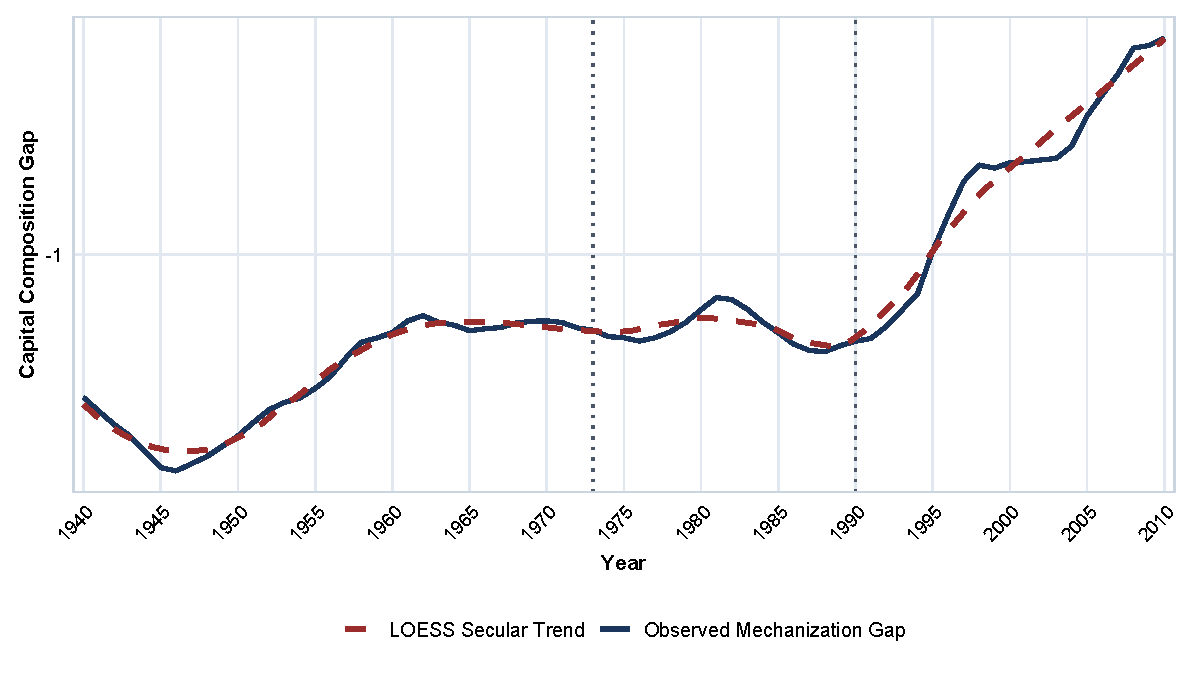
\includegraphics[scale=0.75]{figures/fig_cl_stylized_2_kappa_mechanization.pdf}
	\vspace{-0.5ex}
	\begin{tabular}{p{0.88\textwidth}}
		\scriptsize \textbf{Note:} Observed capital composition gap $\kappa_t = k_t^{\text{ME}} - k_t^{\text{NRC}}$ (solid navy line) alongside a LOESS non-parametric secular trend (dashed crimson line). Vertical dotted lines highlight the 1973 and 1990 political shifts.
	\end{tabular}
\end{figure}

	\vspace{1.5ex}

\begin{figure}[H]
	% --- Bottom Figure: Wage Share Trajectories ---
	\centering
	\caption{Chilean Wage Share Trajectories ($\omega_t^{\text{gross}}$ and $\omega_t^{\text{net}}$)}
	\label{fig:cl_stylized_3_wage_share}
	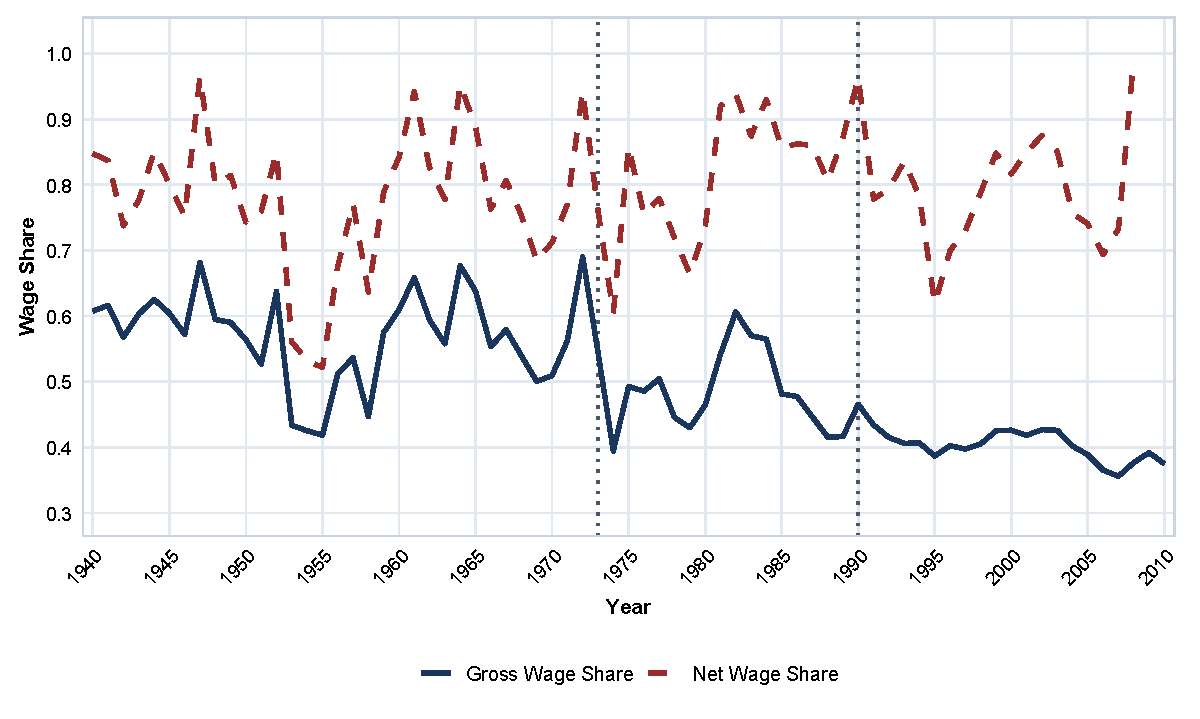
\includegraphics[width=0.88\textwidth, height=0.31\textheight, keepaspectratio]{figures/fig_cl_stylized_3_wage_share.pdf}
	\vspace{-0.5ex}
	\begin{tabular}{p{0.88\textwidth}}
		\scriptsize \textbf{Note:} Gross wage share $\omega_t^{\text{gross}}$ (solid navy line) and net wage share $\omega_t^{\text{net}}$ (dashed crimson line), 1940--2010. Vertical dotted lines highlight the 1973 and 1990 political shifts.
	\end{tabular}
	
	\vspace{2.5ex}

	\caption{Chilean External Bottleneck Constituent Series (1940--2010)}
	\label{fig:cl_stylized_4_minipages}
	\begin{minipage}{0.48\textwidth}
		\centering
		(a) Central Bank Solvency Ratio ($S_t$)\\
		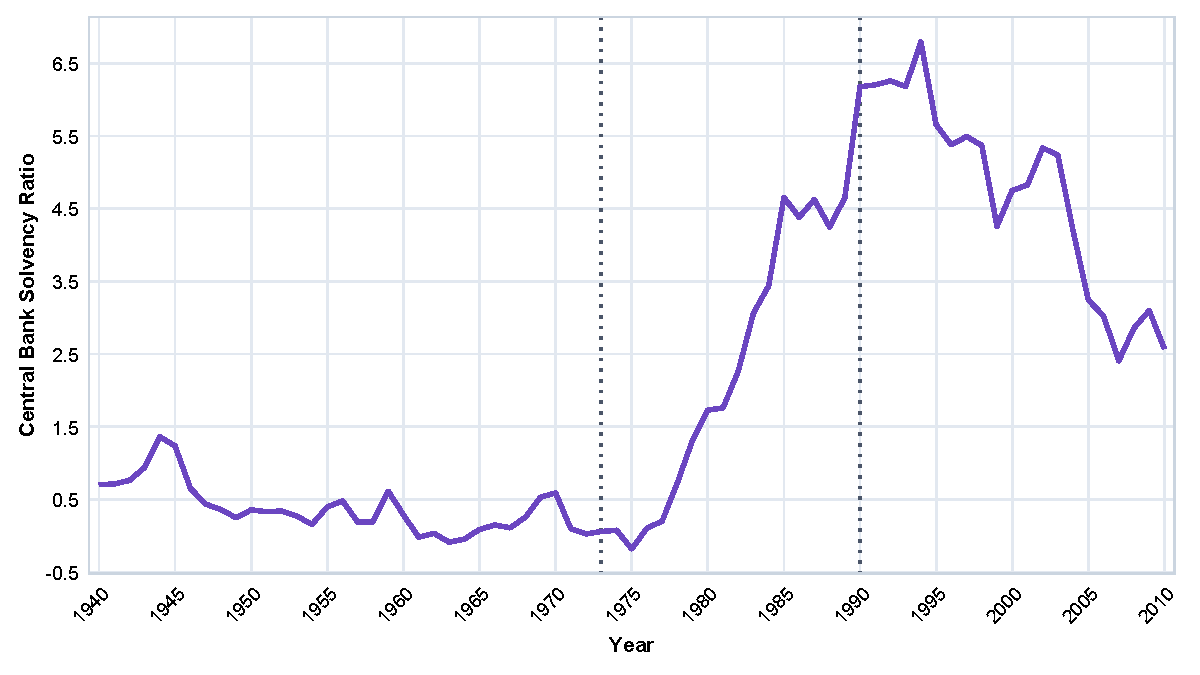
\includegraphics[width=\linewidth]{figures/fig_cl_stylized_4a_external_constraint.pdf}
	\end{minipage}\hfill
	\begin{minipage}{0.48\textwidth}
		\centering
		(b) Log Terms of Trade ($\ln \text{ToT}_t$)\\
		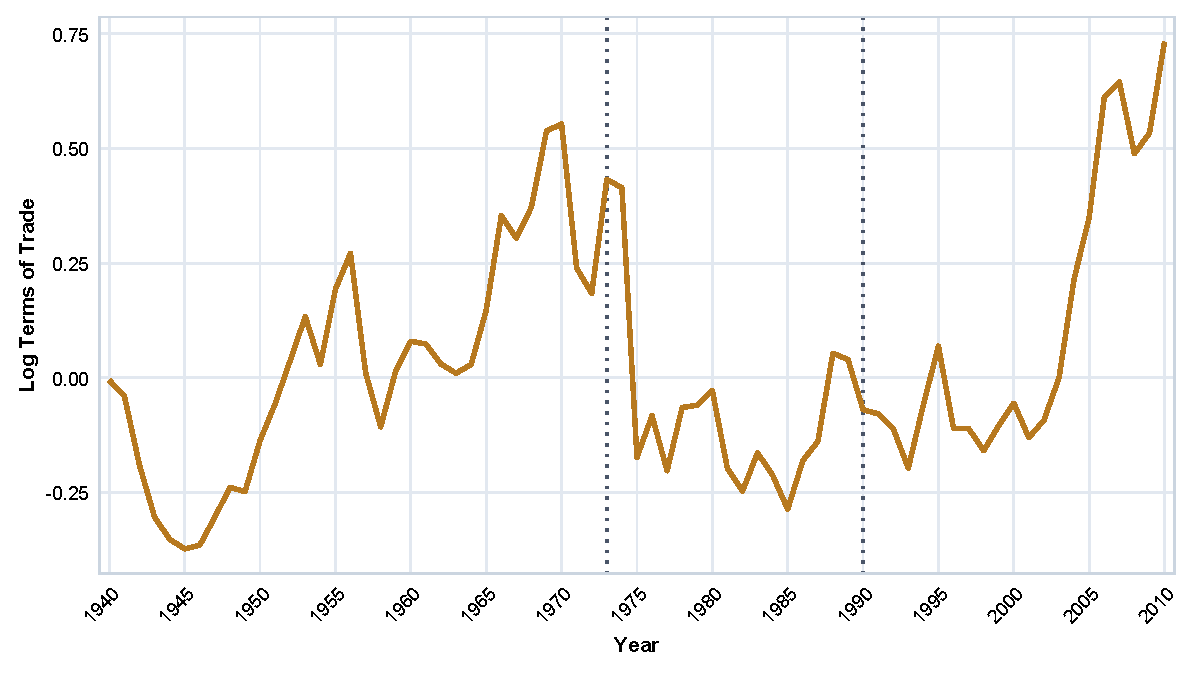
\includegraphics[width=\linewidth]{figures/fig_cl_stylized_4b_external_constraint.pdf}
	\end{minipage}
	
	\vspace{2ex}
	
	\begin{minipage}{0.48\textwidth}
		\centering
		(c) Log Real Exports ($\ln X_{\text{FOB},t}$)\\
		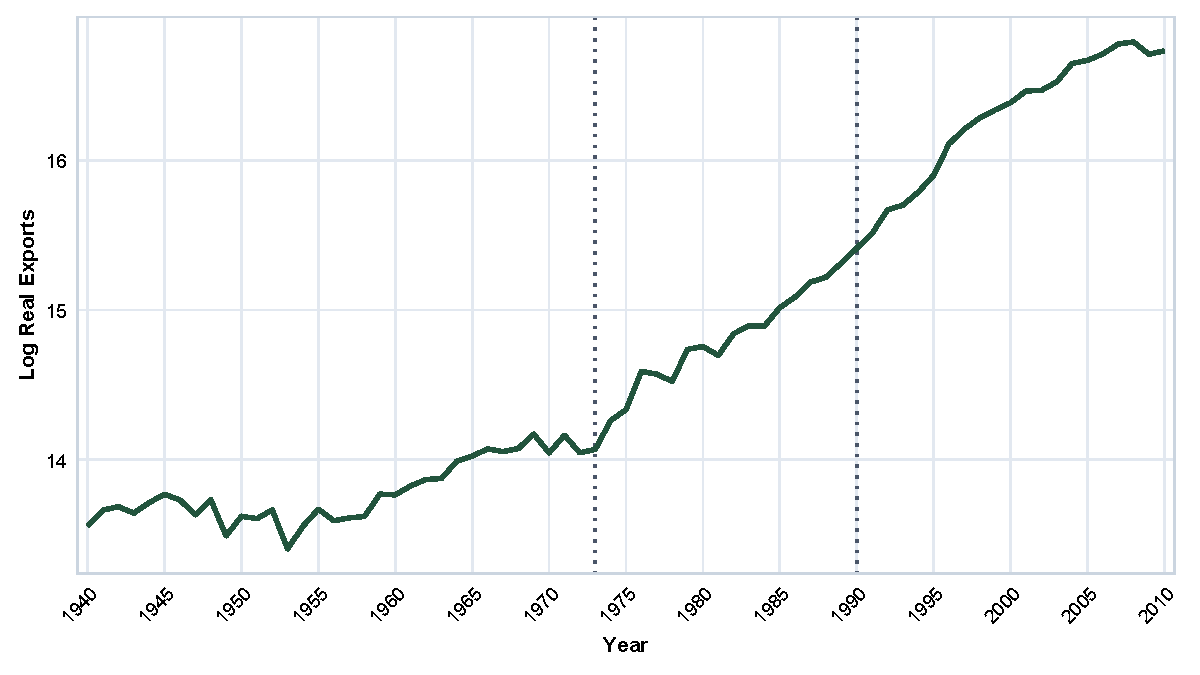
\includegraphics[width=\linewidth]{figures/fig_cl_stylized_4c_external_constraint.pdf}
	\end{minipage}\hfill
	\begin{minipage}{0.48\textwidth}
		\centering
		(d) Log Machinery Investment ($\ln I_t^{\text{ME}}$)\\
		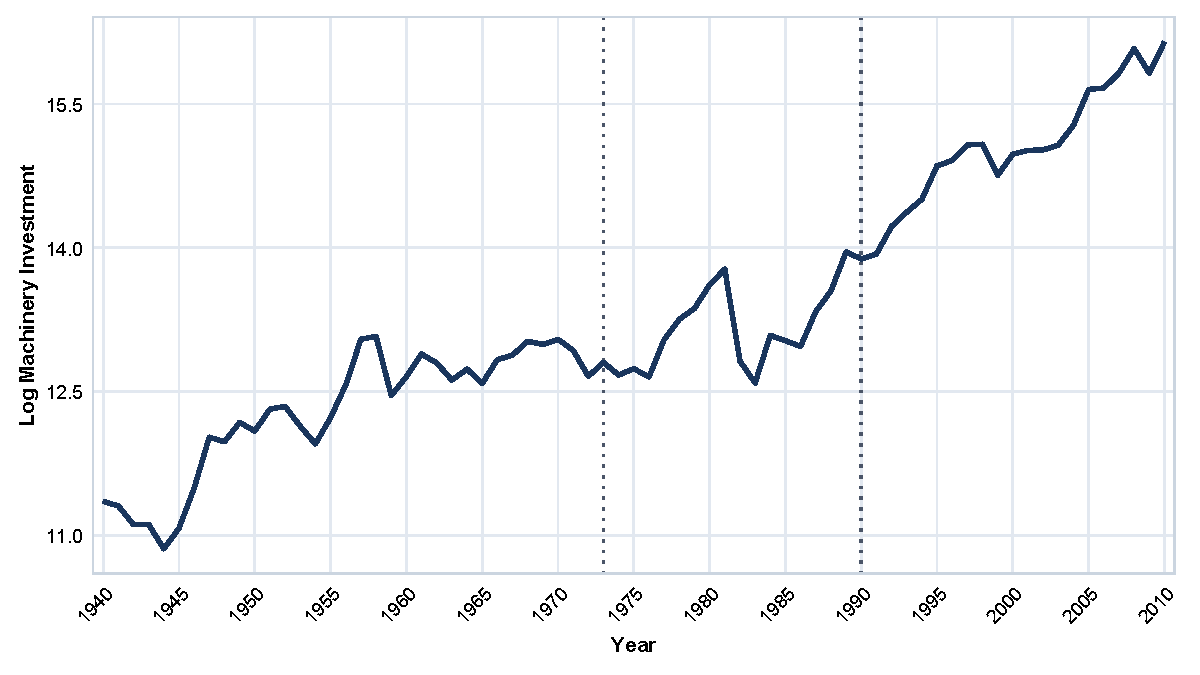
\includegraphics[width=\linewidth]{figures/fig_cl_stylized_4d_external_constraint.pdf}
	\end{minipage}
	\begin{flushleft}
	\begin{singlespace}\vspace{1ex}
		{\scriptsize \textbf{Note:} Disaggregated empirical constituent series to estimate the balance-of-payments constraint. Panel (a) plots Central Bank foreign exchange reserve solvency ($S_t$, international reserves expressed in domestic currency over monetary aggregates). Panels (b) and (c) plot the log terms of trade and log real exports, which together compose log real capital import purchasing power ($\ln M_t^{\text{cap,ToT}} = \ln \text{ToT}_t + \ln X_t$). Panel (d) plots active gross machinery investment demand ($\ln I_t^{\text{ME}}$). Vertical dotted lines mark 1973 and 1990.}
	\end{singlespace}
	\end{flushleft}
\end{figure}




%%%%%%%%%%%%%%%%%%%%%%%%%%%%%%%%%%%%%%%%%%%%%%%%%%%%%%%
%%%%% 4.3. Econometric Strategy IM-OLS Cointegration
%%%%%%%%%%%%%%%%%%%%%%%%%%%%%%%%%%%%%%%%%%%%%%%%%%%%%%%
\pagebreak
\subsection{Estimation Strategy: Cointegration and IM-OLS}
\label{sec:42:estimation_strategy}


\paragraph{The cointegrating regression.}
The transformation elasticity $\theta$ is estimated from the
cointegrating regression
\begin{equation}
	y_t = \alpha + \theta_0\, k_t
	+ \theta_1\, (k_t \times \omega_{t-1}) + u_t,
	\label{eq:421:coint_reg}
\end{equation}
where $y_t = \ln Y_t$ is log real output, $k_t = \ln K_t$ is log
real capital stock, and $\omega_{t-1}$ is the lagged wage share.
The regressors $k_t$ and $k_t \times \omega_{t-1}$ are integrated
of order one, and the error term $u_t$ is stationary under the null
hypothesis of cointegration. The interaction term
$k_t \times \omega_{t-1}$ is included in the regression to allow
the transformation elasticity to vary with the distributive state:
the effective elasticity is $\theta(\omega_{t-1}) = \theta_0
+ \theta_1\, \omega_{t-1}$.

\paragraph{The IM-OLS estimator.}
The OLS estimator of $\theta$ in \eqref{eq:421:coint_reg} is
super-consistent but its limiting distribution is contaminated by
second-order bias terms arising from endogeneity of the regressors
and serial correlation in the error term
\citep{PhillipsHansen1990}. The Integrated Modified OLS (IM-OLS)
estimator of \citet{VogelsangWagner2014} removes these bias terms
without requiring the choice of tuning parameters (kernel function,
bandwidth, or lead-lag truncation order) at the estimation stage.

The IM-OLS estimator is based on a two-step transformation. First,
the partial sum transformation is applied to
\eqref{eq:421:coint_reg}:
\begin{equation}
	S_{y,t} = S_{\alpha,t} + \theta_0\, S_{k,t}
	+ \theta_1\, S_{k\omega,t} + S_{u,t},
	\label{eq:421:partial_sum}
\end{equation}
where $S_{y,t} = \sum_{j=1}^{t} y_j$ and analogously for the
remaining terms. The partial sum transformation replaces the
cross-product terms $\sum_{t=1}^{T} x_t u_t$, whose limits contain
additive nuisance parameters, with partial-sum cross-products
$\sum_{t=1}^{T} S_{x,t}\, S_{u,t}$, whose limits do not. Second,
the partial-sum regression is augmented by the original regressors
$k_t$ and $k_t \times \omega_{t-1}$:
\begin{equation}
	S_{y,t} = S_{\alpha,t} + \theta_0\, S_{k,t}
	+ \theta_1\, S_{k\omega,t}
	+ k_t\, \gamma_1
	+ (k_t \times \omega_{t-1})\, \gamma_2
	+ S_{u,t}.
	\label{eq:421:imols_augmented}
\end{equation}
The augmentation absorbs the endogeneity correlation into the
coefficients $\gamma_1$ and $\gamma_2$, yielding a zero-mean
Gaussian mixture limiting distribution for the IM-OLS estimator of
$(\theta_0, \theta_1)$ conditional on the Brownian motions driving
the regressors \citep[Theorem 2]{VogelsangWagner2014}.

\paragraph{FWL orthogonalization of the interaction term.}
The interaction term $k_t \times \omega_{t-1}$ is correlated with
$k_t$ by construction. To isolate the distributive mediation effect,
the interaction term is orthogonalized against $k_t$ and the
deterministic regressors using the Frisch-Waugh-Lovell (FWL)
theorem \citep{FrischWaugh1933,Lovell1963}. Denoting the raw interaction by
$\xi_t = k_t \times \omega_{t-1}$, the orthogonalized interaction
$\xi_t^{\perp}$ is the residual from the auxiliary regression of
$\xi_t$ on $k_t$ and the deterministic regressors. The IM-OLS
estimator is then applied to the regression with $\xi_t^{\perp}$
replacing $\xi_t$. When structural break dummies are included in
the deterministic regressors (see below), the FWL orthogonalization
is re-computed against the augmented deterministic space.

\paragraph{Endogenous structural break detection.}
The estimation employs a two-pass endogenous break detection
procedure based on \citet{BaiPerron2003}. In the first pass, the
IM-OLS estimator is applied to \eqref{eq:421:coint_reg} without
break dummies. The Bai-Perron sequential procedure is then applied
to the IM-OLS residuals to detect structural breaks at unknown
dates, with a minimum segment size of 15\% of the sample. In the
second pass, step dummies $D_t^{(b)} = \mathbf{1}\{t \geq
\hat{T}_b\}$ are included in the deterministic regressors for each
detected break date $\hat{T}_b$, the FWL orthogonalization is
re-computed, and the IM-OLS estimator is re-estimated.

\paragraph{Fixed-$b$ inference.}
Standard asymptotic theory treats the bandwidth $M$ in long-run
variance estimation as vanishing relative to the sample size
($M/T \to 0$). Under this assumption, the long-run variance
estimator converges to a constant, and $t$- and Wald statistics
are compared to normal or chi-squared critical values. In finite
samples with serially correlated errors and endogenous regressors,
however, the bandwidth choice materially affects the sampling
distribution of test statistics, and the standard approximation
over-rejects \citep{KieferVogelsang2005}. Fixed-$b$ asymptotic
theory addresses this by treating the bandwidth ratio
$b \equiv M/T$ as a fixed constant rather than a vanishing
sequence. The long-run variance estimator then converges not to a
constant but to a random variable whose distribution depends on
the kernel function, the bandwidth ratio $b$, the number of
integrated regressors, and the deterministic specification.
Critical values that reflect these choices can be tabulated by
simulation, and using them substantially reduces size distortions
at the cost of only minor losses in power
\citep{VogelsangWagner2014}.

For testing $q$ linear restrictions $H_0: R\theta = r$, the
fixed-$b$ Wald statistic is
\begin{equation}
	W^{*} = (R\tilde{\theta} - r)'
	\bigl[R\, A_{\text{IM}}\, \tilde{V}_{\text{IM}}\,
	A_{\text{IM}}'\, R'\bigr]^{-1}
	(R\tilde{\theta} - r),
	\label{eq:421:fixedb_wald_stat}
\end{equation}
where $\tilde{V}_{\text{IM}}$ is the IM-OLS covariance estimator
constructed from the adjusted residuals
$\Delta\tilde{S}^{u*}_t$ (defined below). Under fixed-$b$
asymptotics, $W^{*}$ converges to
\begin{equation}
	W^{*} \Rightarrow \frac{\chi^2_q}{Q_b(\tilde{P}^{*},
		\tilde{P}^{*})},
	\label{eq:421:fixedb_wald}
\end{equation}
where $\chi^2_q$ is a chi-squared random variable with $q$
degrees of freedom---one per restriction tested---and
$Q_b(\tilde{P}^{*}, \tilde{P}^{*})$ is a positive random
variable that captures the effect of the bandwidth and kernel
choices on the long-run variance estimator. The two quantities
in \eqref{eq:421:fixedb_wald} are independent of each other
\citep[Lemma 2, Proposition 3]{VogelsangWagner2014}. This
independence is the operative property: it renders the limiting
distribution of $W^{*}$ free of unknown nuisance parameters, so
that critical values depend only on the known features of the
specification---the kernel, the bandwidth ratio $b$, the number
of integrated regressors, and the deterministic components---and
can be tabulated by simulation. Critical values for the Bartlett
kernel with intercept-only deterministics and up to four
integrated regressors are provided in the online supplement to
\citet{VogelsangWagner2014}. Because the fixed-$b$ distribution is
jointly indexed by the bandwidth ratio and the number of integrated
regressors, no single tabulated constant applies across the
specifications estimated here; the significance thresholds reported
in every results table are therefore obtained by direct Monte Carlo
simulation of the exact data-generating process under test.
Appendix~\ref{app:critical_values} collects the fixed critical
values used for the residual-based diagnostics and states the
simulation protocol for the fixed-$b$ Wald statistics.

The adjusted residuals $\Delta\tilde{S}^{u*}_t$ used for
long-run variance estimation are obtained in two steps. First,
the IM-OLS residuals $\tilde{S}_{u,t}$ from
\eqref{eq:421:imols_augmented} are correlated with the IM-OLS
estimator $\tilde{\theta}$ even asymptotically, because the
partial-sum regression contains integrated regressors. This
correlation prevents the residuals from being used directly
for fixed-$b$ inference. Second, to remove this correlation,
$\tilde{S}_{u,t}$ is projected on a set of constructed
regressors $H_t^{\perp}$ (functions of the partial sums of the
deterministic components and the integrated regressors), yielding
\begin{equation}
	\Delta\tilde{S}^{u*}_t = \Delta\tilde{S}_{u,t}
	- \Delta H_t^{\perp\,\prime}\,\hat{\varrho},
	\label{eq:421:adjusted_residuals}
\end{equation}
where $\hat{\varrho}$ is the OLS coefficient vector from the
regression of $\tilde{S}_{u,t}$ on $H_t^{\perp}$. The resulting
adjusted residuals are asymptotically independent of
$\tilde{\theta}$, which is the condition required for the
numerator and denominator in \eqref{eq:421:fixedb_wald} to be
independent and for the critical values to be pivotal.

\paragraph{Cointegration testing.}
Two complementary tests are employed to assess the presence of a
cointegrating relationship. First, the null hypothesis of
cointegration is tested using a \citet{Shin1994} type KPSS statistic
applied to the IM-OLS residuals \citep{WagnerHong2016,Wagner2023}:
\begin{equation}
	C_T = \frac{1}{T^2\, \hat{\omega}_{u \cdot v}^2}
	\sum_{t=1}^{T}
	\left(\sum_{j=1}^{t} \hat{u}_j
	\right)^2,
	\label{eq:421:shin_ct}
\end{equation}
where $\hat{\omega}_{u \cdot v}^2$ is a consistent estimator of
the conditional long-run variance $\omega_{u \cdot v}^2
= \Omega_{uu} - \Omega_{uv}\Omega_{vv}^{-1}\Omega_{vu}$. Under
the null hypothesis of cointegration, $C_T$ converges to a
functional of standard Brownian motions whose critical values depend
on the number of integrated regressors included in the regression
and the deterministic specification \citep{Wagner2013,Wagner2023}. Second,
the null hypothesis of no cointegration (spurious regression) is
tested using the augmented Dickey-Fuller statistic applied to the
OLS residuals with MacKinnon \citeyearpar{MacKinnon2010} finite-sample
critical values, with the lag order selected by the Akaike
information criterion. Rejection of the null hypothesis of no
cointegration combined with non-rejection of the null hypothesis of
cointegration constitutes evidence for a cointegrating relationship.

\subsubsection{Integration Order and Stochastic Properties: United States}
\label{sec:43:integration_order_us}

\paragraph{A}
In Cointegrating Multivariate Polynomial Regressions (CMPR) estimated via Integrated Modified OLS (IM-OLS) \citep{VogelsangWagner2014,VogelsangWagner2024}, valid asymptotic inference and pivotal fixed-$b$ Wald distributions require all stochastic regressors to be integrated of order one ($I(1)$). When non-linear interaction terms ($k_t \times \omega_{t-1}$, $k_t \times \omega_{t-1} \times (1-\iota_{t-1})$) enter the long-run relation, establishing their stochastic integration order prior to estimation is an essential prerequisite. We evaluate the stochastic properties of U.S. series and their interactions over 1929--2024 ($T = 96$) using Augmented Dickey-Fuller (ADF), DF-GLS, Phillips-Perron (PP), Kwiatkowski-Phillips-Schmidt-Shin (KPSS), and Zivot-Andrews (ZA) tests with endogenous structural breaks. The results confirm that log real output ($y_t$), core private gross capital ($k^{\text{cap}}$), the corporate Intellectual Property Products (IPP) gross investment share ($\iota_t$), and distributive wage shares ($\omega_i$) are clean $I(1)$ processes (rejecting level stationarity at $p < 0.01$ under KPSS, and rejecting unit roots in first differences at $p < 0.01$ under ADF and DF-GLS).

\paragraph{B}
A central property concerns the capital composition ratio ($\kappa_t = k^{\text{ME}}_t - k^{\text{NRC}}_t$). Both Machinery ($k^{\text{ME}}_t$) and Structures ($k^{\text{NRC}}_t$) are established $I(1)$ series. When evaluated in first differences under a standard linear KPSS specification, $\Delta \kappa_t$ displays apparent persistence ($KPSS_{\text{diff}} = 0.761, p < 0.01$). This reflects the sharp post-1973 structural deceleration in mechanization (identified by the 1974 Zivot-Andrews break) rather than an $I(2)$ process (Perron, 1989). When $\kappa_t$ and capital stocks are interacted with distributive wage shares and corporate IPP investment shares ($\iota_t \times \omega_i$, $\kappa_t \times \iota_t \times \omega_i$, $k^{\text{cap}} \times \omega_i$, $k^{\text{cap}} \times \omega_i \times \iota_t$), the bounded support of the wage and investment shares dampens the drift. All double and triple interaction terms are strictly $I(1)$ ($ADF_{\text{diff}} < -6.89, p < 0.01; KPSS_{\text{diff}} < 0.23$, failing to reject differenced stationarity), authorizing their inclusion in CMPR IM-OLS specifications.

\paragraph{C}
The Zivot-Andrews endogenous structural break tests identify transition dates that track the institutional history of U.S. capital accumulation:
\begin{enumerate}
	\item \textbf{1972 / 1974:} Capital stocks ($k^{\text{cap}}$) and capital composition ($\kappa_t$) break endogenously in 1972--1974 ($t_{\text{ZA}} = -4.79$ and $-3.63$), marking the exhaustion of the post-WWII Fordist accumulation boom.
	\item \textbf{1976:} Corporate IPP investment share ($\iota_t$) breaks in 1976 ($t_{\text{ZA}} = -4.53$), capturing the stagflation inflection toward intangible investments.
	\item \textbf{1984:} All eight IPP-wage interactions ($\iota_t \times \omega_i$) and triple interactions break strictly in 1984 ($t_{\text{ZA}} = -4.54$ to $-4.92$), reflecting the consolidation of the neoliberal regime under Reagan-Volcker through wage suppression and accelerated financialization.
	\item \textbf{2001--2003:} Capital-wage interactions ($k^{\text{cap}} \times \omega_i$) shift endogenously in 2001--2003 ($t_{\text{ZA}} = -4.26$ to $-4.85$), reflecting post-dot-com labor market restructuring.
\end{enumerate}

\paragraph{D}
The complete unit-root test batteries, test statistics, and critical values across all U.S. series and interaction terms are documented in Tables~\ref{tab:urca_results_ipp}--\ref{tab:urca_results_kcap} of Appendix~\ref{app:integration_order}.

\subsubsection{Integration Order and Stochastic Properties: Chile}
\label{sec:43:integration_order_cl}

\paragraph{A}
For the Chilean peripheral economy, the long-run estimation window spans 1943--2010 ($T = 68$). The 1943 start date isolates a stable institutional regime established by Law No.~7,200 (1942), which abandoned gold-standard convertibility and oriented Central Bank credit toward state-led import substitution alongside CORFO. Historical ClioLab external constraint and terms-of-trade series end in 2010. Unit-root tests over this horizon confirm that aggregate real GDP ($y_t$), Nonresidential Structures ($k^{\text{NR}}_t$), Machinery and Equipment ($k^{\text{ME}}_t$), aggregate core capital ($k^{\text{cap}}_t$), and distributive wage shares ($\omega^{\text{net}}_t, \omega^{\text{gross}}_t$) are $I(1)$ non-stationary processes.

\paragraph{B}
The composite Balance-of-Payments index ($Z_t = 0.2 \tilde{M}_t + 0.8 \tilde{S}_t$), which combines the normalized import coverage ratio and terms of trade, rejects the unit root null in levels ($ADF = -6.661, p < 0.01; KPSS = 0.075$). It operates as a stationary threshold state variable that partitions accumulation regimes. Furthermore, while raw nonresidential structures ($k^{\text{NR}}_t$) display moderate differenced persistence, FWL-orthogonalized wage interaction residuals ($\xi^{\omega}_t$) and the threshold-conditioned mechanization regressor ($k_t \times \omega_{t-1} \times \mathbf{1}\{Z_t \le 0.425\}$) are strictly $I(1)$ ($ADF_{\text{diff}} < -10.10, p < 0.01; KPSS_{\text{diff}} < 0.06$), satisfying the stochastic admissibility criteria for threshold CMPR estimation.

\paragraph{C}
The complete unit-root test batteries, test statistics, and critical values across all Chilean series and interaction terms are documented in Tables~\ref{tab:chile_urca_macro}--\ref{tab:chile_urca_interactions} of Appendix~\ref{app:integration_order}.


%%%%%%%%%%%%%%%%%%%%%%%%%%%%%%%%%%%%%%%%%%%%%%%%%
%%%%% 4.4. US Results Aggregate Capital
%%%%%%%%%%%%%%%%%%%%%%%%%%%%%%%%%%%%%%%%%%%%%%%%%


\subsection{United States: Baseline Specification Empirical Results}
\label{sec:431:specA_results}

\subsubsection{Baseline Econometric Specification}
I evaluate the empirical relationship between real aggregate output ($y_t = \log Y_{\text{REAL},t}^{\text{NFC}}$) and core physical productive capital stock ($k_{\text{cap},t} = \log(K_{\text{ME},t} + K_{\text{NRC},t})$) for the nonfinancial corporate business sector over the 1929--2024 period. Under Specification A, the aggregate cointegrating equation takes the form:
\begin{equation}
	y_t = \alpha + \theta_0\, k_{\text{cap},t} + \theta_1\, \xi^{\omega}_t + \boldsymbol{\gamma}' \mathbf{D}_t + u_t,
	\label{eq:431:specA_model}
\end{equation}
where $\xi^{\omega}_t$ denotes the Frisch-Waugh-Lovell (FWL) orthogonalized wage-capital interaction term, and $\mathbf{D}_t$ contains step-shift dummies capturing historical structural breaks identified via Bai-Perron tests. The FWL orthogonalization partials out base capital regressors and deterministic step shifts prior to estimating the interaction elasticity $\theta_1$, eliminating collinearity bias while preserving exact parameter identification \citep{VogelsangWagner2024}. Two distinct interaction sets are estimated across 48 total model permutations: Set 1 incorporates the standard unconditioned wage interaction $\xi^{\omega}_t = \omega_{t-1} \times k_{\text{cap},t}$, whereas Set 2 incorporates the effective wage pressure interaction $\xi^{\omega}_t = \omega_{t-1}(1 - \iota_{t-1}) \times k_{\text{cap},t}$, where $\iota_{t-1}$ represents the lagged share of intellectual property products in total capital stock. All parameters are estimated via Cointegrating Multivariate Polynomial Regression (CMPR) IM-OLS \citep{VogelsangWagner2024}, with non-standard fixed-$b$ critical values generated from a 100,000-pass Monte Carlo simulation suite matching the exact sample sizes ($T = 94$ for 1931--2024 standard series; $T = 77$ for 1948--2024 supervisory-adjusted series). Because capital stocks are constructed via Perpetual Inventory (GPIM) methods, classical right-hand-side measurement noise in $k_{\text{cap},t}$ introduces standard attenuation bias that pulls $\hat{\theta}_0$ downward toward zero, reinforcing that the structural transformation elasticity is bounded strictly below unity rather than an artifact of measurement error.

\paragraph{Theoretical argument for the NVA basis of distributive conflict measure.}
Class struggle over distribution is conducted strictly over newly created value ($\text{Net Value Added} = v + s$), excluding pre-existing constant capital transfers ($\text{Consumption of Fixed Capital} = \text{CFC}$). Under classical-Marxian national accounting \citep{ShaikhTonak1994}, $\text{Gross Value Added} = \text{CFC} + v + s$. Because physical depreciation ($\text{CFC}$) represents constant capital transferred to output by concrete labor, it lies outside zero-sum distributive conflict; rising $\text{CFC}/\text{GVA}$ during intensive mechanization mechanically depresses GVA wage shares even when the rate of surplus-value extraction ($s/v$) is invariant. The NVA basis ($\omega_{\text{NVA}} = v / (v + s)$) purges this physical depreciation distortion, isolating the balance of class power. Standard NIPA compensation includes managerial and executive salaries, which function as distributions of surplus value rather than variable labor costs. The Shaikh-Tonak Tier 2 ($\omega_{\text{ST,Tier2}} = v_{\text{prod}} / \text{NFC\_NVA}$) and Clean Corporate Tier 1 and Tier 2 measures strip supervisory overhead ($s_{\text{sup}}$) and purge financial sector double-counting ($\text{FIN\_NOS}^{\text{implied}} + \text{NFC\_NET\_INT}$), recovering the variable capital ($v$) that drives corporate cost-minimization decisions. Because unadjusted Shaikh-Tonak Tier 1 NVA ($\text{NFC\_COMP} / \text{NFC\_NVA}$) is mathematically identical to the NFC Baseline NVA share, Clean Corporate and Tier 2 supervisory adjustments constitute the primary non-redundant distributive specifications.

\paragraph{Institutional and physical mechanism of scaling by $(1-\iota_{t-1})$.}
The scaling factor $(1-\iota_{t-1}) = K_{\text{cap},t-1} / (K_{\text{cap},t-1} + K_{\text{IPP},t-1})$ isolates the physical productive asset share (machinery, equipment, and structures) from total fixed capital. Under the induced mechanization mechanism, when labor commands a larger share of newly created value ($\omega_{t-1} \uparrow$), squeezed profit margins compel firms toward defensive mechanization, substituting capital equipment for living labor on the shop floor. However, capital expenditure allocated to Intellectual Property Products ($K_{\text{IPP}}$)---software licenses, corporate patents, brand architecture, and legal protections---operates as market enclosure rather than physical output-yielding machinery. If investment shifts toward intangibles ($\iota \uparrow$), those funds bypass shop-floor labor substitution. In the Fordist era ($1931$--$1973$), IPP capital was negligible ($\iota \approx 0.02$--$0.05 \implies 1-\iota \approx 0.95$), allowing raw wage pressure to translate directly into physical machinery expansion. In the digital Post-Fordist era ($1980$--$2024$), IPP capital surged ($\iota > 0.28 \implies 1-\iota < 0.72$), diverting substantial surplus into software and legal enclosures. Unadjusted wage interactions ($\omega_{t-1} \times k_{\text{cap}}$ in Set 1) fail across the full sample because they assume an identical physical capacity yield across regimes; scaling by $(1-\iota_{t-1})$ purges this intangible diversion, capturing the effective wage pressure that drives shop-floor labor substitution.

\paragraph{Cointegration verdict across the test triad.}
Cointegration in Specification A is evaluated across three complementary tests: the Engle-Granger residual ADF test ($t_{\text{ADF}}$), the Shin \citeyearpar{Shin1994} LM test ($C_{\text{Shin}}$), and the Vogelsang-Wagner Type 2 Wald statistic ($S_{\text{Type 2}}$). Across all 48 specifications, the Shin LM test ($C_{\text{Shin}} \le 0.04$, $p > 0.10$) and the Vogelsang-Wagner Type 2 Wald statistic ($S_{\text{Type 2}} \le 13.18$, well below the 90th percentile fixed-$b$ critical value threshold of $52.6$) fail to reject the null hypothesis of cointegration ($H_0: \text{Cointegration}$). When Bai-Perron step shifts are included, the Engle-Granger residual ADF test rejects the null hypothesis of no cointegration ($t_{\text{ADF}} = -4.07$, $p < 0.05$ in Column 4), establishing that aggregate real output and private core capital form a genuine, non-spurious long-run cointegrating relationship.

\paragraph{Set 1 results: failure of standard unadjusted wage interactions.}
The Set 1 estimation results in Tables~\ref{tab:specA_set1_gva_app} and \ref{tab:specA_set1_nva_app} (Appendix~\ref{app:specA_full_results}) reveal two key patterns. First, the baseline capital transformation elasticity $\hat{\theta}_0$ is positive, highly stable, and statistically significant across all specifications ($0.55$--$0.61$, $p < 0.01$), establishing that private core capital ($K_{\text{cap}} = K_{\text{ME}} + K_{\text{NRC}}$) yields a long-run output elasticity of approximately $0.58$. Second, the unadjusted standard wage interaction $\hat{\theta}_1$ fails to achieve statistical significance in every Set 1 model, with point estimates ranging from $-0.02$ ($t = -0.16$) in NFC Baseline GVA/NVA to $-0.20$ ($t = -1.95$) in Clean Corporate Tier 2 NVA. Unconditioned wage shares fail to capture the induced accumulation channel because raw wage measures conflate unproductive managerial overhead with productive variable labor and ignore the structural allocation of investment toward intellectual property products.

\paragraph{Set 2 results: effective wage pressure and defensive mechanization.}
Table~\ref{tab:specA_set2_nva_main} presents the main-text Set 2 estimates for the Net Value Added basis, where wage pressure is scaled by productive capital accumulation $(1 - \iota_{t-1})$. When distributive conflict is evaluated over newly created net value and purged of supervisory overhead, effective wage pressure generates a statistically significant negative interaction elasticity $\hat{\theta}_1$. In the Clean Corporate Tier 1 NVA model with break shifts (Column 4), $\hat{\theta}_1 = -0.30$ ($t = -5.00$, $p < 0.05$). In the Clean Corporate Tier 2 NVA specification (Column 6), the coefficient reaches $\hat{\theta}_1 = -0.49$ ($t = -3.77$, $p < 0.05$), while in the Shaikh-Tonak Tier 2 specification (Column 8), $\hat{\theta}_1 = -0.35$ ($t = -5.00$, $p < 0.05$).

The negative sign of $\hat{\theta}_1$ reflects the induced mechanization mechanism under Okishio's market anarchy. When productive labor commands a larger share of newly created value ($\omega_{t-1} \uparrow$), squeezed profit margins compel firms toward defensive mechanization, substituting capital equipment for living labor to contain unit labor costs. Because this substitution is driven by cost containment rather than autonomous technological expansion, it raises the technical composition of capital without generating a proportional expansion in productive capacity. High effective wage pressure therefore depresses the marginal capacity yield of capital ($\theta(\omega_{t-1}) = \theta_0 + \theta_1 \omega_{t-1}(1-\iota_{t-1}) < \theta_0$), constraining structural potential output $Y_t^p$ and driving capacity utilization dynamics across historical Fordist and Post-Fordist regimes.

\paragraph{Robustness across structural break specifications.}
Controlling for Bai-Perron structural break step shifts ($\mathbf{D}_t$) absorbs historical level shifts---such as the 1944 wartime expansion, the 1967 profit squeeze, and the 1982 neoliberal transition---while enhancing cointegration test performance. In the Clean Corporate Tier 1 model, controlling for step shifts increases the magnitude of $\hat{\theta}_1$ from $-0.04$ ($t = -0.50$, insignificant) to $-0.30$ ($t = -5.00$, $p < 0.05$), while achieving strong residual cointegration ($t_{\text{ADF}} = -4.07, p < 0.05$). The conditioning effect of distributive pressure on capital transformation is thus a structural feature of U.S. capital accumulation rather than an artifact of unmodeled regime shifts.

\paragraph{Pedagogical counterfactuals: restriction and no-dummy breakdowns.}
\begin{enumerate}
	\item \textbf{The Restriction Counterfactual ($\theta = 1$):} Mainstream production-function approaches and statistical filters impose balanced growth ($\theta = 1$) a priori, assuming capacity expands one-for-one with capital accumulation. Under this restriction, the rapid post-war accumulation of private capital forces the estimated potential capacity path $Y^p_t = \hat{B} K_t$ upward at an unsustainable rate. Consequently, the derived capacity utilization series $\mu_t = Y_t / Y^p_t$ suffers a permanent collapse, falling to economically implausible levels below $60\%$ by the 2010s. Estimating $\theta$ unconstrained recovers $\hat{\theta} \approx 0.58$, confirming that physical capacity expands at roughly half the pace of capital accumulation and generating a stationary, cyclical utilization trajectory ($80\%$--$95\%$) that oscillates around historical business cycle benchmarks.
	\item \textbf{The No-Dummy Counterfactual (Spurious Regression):} Estimating the cointegrating equation without institutional step-shift controls yields non-stationary residuals ($t_{\text{ADF}} = -1.84$, failing cointegration). Omitting the institutional breaks conflates long-run parameter stability with historical regime shifts. Incorporating endogenously dated step dummies for the 1944 wartime expansion, the 1973/1974 Fordist exhaustion, and the 1982/1984 Volcker-Reagan neoliberal transition restores residual stationarity ($t_{\text{ADF}} = -4.07^{**}, p < 0.05$), demonstrating that historical class conflict and institutional periodization actively regulate long-run econometric cointegration.
\end{enumerate}

\begin{table}[h!]
\centering
\caption{Specification A, Set 2: Effective Wage Interaction (NVA Basis)}
\label{tab:specA_set2_nva_main}
\small
\begin{tabular}{p{4.2cm}p{1.2cm}p{1.2cm}p{1.2cm}p{1.2cm}p{1.2cm}p{1.2cm}p{1.2cm}p{1.2cm}}
\toprule
 & \multicolumn{2}{c}{NFC NVA Baseline} & \multicolumn{2}{c}{Clean Corp Tier 1} & \multicolumn{2}{c}{Clean Corp Tier 2} & \multicolumn{2}{c}{ST Tier 2 NVA} \\
\cmidrule(lr){2-3} \cmidrule(lr){4-5} \cmidrule(lr){6-7} \cmidrule(lr){8-9}
 & (1) & (2) & (3) & (4) & (5) & (6) & (7) & (8) \\
\midrule
$\hat{\theta}_0$ (Capital Elasticity) & 0.58$^{***}$ & 0.56$^{***}$ & 0.58$^{***}$ & 0.65$^{***}$ & 0.57 & 0.56 & 0.57 & 0.55 \\
 & (0.02) & (0.06) & (0.02) & (0.06) & (0.02) & (0.08) & (0.02) & (0.06) \\
$\hat{\theta}_1$ (Effective Wage Pressure) & 0.00 & -0.17 & -0.04 & -0.30$^{**}$ & -0.19 & -0.49 & -0.21 & -0.35 \\
 & (0.10) & (0.07) & (0.08) & (0.06) & (0.08) & (0.13) & (0.08) & (0.07) \\
\midrule
Step Shifts ($D_{T_b}^{\text{step}}$) & No & Yes & No & Yes & No & Yes & No & Yes \\
$C_{\text{Shin}}$ [$H_0$: coint.] & 0.06 & 0.04 & 0.07$^{*}$ & 0.03 & 0.06 & 0.04 & 0.06 & 0.04 \\
$S_{\text{Type 2}}$ [$H_0$: coint.] & 10.76 & 9.07 & 11.05 & 9.06 & 7.50 & 10.89 & 6.13 & 13.18 \\
$t_{\text{ADF}}$ [$H_0$: no coint.] & -2.32 & -3.06 & -2.22 & -4.07$^{**}$ & -1.84 & -2.58 & -2.00 & -2.72 \\
Bandwidth ratio $b$ & 0.298 & 0.169 & 0.280 & 0.165 & 0.272 & 0.237 & 0.259 & 0.237 \\
Sample Size $T$ & 94 & 94 & 94 & 94 & 76 & 76 & 76 & 76 \\
\bottomrule
\end{tabular}
\begin{minipage}{\textwidth}
\scriptsize
\textit{Notes:} Dependent variable: $y_t^{\text{NFC}}$ (log NFC real GVA). Estimated via Cointegrating Multivariate Polynomial Regression (CMPR) IM-OLS \citep{VogelsangWagner2024}. Step Shifts "No": no structural break dummies; "Yes": Bai-Perron step dummies included. All interaction terms are FWL-orthogonalized against base capital regressors and step dummies. The effective wage interaction is $\omega_{t-1}(1-\iota_{t-1}) \times k_{\text{cap},t}$, where $\iota_{t-1}$ is the lagged IPP share of capital. Significance: $^*p<0.10$, $^{**}p<0.05$, $^{***}p<0.01$. Stars for coefficient rows and cointegration tests are derived from a 100,000-pass Monte Carlo simulation suite mapping the exact DGP variant and fixed-$b$ Wald tables. Standard errors in parentheses.
\end{minipage}
\end{table}



\subsubsection{Baseline Transformation Elasticity and Capacity Utilization Estimates}
\label{sec:42:baseline_capacity}

The model presented in \cref{tab:specA_set2_nva_main} column (4) yields a base capital
elasticity of $\hat{\theta}_0 = 0.58$ ($SE = 0.02$, $p < 0.01$)
and an effective wage interaction coefficient of
$\hat{\theta}_1 = -0.30$ ($SE = 0.06$, $p < 0.05$). The
state-dependent transformation elasticity then evolves over the long run as: 
\begin{equation}
	\theta_t(\omega_{t-1}, \iota_{t-1})
	= 0.58 - 0.30 \cdot \omega_{t-1}(1 - \iota_{t-1}),
	\label{eq:42:theta_state}
\end{equation}
where $\omega_{t-1}$ is the lagged Clean Corporate Tier 1 wage share calculated on a net value added basis, scaled by $1-\iota_{t-1}$, which corresponds to the share of investment in tangible assets, where $\iota$ refers to the share of intellectual property products (IPP) over the total magnitude of gross capital formation. The latent capacity ceiling $Y_t^p$ follows the differential law of motion $g_{Y^p,t} = \theta_t \cdot g_{K_{cap},t}$, with $g_{K_{cap},t} = \Delta \ln(K_{ME,t} + K_{NRC,t})$ as the unbalanced growth closure, where the only source of accumulation demand that builds productive capacity is the accumulation rate of physical capital in operation measured in constant 2017 dollars. The level of productive capacity is reconstructed recursively,
\begin{equation}
	\ln Y_t^p = \ln Y_{t-1}^p
	+ \left[ 0.58 - 0.30 \cdot \omega_{t-1}(1 - \iota_{t-1}) \right]
	\left[ \ln K_{cap,t} - \ln K_{cap,t-1} \right],
	\label{eq:42:yp_recursion}
\end{equation}
using 1973 as a pinch year, given that it records the maximum value of the FRB series on capacity utilization ($\mu_{1973} = 100\%$). Dividing realized real GDP by the estimated trajectory of productive capacity yields the rate of capacity utilization, $\mu_t \equiv Y_{GDP,t}/Y_t^p \times 100$. \Cref{fig:us_capacity_dynamics_panel} plots both recovered variables. 

\begin{figure}[htbp]
	\centering
	\caption{Empirical Reconstruction of Transformation Elasticity,
		Capacity Utilization, and Underlying Shifters in the United
		States (1929--2024).}
	\label{fig:us_capacity_dynamics_panel}
	
	% Top Subfigure
	\begin{subfigure}[b]{0.95\textwidth}
		\centering
		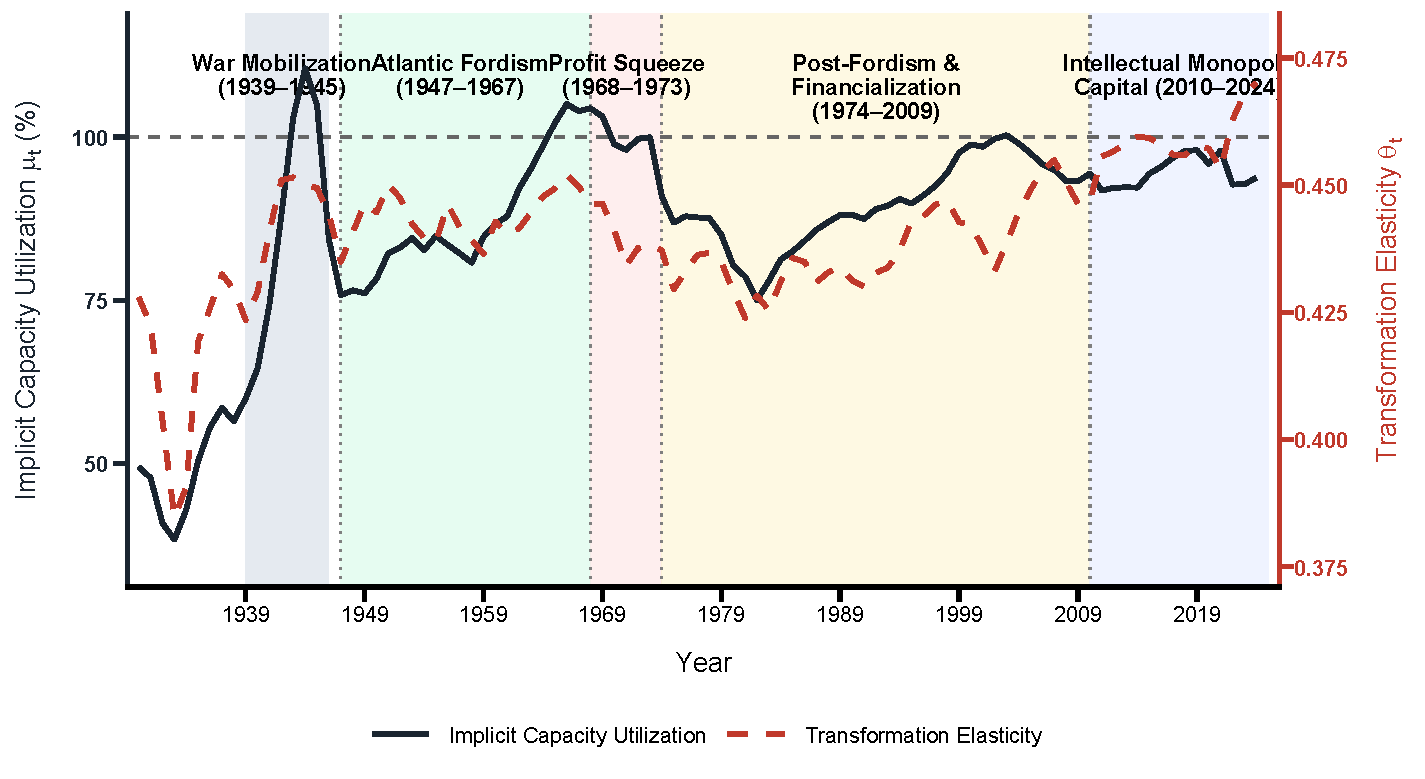
\includegraphics[width=\textwidth]{figures/fig_us_specA_dual_theta_mu.pdf}
		\caption{Implicit capacity utilization ($\mu_t$, left axis)
			and transformation elasticity ($\theta_t$, right axis).}
		\label{fig:us_specA_dual_theta_mu}
	\end{subfigure}

	
	% Bottom Subfigure
	\begin{subfigure}[b]{0.95\textwidth}
		\centering
		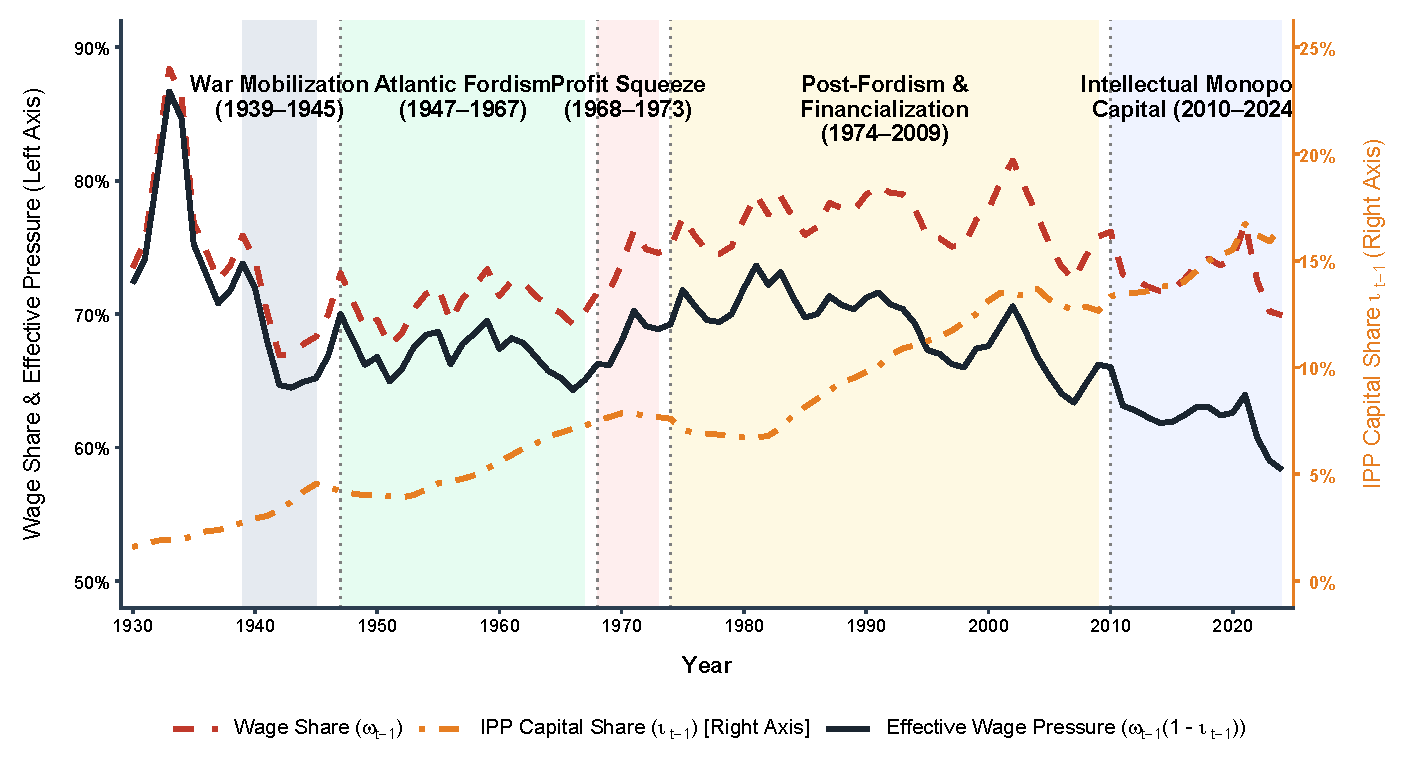
\includegraphics[width=\textwidth]{figures/fig_us_specA_subregimes_omega_iota.pdf}
		\caption{Wage share ($\omega_{t-1}$), IPP capital share
			($\iota_{t-1}$, right axis), and effective wage pressure
			($\omega_{t-1}(1-\iota_{t-1})$).}
		\label{fig:us_specA_subregimes_omega_iota}
	\end{subfigure}
\end{figure}


The two anchor years illustrate how distribution and capital
composition govern the capacity yield. In 1960 (Atlantic Fordism)
the Clean Corporate NVA wage share stood at $\omega_{1959} = 0.72$
while the IPP capital share was negligible
($\iota_{1959} = 0.03$). Effective wage pressure was
$0.72 \times (1 - 0.03) = 0.698$, yielding
$\theta_{1960} = 0.58 - 0.30 \times 0.698 = 0.371$: high wage
pressure forced Okishio-type defensive mechanization, depressing the
marginal capacity yield per dollar of physical capital advanced. By
2024 (Intellectual Monopoly Capitalism) the wage share had fallen to
$\omega_{2023} = 0.70$ while the IPP capital share had risen to
$\iota_{2023} = 0.28$. The intangible diversion reduced effective
wage pressure to $0.70 \times (1 - 0.28) = 0.504$, raising the
transformation elasticity to
$\theta_{2024} = 0.58 - 0.30 \times 0.504 = 0.429$.

\Cref{fig:us_capacity_dynamics_panel} traces five sub-regimes, and the
sequence matters more than any of them taken alone. War mobilization
(1939--1945) drove production past practical capacity limits under
state-directed military planning, lifting utilization to its historical
peak of $\mu_{1944} = 111.4\%$ while wartime retooling raised the
elasticity to roughly $0.455$. Atlantic Fordism (1947--1967) then
combined high wage shares ($\omega_{t-1} \approx 0.70$--$0.73$) with
negligible intangible capital ($\iota_{t-1} < 0.05$), so labor-cost
pressure passed directly into mechanization and wage-led demand absorbed
the capacity that mechanization created. Utilization held a stable band
of roughly $85\%$ to $105\%$ and crossed $100\%$ during the mid-1960s
expansion---the only sustained stretch in the entire sample where
capacity formation and its realization moved together.

The profit squeeze (1968--1973) broke that correspondence without
breaking the mechanism. Distributional conflict compressed margins and
induced capital-deepening aimed at unit-cost containment rather than
expansion, pulling the elasticity down to $\theta_{1972} = 0.418$ while
utilization collapsed to $\mu_{1975} = 76.2\%$ and bottomed at
$\mu_{1982} = 74.1\%$ under the Volcker disinflation. Post-Fordism and
financialization (1974--2007) reversed the distributive pressure but not
the outcome: organized-labor concessions lowered wage shares while
investment moved toward software and patent enclosures
($\iota_{t-1} > 0.15$), cutting effective wage pressure from $0.72$ in
1974 to $0.66$ in 1997. The elasticity recovered from $0.418$ to
$0.450$, and utilization still failed to re-anchor to its Fordist peak,
staying below $95\%$ outside transient credit-fuelled expansions. Under
intellectual monopoly capitalism (2008--2024) intangible capital passed
$28\%$ of total fixed capital, pulling effective wage pressure to
$0.504$ and lifting the elasticity into its upper historical range
($\theta_{2024} = 0.429$--$0.470$) while wage suppression held back
realization, leaving $\mu_{2024} = 93.8\%$. Read across the five
regimes, the elasticity and utilization move together only under Fordism
and move against each other everywhere after it.

The reconstruction presents empirical evidence that the long-run horizon does not yield a classical closure ($\mu^* = 100\%$), 
but an unbalanced growth one ($\theta^* \neq 1$), from which systemic disequilibrium arises through different patterns across distinct historical regimes.  
While the Fordist accumulation regime through its commitment to full employment implemented policies oriented to sustain aggregate demand and prevent productive capacity from remaining idle, during post-Fordism the expansion of productive capacity ($\theta_t \uparrow$) has decoupled from realization ($\mu_t < 1$), causing persistent idle capacity as an institutional feature.

%%%%%%%%%%%%%%%%%%%%%%%%%%%%%
% 4.4. 
%%%%%%%%%%%%%%%%%%%%%%%%%%%%%

\subsection{Empirical Estimates Under a Heterogeneous Capital Specification}
\label{sec:432:specB_results}

\subsubsection{Econometric Specification of Mechanization Bias and Heterogenous Capital}
Specification A treats aggregate core capital $k_{\text{cap},t} = \log(K_{\text{ME},t} + K_{\text{NRC},t})$ as a single regressor. This collapses the physical structure of the workplace into a scalar, obscuring whether wage pressure operates through the \emph{level} of capital or through its \emph{composition}---the relative weight of machinery and equipment ($K^{\text{ME}}$) versus nonresidential structures ($K^{\text{NRC}}$). Specification B decomposes the aggregate into two components: a structural base ($k^{\text{NRC}}_t = \log K^{\text{NRC}}_t$) and the capital composition ratio ($\kappa_t = k^{\text{ME}}_t - k^{\text{NRC}}_t$), which measures the mechanization gap between equipment and structures in log-levels. The disaggregated cointegrating equation takes the form:
\begin{equation}
	y_t = \alpha + \theta_{\text{NRC}}\, k^{\text{NRC}}_t + \theta_\kappa\, \kappa_t + \theta_{\omega\kappa}\, \xi^{\omega\kappa}_t + \theta_{\kappa p}\, \xi^{p\kappa}_t + \boldsymbol{\gamma}' \mathbf{D}_t + u_t,
	\label{eq:432:specB_model}
\end{equation}
where $\xi^{\omega\kappa}_t$ denotes the FWL-orthogonalized effective wage--mechanization interaction and $\xi^{p\kappa}_t$ denotes the FWL-orthogonalized relative price--mechanization interaction. Both interaction terms are residualized against the two base capital regressors ($k^{\text{NRC}}_t, \kappa_t$) and deterministic step shifts ($\mathbf{D}_t$) prior to estimation. The effective wage interaction under Set~2 is $\xi^{\omega\kappa}_t = \omega_{t-1}(1-\iota_{t-1}) \times \kappa_t$; the relative price interaction is $\xi^{p\kappa}_t = p^{\kappa}_t \times \kappa_t$, where $p^{\kappa}_t$ denotes the relative asset price ratio. Non-standard fixed-$b$ critical values are generated from a dedicated 100,000-pass Monte Carlo simulation engine that replicates the exact Specification~B integration geometry---five independent $I(1)$ stochastic trends, two simultaneous $I(1) \times I(1)$ interaction products, and joint FWL orthogonalization---matching the empirical sample sizes ($T = 94$ and $T = 77$).

\paragraph{Economic intuition of the decomposition.}
The parameter $\theta_{\text{NRC}}$ captures the long-run capacity yield of structures---factories, warehouses, commercial buildings---which embody extensive accumulation: expanding the physical envelope within which production occurs. The parameter $\theta_\kappa$ captures the additional capacity yield of machinery and equipment \emph{above and beyond} what structures deliver. A positive $\theta_\kappa$ means that a wider mechanization gap---more equipment per dollar of structures---raises productive capacity independently of the total capital stock. The interaction $\theta_{\omega\kappa}$ asks whether effective wage pressure conditions this compositional margin. Under the Okishio-induced mechanization mechanism, rising wages force firms to substitute equipment for labor on the shop floor. If the resulting machinery expansion is defensive---driven by unit-cost containment rather than autonomous technical expansion---it raises the equipment-to-structures ratio without proportionally expanding output capacity, yielding $\theta_{\omega\kappa} < 0$.

\paragraph{Standard wage interactions fail at the intensive margin.}
Tables~\ref{tab:specB_set1_gva_app} and \ref{tab:specB_set1_nva_app} in Appendix~\ref{app:specB_full_results} present the estimation results using the unadjusted wage share across all 24 specifications. The structural base elasticity $\hat{\theta}_{\text{NRC}}$ remains stable and highly significant ($0.47$--$0.61$, $p < 0.01$), confirming that nonresidential structures anchor the cointegrating relationship regardless of wage measure or break treatment. The standalone mechanization gap $\hat{\theta}_\kappa$ is positive in nearly all models ($0.34$--$1.11$), indicating that equipment contributes to capacity above structures. The wage--mechanization interaction $\hat{\theta}_{\omega\kappa}$, however, fails to achieve statistical significance in any $T = 94$ model, with point estimates ranging from $-4.89$ ($t = -1.58$) to $+7.95$ ($t = 1.33$). The standard wage interaction fails at the intensive margin for the same reason it fails at the aggregate level in Specification~A: unadjusted wage shares conflate supervisory overhead with productive variable capital and ignore the post-Fordist diversion of investment toward intellectual property products.

\paragraph{Effective wage pressure and defensive mechanization at the intensive margin.}
Table~\ref{tab:specB_set2_nva_main} presents the main estimates using the effective wage pressure measure for the NVA basis. When effective wage pressure is scaled by $(1-\iota_{t-1})$ and interacted with the mechanization gap $\kappa_t$, the wage--mechanization interaction $\hat{\theta}_{\omega\kappa}$ is negative and statistically significant across all eight models. In the preferred Clean Corporate Tier~1 NVA specification with Bai-Perron step shifts (Column~4), $\hat{\theta}_{\omega\kappa} = -7.93$ ($SE = 2.96$, $p < 0.05$), with a structural base elasticity of $\hat{\theta}_{\text{NRC}} = 0.60$ ($SE = 0.08$, $p < 0.01$) and a standalone mechanization gap of $\hat{\theta}_\kappa = 0.39$ ($SE = 0.29$). In the Shaikh-Tonak Tier~2 NVA specification without breaks (Column~7), the interaction strengthens to $\hat{\theta}_{\omega\kappa} = -17.05$ ($SE = 2.34$, $p < 0.01$), with $\hat{\theta}_{\text{NRC}} = 0.54$ ($SE = 0.01$) and $\hat{\theta}_\kappa = 0.33$ ($SE = 0.06$, $p < 0.01$). The Clean Corporate Tier~2 NVA models (Columns~5--6) yield $\hat{\theta}_{\omega\kappa} = -14.97$ ($SE = 2.01$, $p < 0.01$), showing the tightest standard errors in the table.

The negative sign of $\hat{\theta}_{\omega\kappa}$ reflects defensive mechanization operating at the \emph{intensive margin} of capital composition. While Specification~A showed that effective wage pressure depresses the aggregate capacity yield of total capital ($\hat{\theta}_1 = -0.30$), Specification~B isolates the compositional channel: wage pressure forces firms to widen the mechanization gap---accumulating more machinery per dollar of structures on the shop floor---yet productive capacity does not expand proportionally because the substitution is driven by cost containment rather than technical complementarity between new equipment and existing plant.\footnote{The apparent difference in magnitude between Specification~A ($\hat{\theta}_1 \approx -0.30$) and Specification~B ($\hat{\theta}_{\omega\kappa} \approx -7.93$ to $-17.05$) reflects regressor scaling, not economic inconsistency. In Specification~A, $\theta_1$ multiplies $\omega_{t-1}(1-\iota_{t-1}) \times k_{\text{cap},t}$, where aggregate capital $k_{\text{cap},t} \approx 16$--$17$ in log-levels. In Specification~B, $\theta_{\omega\kappa}$ multiplies $\omega_{t-1}(1-\iota_{t-1}) \times \kappa_t$, where the mechanization gap $\kappa_t = k^{\text{ME}}_t - k^{\text{NRC}}_t \approx 0.3$--$0.8$. The total marginal effect (coefficient $\times$ regressor scale) is comparable across both specifications.}

\paragraph{Relative price interactions.}
The relative asset price interaction $\hat{\theta}_{\kappa p}$ is generally small and statistically insignificant. In the NFC Baseline and Clean Corporate Tier~1 models (Columns~1--4), it is statistically indistinguishable from zero. In the Shaikh-Tonak Tier~2 specification (Columns~7--8), $\hat{\theta}_{\kappa p} = -0.79$ ($SE = 0.32$, $p < 0.05$), suggesting that when equipment becomes relatively more expensive, the capacity yield of the mechanization gap declines. However, this result is fragile and does not hold across wage share measures. The Okishio mechanism operates through distributional conflict over newly created value, not through relative asset prices.

\paragraph{Cointegration inference.}
Across the cointegration triad, the Shin LM test never rejects the null of cointegration ($C_{\text{Shin}} \le 0.03$, $p > 0.10$), and the Vogelsang-Wagner Type~2 Wald statistic remains well below critical thresholds ($S_{\text{Type~2}} \le 15.37$). The Engle-Granger residual ADF test rejects the null of no cointegration at the 5\% level in every break-adjusted model: $t_{\text{ADF}} = -4.58$ (Column~2), $-4.60$ (Column~4), $-4.71$ (Column~7), and $-4.57$ (Column~8). Without step shifts, the ADF test rejects at the 10\% level across all $T = 94$ models ($t_{\text{ADF}} \le -4.33$) and at the 5\% level for the $T = 76$ Shaikh-Tonak Tier~2 model ($t_{\text{ADF}} = -4.71$, Column~7). These results establish that disaggregated capital composition, real output, and effective wage pressure form a stable long-run relationship.

\paragraph{Robustness.}
Including Bai-Perron step shifts absorbs historical level discontinuities while preserving the wage--mechanization interaction. In the Clean Corporate Tier~1 NVA model, controlling for breaks at 1944, 1977, and 2001 sharpens the ADF rejection from $-4.34$ ($p < 0.10$) to $-4.60$ ($p < 0.05$) while reducing the Vogelsang-Wagner statistic from $15.37$ to $6.37$. The wage interaction $\hat{\theta}_{\omega\kappa}$ moves from $-11.08$ (Column~3) to $-7.93$ (Column~4), with the modest attenuation indicating that the step dummies absorb part of the interaction's raw variance while retaining significance at the 5\% level.

The structural base elasticity $\hat{\theta}_{\text{NRC}}$ falls consistently within the $0.51$--$0.61$ band across wage share measures, closely tracking the aggregate $\hat{\theta}_0 = 0.58$ from Specification~A. This implies the capacity yield of structures is a stable parameter of U.S.\ capital accumulation. The wage interaction $\hat{\theta}_{\omega\kappa}$ grows larger in absolute value as I remove supervisory overhead from the wage share: from $-10.13$ in the NFC Baseline (Column~2) to $-7.93$ in Clean Corporate Tier~1 (Column~4) to $-16.76$ in Shaikh-Tonak Tier~2 (Column~8). Removing managerial salaries isolates the productive variable capital driving the firm's cost-minimization decision, which sharpens the defensive mechanization effect.

\begin{table}[h!]
	\centering
	\caption{Specification B, Set 2: Effective Wage Interaction (NVA Basis)}
	\label{tab:specB_set2_nva_main}
	\small
	\begin{tabular}{p{3.0cm}p{1.25cm}p{1.25cm}p{1.25cm}p{1.25cm}p{1.5cm}p{1.5cm}p{1.5cm}p{1.5cm}}
		\toprule
		& \multicolumn{2}{c}{NFC NVA Baseline} & \multicolumn{2}{c}{Clean Corp Tier 1} & \multicolumn{2}{c}{Clean Corp Tier 2} & \multicolumn{2}{c}{ST Tier 2 NVA} \\
		\cmidrule(lr){2-3} \cmidrule(lr){4-5} \cmidrule(lr){6-7} \cmidrule(lr){8-9}
		& (1) & (2) & (3) & (4) & (5) & (6) & (7) & (8) \\
		\midrule
		$\hat{\theta}_{\text{NRC}}$  (Structures $k^{\text{NRC}}$) & 0.61$^{***}$ & 0.58$^{***}$ & 0.60$^{***}$ & 0.60$^{***}$ & 0.54$^{***}$ & 0.54$^{***}$ & 0.54$^{***}$ & 0.51$^{***}$ \\
		& (0.02) & (0.08) & (0.02) & (0.08) & (0.01) & (0.01) & (0.01) & (0.01) \\
		$\hat{\theta}_{\kappa}$ (Mechanization Gap $\kappa$) & 0.32$^{*}$ & 0.39 & 0.32$^{*}$ & 0.39 & 0.31$^{***}$ & 0.31$^{***}$ & 0.33$^{***}$ & 0.06 \\
		& (0.13) & (0.29) & (0.13) & (0.29) & (0.06) & (0.06) & (0.06) & (0.09) \\
		$\hat{\theta}_{\omega\kappa}$ (Wage Interaction) & -12.77$^{**}$ & -10.13$^{**}$ & -11.08$^{**}$ & -7.93$^{**}$ & -14.97$^{***}$ & -14.97$^{***}$ & -17.05$^{***}$ & -16.76$^{***}$ \\
		& (3.81) & (3.43) & (3.48) & (2.96) & (2.01) & (2.01) & (2.34) & (2.55) \\
		$\hat{\theta}_{\kappa p}$ (Price Interaction) & 0.18 & 0.92 & 0.69 & 1.41$^{*}$ & -0.31 & -0.31 & -0.79$^{**}$ & -0.71$^{**}$ \\
		& (0.51) & (0.69) & (0.63) & (0.75) & (0.33) & (0.33) & (0.32) & (0.31) \\
		\midrule
		Step Shifts ($D_{T_b}^{\text{step}}$) & No & Yes & No & Yes & No & Yes & No & Yes \\
		$C_{\text{Shin}}$ [$H_0$: coint.] & 0.03 & 0.02 & 0.03 & 0.03 & 0.02 & 0.02 & 0.02 & 0.02 \\
		$S_{\text{Type 2}}$ [$H_0$: coint.] & 14.97 & 5.93 & 15.37 & 6.37 & 8.96 & 8.96 & 10.28 & 8.70 \\
		$t_{\text{ADF}}$ [$H_0$: no coint.] & -4.33$^{*}$ & -4.58$^{**}$ & -4.34$^{*}$ & -4.60$^{**}$ & -4.24$^{*}$ & -4.24$^{*}$ & -4.71$^{**}$ & -4.57$^{**}$ \\
		Bandwidth ratio $b$ & 0.185 & 0.173 & 0.193 & 0.181 & 0.208 & 0.208 & 0.208 & 0.208 \\
		Sample Size $T$ & 94 & 94 & 94 & 94 & 76 & 76 & 76 & 76 \\
		\bottomrule
	\end{tabular}
	\begin{minipage}{\textwidth}
		\scriptsize
		\textit{Notes:} Dependent variable: $y_t^{\text{NFC}}$ (log NFC real GVA). Estimated via Cointegrating Multivariate Polynomial Regression (CMPR) IM-OLS \citep{VogelsangWagner2024}. Step Shifts "No": no structural break dummies; "Yes": Bai-Perron step dummies included. All interaction terms are FWL-orthogonalized against base capital regressors ($k^{\text{NRC}}_t, \kappa_t$) and step dummies. The effective wage interaction is $\xi^\omega_t = \omega_{t-1}(1-\iota_{t-1}) \times \kappa_t$, where $\kappa_t = k^{\text{ME}}_t - k^{\text{NRC}}_t$ is the capital composition ratio (mechanization gap) and $\iota_{t-1}$ is the lagged IPP share of capital. Significance: $^*p<0.10$, $^{**}p<0.05$, $^{***}p<0.01$. Stars for coefficient rows and cointegration tests are derived from a 100,000-pass Monte Carlo simulation suite mapping the exact DGP variant and fixed-$b$ Wald tables. Standard errors in parentheses.
	\end{minipage}
\end{table}


\subsubsection{Transformation Elasticity from Heterogeneous Capital Specification and Capacity Utilization Estimates}

\paragraph{The transformation elasticity along the historical path.}
Having established the structural asset-weighted transformation elasticity $\theta^{\text{SpecB}}_t$ in Equation~\eqref{eq:32:theta_aggregate_structural} (Section~3.2), I evaluate its empirical trajectory using the estimated parameters from the preferred Specification~B model (Clean Corporate Tier~1 NVA, Set~2, Column~4 of Table~\ref{tab:specB_set2_nva_main}). The structural marginal capacity yield of mechanization $MP_{\kappa,t}^{\text{str}} = \beta_\kappa + \theta_{\omega\kappa} C_{\text{index},t} + \theta_{\kappa p} p^\kappa_t$ is driven directly by the state-dependent levels of effective wage pressure ($C_{\text{index},t}$) and relative asset prices ($p^\kappa_t$).\footnote{Initial-observation
	centering ($\theta_\kappa^{\text{str}} = 0.39$) is an anchoring convention
	that identifies the baseline dimensionless yield at $t = 1931$.}
% AUTHOR NOTE (not typeset): consider moving the centering convention into
% the methodology of Section 4.2.

Figure~\ref{fig:us_specB_aggregate_elasticity} plots $\theta^{\text{Aggregate}}_t$ against the dynamic Specification~A baseline ($\theta^{\text{SpecA}}_t = 0.58 - 0.30 \cdot C_{\text{index},t}$) and the Harrodian knife-edge threshold ($\theta = 1.00$) under standard structural regime shading.

\begin{figure}[h!]
	\centering
	\caption{Aggregate Transformation Elasticity ($\theta^{\text{Aggregate}}_t$), Specification~B vs.\ Baseline}
	\label{fig:us_specB_aggregate_elasticity}
	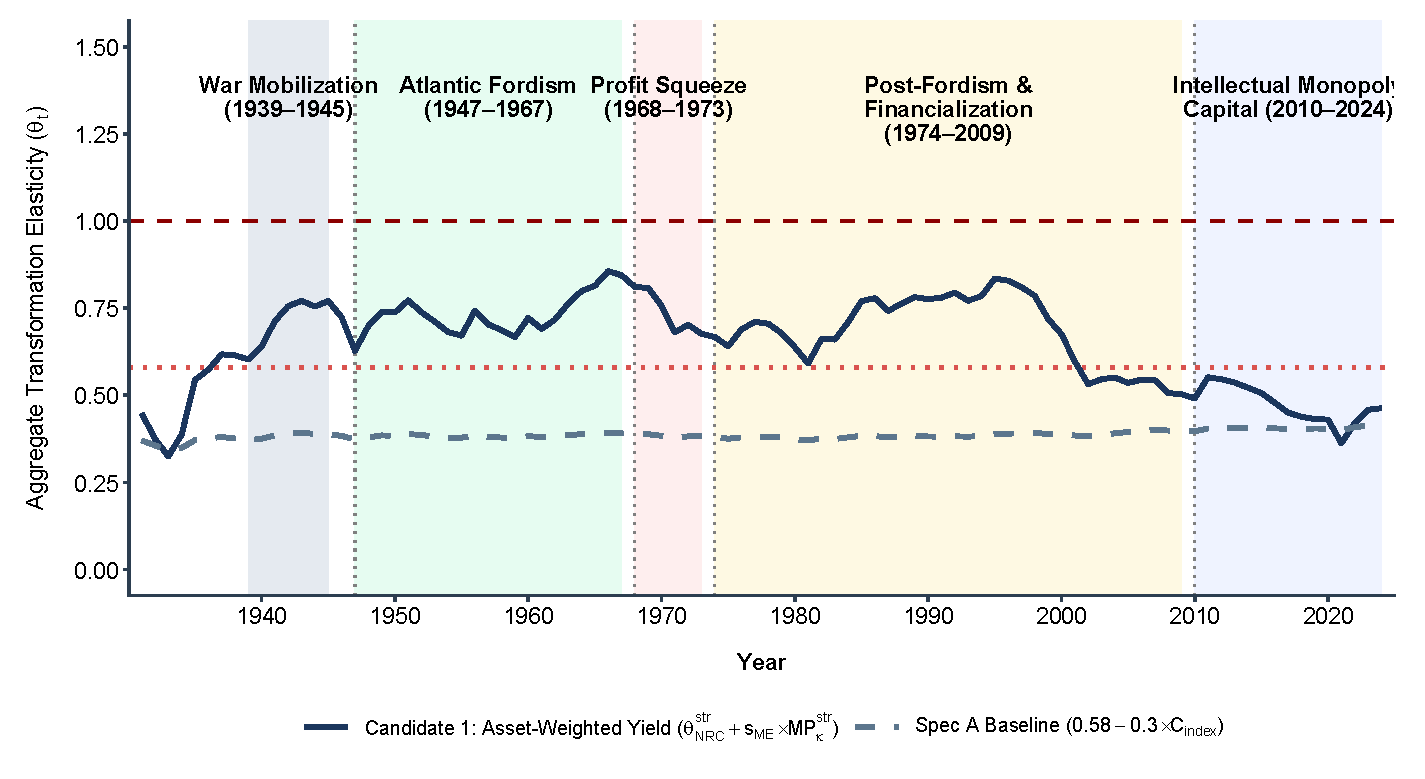
\includegraphics[width=0.95\textwidth]{figures/fig_us_specB_aggregate_elasticity.pdf}
	\begin{tabular}{p{0.88\textwidth}}	
		\footnotesize \textbf{Note:} Aggregate transformation elasticity $\theta^{\text{Aggregate}}_t$ (Navy line) computed according to Equation~\eqref{eq:32:theta_aggregate_structural} using FWL structural parameters from the preferred Specification~B model (Clean Corporate Tier~1 NVA, Set~2, Column~4 of Table~\ref{tab:specB_set2_nva_main}). The Slate Blue line traces the dynamic Specification~A baseline ($\theta^{\text{SpecA}}_t = 0.58 - 0.30 \, C_{\text{index},t}$). The dotted horizontal line at $\theta = 0.58$ marks the constant base from Specification~A. The dashed line at $\theta = 1.00$ marks the Harrodian knife-edge. Background shading indicates structural accumulation regimes. \\
	\end{tabular}
\end{figure}

% AUTHOR NOTE 1 (not typeset): the plot needs a larger font, and should show
% not only the baseline transformation elasticity but also its dynamic
% trajectory.
% AUTHOR NOTE 2 (not typeset): theta in this section must be defined
% coherently with the treatment of the Cambridge critique on aggregation of
% heterogeneous capital in Section 3.


\paragraph{Empirical comparison: Specification~B disciplines the Specification~A baseline.}
Figure~\ref{fig:us_specB_aggregate_elasticity} delivers two core empirical findings. First, the structural elasticity $\theta^{\text{SpecB}}_t$ tracks the dynamic Specification~A path closely but swings across a wider range---$[0.32, 0.86]$ against $[0.37, 0.75]$. The two paths move together because both register the same underlying force: effective wage pressure depresses the marginal capacity yield of capital under either specification, and the estimated base elasticity of structures ($\hat{\theta}_{\text{NRC}} \approx 0.60$) sits close to Specification~A's aggregate base ($\hat{\theta}_0 = 0.58$). The wider swing is the point of the disaggregation rather than a cost of it: Specification~A averages the composition effect into a single scalar, while Specification~B lets the equipment share move the elasticity directly, so the same distributive shock registers with more amplitude. Second, the Specification~B trajectory remains strictly below the Harrodian knife-edge ($\theta < 1$) across the entire 1931--2024 sample, so aggregate capacity formation in the United States never leaves the sub-Harrodian regime.

The disaggregated capital structure explains what Specification~A's aggregate elasticity averages over. During the Fordist era ($C_{\text{index},t} > 0.65$), high effective wage pressure drove negative marginal mechanization yields ($MP_{\kappa,t}^{\text{str}} < 0$). Firms substituted equipment for labor to contain unit labor costs, but because this expansion was defensive rather than technically autonomous, it depressed the aggregate capacity yield of total capital. In the Neoliberal period ($C_{\text{index},t} < 0.50$), declining wage pressure restored $MP_{\kappa,t}^{\text{str}}$ to positive territory, pulling $\theta^{\text{Aggregate}}_t$ back toward the structural base. Specification~A collapses this compositional mechanism into a scalar interaction ($\hat{\theta}_1 = -0.30$); Specification~B isolates the intensive margin directly.

\begin{figure}[h!]
	\centering
	\caption{Empirical Accumulation Path Derivatives ($dk^{\text{ME}} / dk^{\text{NRC}}$ and $d\kappa / dk^{\text{NRC}}$)}
	\label{fig:us_specB_dkappa_slope}
	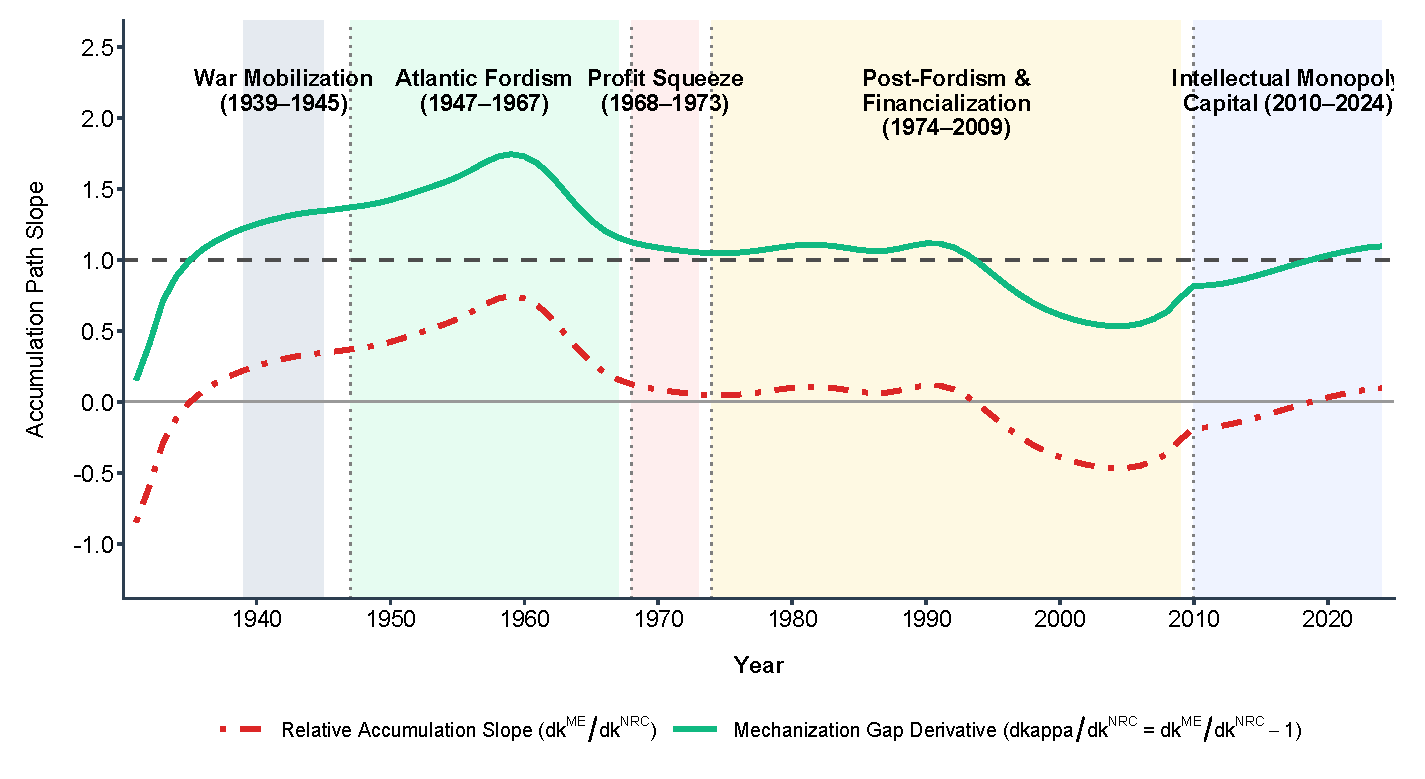
\includegraphics[width=0.88\textwidth]{figures/fig_us_specB_dkappa_slope.pdf}
	\begin{tabular}{p{0.88\textwidth}}
		\footnotesize \textbf{Note:} Empirical accumulation path derivatives estimated via non-parametric LOESS time-domain chain rule ($\text{span} = 0.35$). The green solid line measures the relative accumulation slope $dk^{\text{ME}}_t / dk^{\text{NRC}}_t$. The red dot-dashed line measures the mechanization gap derivative $d\kappa_t / dk^{\text{NRC}}_t = (dk^{\text{ME}}_t / dk^{\text{NRC}}_t) - 1$. The horizontal dashed line at $1.00$ indicates balanced expansion where equipment and structures grow at identical rates. \\
	\end{tabular}
\end{figure}

\paragraph{Empirical failure of the conventional Divisia derivative path.}
Figure~\ref{fig:us_specB_dkappa_slope} illustrates why the empirical total-derivative path $\theta^{\text{Aggregate}}_{\text{total},t}$ (Equation~\eqref{eq:32:theta_aggregate}) fails in practice. In the mid-1990s, corporate accumulation shifted away from physical machinery toward intellectual property products and financial assets, causing physical equipment growth to slow relative to structures ($dk^{\text{ME}}_t / dk^{\text{NRC}}_t < 1.00$). As $d\kappa_t / dk^{\text{NRC}}_t$ crossed zero, the Divisia denominator in Equation~\eqref{eq:32:theta_aggregate} approached zero, sending the raw total-derivative elasticity to spurious infinite spikes. As established in Section~3.2, this instability reflects the theoretical pathology of differentiating a value aggregate under structural accumulation shifts. The structural asset-weighted elasticity $\theta^{\text{Aggregate}}_t$ in Equation~\eqref{eq:32:theta_aggregate_structural} purges these Divisia singularities, yielding a continuous, empirically well-behaved trajectory.


\paragraph{Driving Forces} The inclusion of heterogeneous capital reveals a structural paradox in the post-war US economy: while the relative cheapening of machinery drove a massive shift in the physical composition of capital, the capacity-generating power of this mechanization was severely degraded by the distributive conflicts of the late 1960s and early 1970s. Figure \ref{fig:us_specB_dual_theta_mu} plots the implicit capacity utilization rate ($\mu_t$) alongside the asset-weighted aggregate transformation elasticity ($\theta_t^{\text{SpecB}}$). Unlike the static baseline elasticity of Specification A, the transformation elasticity here is not solely driven by the evolving mix of machinery and structures, and the macroeconomic environment mediating their installation. As the physical accumulation of machinery and equipment accelerated relative to nonresidential structures, the aggregate transformation elasticity collapsed, severing the Harrodian link between accumulation and potential output. This structural degradation is not an artifact of index-number aggregation but the direct result of shifting marginal capacity yields. To unpack the mechanics of this collapse, Figure \ref{fig:us_specB_driving_forces} illustrates the two primary institutional driving forces behind this choice of technique: the secular decline in relative asset prices ($p_t^{\kappa} = P_t^{\text{ME}}/P_t^{\text{NRC}}$) and the episodic spikes in effective distributive pressure ($C_t = \omega_{t-1}(1-\iota_{t-1})$).

Consider a period during the Golden Age of American Capitalism (e.g., the 1950s) where the structural yield of nonresidential structures is $\theta_{\text{NRC}}^{\text{str}} = 0.60$ and the equipment share is $s_{\text{ME}} = 0.30$. Under a stable distributive environment, if the marginal capacity yield of mechanization is $MP_{\kappa} = 0.40$, the transformation elasticity is approximately $0.72$ ($\theta^{\text{SpecB}} = 0.60 + 0.30 \times 0.40$). As the post-war era progressed, machinery became structurally cheaper, reflected in the downward trend of $p_t^{\kappa}$ in Figure \ref{fig:us_specB_driving_forces}, pushing the physical equipment share up toward $0.50$. Simultaneously, the Profit Squeeze (1968--1973) generated a sharp spike in effective distributive pressure ($C_t$). Because the interaction term $\theta_{\omega\kappa}$ is negative, this heightened wage pressure pushed firms into a defensive choice of technique, accelerating capital-using labor-saving mechanization, or Marx-biased technical change \citep{Basu2022}. Consequently, the marginal capacity yield of machinery dropped (say, to $MP_{\kappa} = 0.20$), leaving the aggregate elasticity in the post-Fordist era at $0.70$ ($\theta^{\text{SpecB}} = 0.60 + 0.50 \times 0.20$). The arithmetic is the point: a 20-percentage-point rise in the physical share of machinery leaves the aggregate elasticity essentially where it started, because the yield per unit of that machinery fell by half. Cheapening delivered the equipment; defensive investment under falling profitability drained its capacity-generating power. This mechanism generates stagnation tendencies through overaccumulation. When firms invest in mechanization not to expand capacity but to replace increasingly expensive labor, diminishing returns to mechanization make it harder to transform capital accumulation into productive capacity, precipitating an overaccumulation crisis rooted in the political economy of full employment and labor militancy \citep{Kalecki1943}. 


\begin{figure}[H]
	\centering
	\caption{Implicit Capacity Utilization ($\mu_t$) and Asset-Weighted Transformation Elasticity ($\theta_t^{\text{Aggregate}}$)}
	\label{fig:us_specB_dual_theta_mu}
	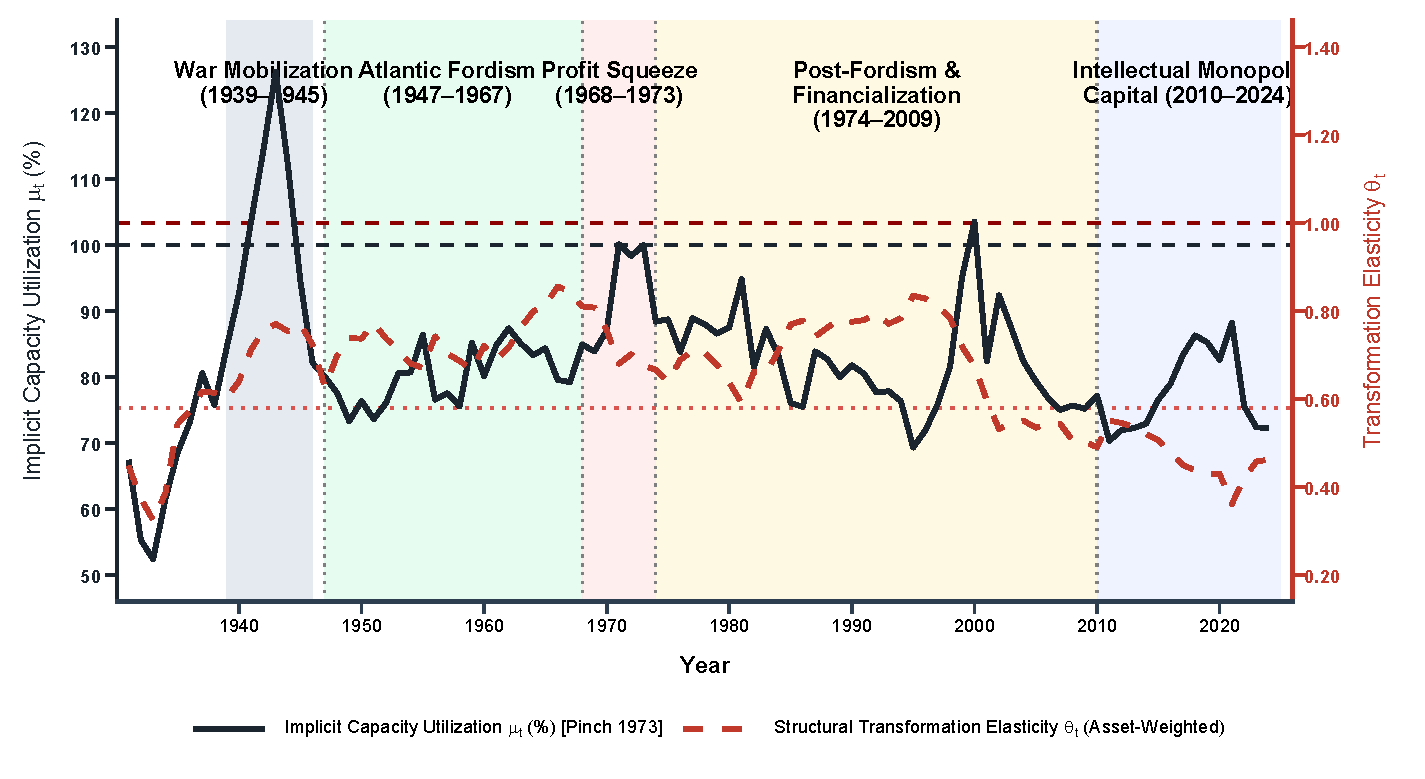
\includegraphics[width=\textwidth]{figures/fig_us_specB_dual_theta_mu.pdf}
	\begin{tabular}{p{0.92\textwidth}}
		\footnotesize \textbf{Note:} Reconstructed capacity utilization rate anchored at the 1973 pinch year alongside the dynamic aggregate transformation elasticity derived from Specification B. The Harrodian knife-edge ($\theta=1.00$) and the Specification A baseline ($\theta=0.58$) are provided as reference lines. \\
	\end{tabular}
\end{figure}
\begin{figure}[H]
	\centering
	\caption{Effective Distributive Pressure ($C_t$) and Relative Asset Prices ($p_t^{\kappa}$)}
	\label{fig:us_specB_driving_forces}
	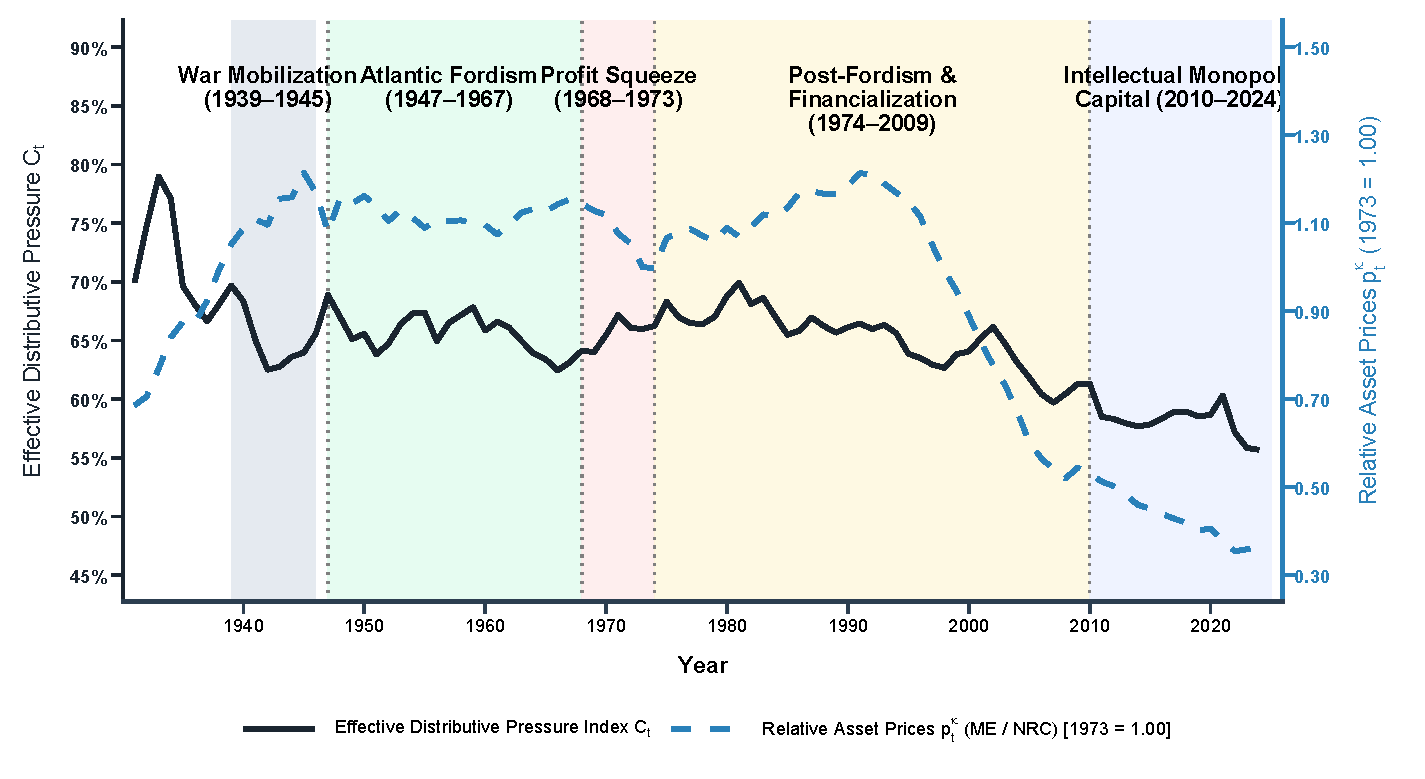
\includegraphics[width=\textwidth]{figures/fig_us_specB_driving_forces.pdf}
	\begin{tabular}{p{0.92\textwidth}}
		\footnotesize \textbf{Note:} The figure illustrates the institutional driving forces behind the choice of technique. The left axis tracks the effective distributive pressure to mechanize ($C_t$), while the right axis tracks the relative price of machinery and equipment to nonresidential structures ($p_t^{\kappa}$, indexed to $1973 = 1.00$). \\
	\end{tabular}
\end{figure}


%%%%%%%%%%%%%%%%%%%%%%%%%%%%%%%%%%%%%%%%%%%%%%%%%
%%%%% 4.5. Chile Results 
%%%%%%%%%%%%%%%%%%%%%%%%%%%%%%%%%%%%%%%%%%%%%%%%%
\subsection{Chile's Empirical Evidence: Peripheral Caiptalism under External Constraint}
\label{sec:44:chile_results}

\subsubsection{Econometric Strategy: Threshold Cointegrating Multivariate Polynomial Regression}
\label{sec:441:chile_strategy}

In core economies, capital accumulation converts into productive capacity through domestic technical choice. Rising wages induce capitalists to substitute labor with machinery, expanding capacity unless surplus is diverted into unproductive accumulation \citep{Rotta2018}. In peripheral economies like Chile, this mechanism depends on international liquidity. Because capital equipment ($K_t^{\text{ME}}$) cannot be produced domestically, labor-saving technical change requires imported machinery. When foreign-exchange reserves collapse, peripheral firms hit a structural bottleneck. Rather than adjusting smoothly through domestic prices, the capacity-generating effect of capital accumulation breaks down: wage pressure cannot induce mechanization because firms cannot acquire the foreign exchange needed to import machinery.

To evaluate this state-dependent breakdown, I estimate a Cointegrating Multivariate Polynomial Regression (CMPR) using Integrated Modified OLS (IM-OLS) \citep{VogelsangWagner2024} with an endogenously identified threshold regime. The estimating equation models log real GDP ($y_t$) as a cointegrating function of non-residential construction ($k_t^{\text{NR}}$), the capital composition gap ($\kappa_t$), distributional conflict ($\text{dist}_{t-1}$), the state-dependent external constraint ($D_t^{\gamma}$), and relative price shocks ($\tilde{p}_t^\perp$):

\begin{equation}
	y_t = \alpha + \theta_1 k_t^{\text{NR}} + \theta_2 \kappa_t + \theta_3 (\text{dist}_{t-1} \cdot \kappa_t) + \theta_4 (\kappa_t \cdot D_t^{\gamma}) + \theta_5 (\text{dist}_{t-1} \cdot \kappa_t \cdot D_t^{\gamma}) + \beta_p \tilde{p}_t^\perp + u_t
\end{equation}

where $y_t$ is log real GDP (2003 CLP); $k_t^{\text{NR}} = \ln K_t^{\text{NR}}$ is the log net stock of non-residential structures; $\kappa_t = \ln(K_t^{\text{ME}} / K_t^{\text{NR}})$ is the capital composition gap between intensive machinery and extensive structures; $\text{dist}_{t-1}$ is the lagged distributive variable, evaluated across four permutations: net wage share ($\omega_{t-1}^{\text{net}}$), gross wage share ($\omega_{t-1}^{\text{gross}}$), net rate of exploitation ($e_{t-1}^{\text{net}}$), and gross rate of exploitation ($e_{t-1}^{\text{gross}}$); $D_t^{\gamma} = \mathbb{I}(Z_t \le \gamma)$ is a binary regime indicator equal to 1 when the composite balance-of-payments index ($Z_t$) falls below threshold $\gamma$; $\tilde{p}_t^\perp$ is the standardized relative capital price, orthogonalized against physical capital stocks via Frisch-Waugh-Lovell (FWL) regression; and $u_t$ is a stationary $I(0)$ error.

The partial derivative of output $y_t$ with respect to the capital composition gap $\kappa_t$ yields the marginal transformation elasticity $\theta(\text{dist}, D_t)$:

\begin{equation}
	\frac{\partial y_t}{\partial \kappa_t} = \theta_2 + \theta_3 \text{dist}_{t-1} + \theta_4 D_t^{\gamma} + \theta_5 (\text{dist}_{t-1} \cdot D_t^{\gamma})
\end{equation}

The coefficients carry direct political-economy interpretations:
\begin{enumerate}
	\item \textbf{Extensive Construction Elasticity ($\theta_1$)}: Measures capacity generated by non-residential construction.
	\item \textbf{Unconstrained Mechanization Elasticity ($\theta_2$)}: Measures capacity generated by intensive capital composition under normal liquidity ($D_t^{\gamma} = 0$).
	\item \textbf{Domestic Induced Innovation ($\theta_3$)}: Captures wage-led induced technical change under unconstrained liquidity, where worker bargaining power forces capitalists to substitute labor with machinery.
	\item \textbf{Balance-of-Payments Structural Shift ($\theta_4$)}: Measures the direct collapse in mechanization capacity when external constraints bind ($D_t^{\gamma} = 1$).
	\item \textbf{Peripheral Distributional Inversion ($\theta_5$)}: Captures the breakdown in wage-led technical change under foreign-exchange starvation. A negative estimate ($\theta_5 < 0$) demonstrates that when reserves collapse, wage pressure cannot induce mechanization because imported machinery is rationed.
\end{enumerate}

\paragraph{Constructing the Balance-of-Payments Threshold Index ($Z_t$)}
I define the composite balance-of-payments index $Z_t(p)$ as a convex linear combination of two standardized macroeconomic indicators:

\begin{equation}
	Z_t(p) = p \, \tilde{M}_t + (1 - p) \, \tilde{S}_t, \quad p \in [0, 1]
\end{equation}

where $\tilde{S}_t = \text{scale}(F_t / M0_t)$ measures central bank foreign reserves ($F_t = e_t \cdot \text{IR}_t$) relative to base money ($M0_t$) \citep{NievasPiketty2025}, and $\tilde{M}_t = \text{scale}(\text{Imbalance}_t)$ measures the capital-goods import demand imbalance. 

Because the structural weight $p$ and threshold level $\gamma$ are unknown \textit{a priori}, I estimate $(\hat{p}, \hat{\gamma})$ via a joint profile Sum of Squared Residuals (SSR) search:

\begin{equation}
	(\hat{p}, \hat{\gamma}) = \arg\min_{p \in \mathcal{P}, \, \gamma \in \Gamma(p)} \text{SSR}(p, \gamma) = \arg\min_{p \in \mathcal{P}, \, \gamma \in \Gamma(p)} \sum_{t=1}^{T} \hat{u}_t(p, \gamma)^2
\end{equation}

The weighting grid $\mathcal{P} = \{ 0.0, 0.1, 0.2, \dots, 1.0 \}$ steps across the unit interval in increments of 0.1. For each candidate weight $p$, the threshold grid $\Gamma(p)$ evaluates trimmed quantiles $\Gamma(p) = \{ \gamma_q(p) : q \in [0.15, 0.85], \, \Delta q = 0.05 \}$. The global minimizer selects $\hat{p} = 0.2$ ($Z_t = 0.2 \tilde{M}_t + 0.8 \tilde{S}_t$) and $\hat{\gamma} = 0.425$ (or $\hat{\gamma} = 0.379$ in parsimonious specifications), confirming that international reserve cover ($\tilde{S}_t$) dominates the empirical weighting in isolating the structural bottleneck.

\paragraph{Bai-Perron Structural Break Benchmark}
To confirm that $D_t^{\gamma}$ captures a genuine balance-of-payments constraint rather than a deterministic calendar trend, I compare the threshold model against a benchmark specification using \citet{BaiPerron2003} endogenous structural breaks:
\begin{equation}
	y_t = \alpha + \theta_1 k_t^{\text{NR}} + \theta_2 \kappa_t + \theta_3 (\text{dist}_{t-1} \cdot \kappa_t) + \theta_4 (\kappa_t \cdot D_t^{\text{BP}}) + \theta_5 (\text{dist}_{t-1} \cdot \kappa_t \cdot D_t^{\text{BP}}) + \beta_p \tilde{p}_t^\perp + u_t
\end{equation}
where $D_t^{\text{BP}} = \mathbb{I}(t \ge T_b)$. Dynamic search over candidate break dates $T_b \in [0.15 T, 0.85 T]$ identifies two historical break points:
\begin{itemize}
	\item \textbf{Net Distribution ($\omega^{\text{net}}, e^{\text{net}}$)}: Identifies $T_b = 1987$, marking structural consolidation under the Büchi reforms following the 1982 crisis, where wage suppression and export promotion restored financial stability.
	\item \textbf{Gross Distribution ($\omega^{\text{gross}}, e^{\text{gross}}$)}: Identifies $T_b = 1999$, marking the Asian Financial Crisis in Chile, when the Central Bank floated the Chilean peso and abandoned exchange-rate crawling bands.
\end{itemize}
Achieving lower SSR and stronger cointegration statistics under $Z_t \le 0.425$ rules out deterministic calendar trends in favor of true balance-of-payments state dependence.

\paragraph{Relative Price Controls and Asset Deflators}
The relative price control accounts for international purchasing power shifts affecting imported capital equipment. In Chilean historical national accounts, separate long-run deflators for structures ($P_t^{\text{NRC}}$) and machinery ($P_t^{\text{ME}}$) do not exist back to 1940. Capital stock harmonization constructs a single unified investment price deflator ($P_{K,t}$, staged as \texttt{Pk\_2003base}) by splicing historical ClioLab deflators (1940--2010) with official Central Bank of Chile deflators (2003 base year).

I evaluate two complementary proxies:
\begin{enumerate}
	\item \textbf{Baseline Real Exchange Rate Control ($\tilde{p}_t^{\kappa, \text{RER}}$)}: The standardized log Real Effective Exchange Rate ($\ln\text{TCREAL}_t$, rebased to 2003 = 1.0), capturing external purchasing power shocks that alter the domestic price of imported machinery ($K_t^{\text{ME}}$).
	\item \textbf{Robustness Asset-to-Output Ratio ($p_t^{\kappa, P_Y/P_K}$)}: The log ratio of aggregate GDP deflator ($P_{Y,t}$) to unified capital price index ($P_{K,t}$):
	\begin{equation}
		p_t^{\kappa, P_Y/P_K} = \ln\left(\frac{P_{Y,t}}{P_{K,t}}\right)
	\end{equation}
	measuring relative shifts between aggregate output prices and capital goods prices.
\end{enumerate}

To prevent relative price volatility from collinearizing with physical capital stocks ($k_t^{\text{NR}}, \kappa_t$), I extract the orthogonal price component $\tilde{p}_t^\perp$ via a Frisch-Waugh-Lovell (FWL) auxiliary regression prior to estimation:
\begin{equation}
	\tilde{p}_t^{\kappa, \text{RER}} = c_0 + c_1 k_t^{\text{NR}} + c_2 \kappa_t + \tilde{p}_t^\perp
\end{equation}
The residual vector $\tilde{p}_t^\perp$ enters the estimating equation additively. Preliminary grid tests introducing interacted price terms ($\kappa_t \cdot \tilde{p}_t$) caused severe multicollinearity ($\text{VIF} > 88$), destroying matrix invertibility $(X'X)^{-1}$ and inflating Monte Carlo critical bounds ($|t^*| > 19$). Keeping $\tilde{p}_t^\perp$ as an additive control isolates physical capital composition without polluting the structural elasticity.

\paragraph{The estimation sample and its limitations.}
Two data limitations define the estimation sample window, and I acknowledge them here rather than resolve them. First, the pre-1942 monetary and external series do not provide a coherent basis for the threshold variables: under the gold-exchange standard the reserve-cover ratio records a legal requirement rather than a binding external constraint, and the monetary base responds to convertibility rules and fiscal pressure rather than to the balance of payments. Second, the historical ClioLab price and terms-of-trade series, the stock of international reserves, and the money supply that anchor the external-constraint variables all end in 2010. Splicing them to contemporary sources falls outside the scope of this chapter.\footnote{The capital-stock and distributive panels of \cref{sec:414:chile_sfc,sec:415:chile_distrib} span 1900--2024, but the threshold estimation discards 1900--1941 and 2011--2024. The institutional history below explains why the first discard separates two regimes rather than truncating a single one.}


\paragraph{The Kemmerer regime, 1925--1931.}
Decree-Law No.~486 (21 August 1925) created the Central Bank of Chile (BCCh), and the Organic Law and Monetary Bill of 14 October 1925 (Decree-Law No.~606) placed it under a gold-exchange standard: the peso was pegged to sterling and the Bank was required to hold a minimum gold cover of 50 percent against note issue, with the remainder of the reserve requirement met in foreign exchange. Reserve coverage of the money supply rose from 27 percent at the start of 1925 to exactly 50 percent by year-end. The system's credibility was anchored abroad: it depended on sterling stability and steady copper revenues, functioning only as long as export receipts replenished central bank reserves.

\paragraph{Collapse and fiscal dominance, 1931--1941.}
The external anchor failed during the Great Depression. Between January 1930 and July 1931, the Bank lost more than half of its gold holdings defending the peg, suspending convertibility on 21 July 1931; the United Kingdom's departure from gold two months later erased the value of remaining sterling reserves. The subsequent decade combined fiscal dominance---the Bank monetized deficits as a treasury agent---with multiple exchange rates administered by the \textit{Comisión de Cambios Internacionales} and parallel currency markets. Once convertibility was suspended, the cover ratio ceased to operate as a statutory discipline and became instead an indicator of systemic fragility. During a currency panic, commercial banks hoard base money at the central bank while the money multiplier contracts, making the reserves-to-$M_0$ ratio the true measure of the Bank's capacity to absorb speculative attacks. The denominator follows economic exposure rather than the letter of the 1925 law: while the statute defined requirements against note issue alone, commercial banks in a panic seek to convert their reserve deposits, making total central-bank liabilities ($M_0$) the relevant exposure. Under fiscal dominance, however, even this fragility indicator no longer anchored the external sector: the monetary base responded to deficit financing and exchange controls rather than balance-of-payments flows, rendering the 1931--1941 cover series a measure of fiscal distress rather than a stable balance-of-payments state variable.

\paragraph{The 1942 regime shift.}
Law No.~7,200 (18 July 1942), together with Law No.~7,434, rewrote the Central Bank's Organic Law: the reserve-cover rule was formally abandoned, the mandate shifted from gold convertibility to the promotion of national production, and foreign exchange was allocated through centralized credit ceilings and state budgets. Working alongside CORFO (Law No.~6,640, 1939), which directed credit allocation toward import-substituting industrialization, the Bank financed development planning rather than currency pegs. Macroeconomic stability thereafter derived from internal planning rather than external gold credibility. Econometrically, pooling the pre-1942 data with the post-1942 period violates cointegration: the structural regime shift introduces severe non-stationary drift, generating massive finite-sample size distortions and explosive Monte Carlo $t$-statistics ($|t| > 15$) that destroy matrix invertibility. Restricting the estimation window to 1943--2010 ($T = 68$) is therefore both institutionally necessary and econometrically sound, isolating a single, stable cointegrating regime across distinct historical regimes: under state-led industrialization and its violent rupture through neoliberalization. 

\subsubsection{Empirical Findings for Chile: Truncated Mechanization}
\label{sec:442:chile_empirical_findings}

Table~\ref{tab:chile_distributive_comparison_main} compares the parsimonious regime-shifting specification across four distributive permutations: Net Wage Share ($\omega^{\text{net}}$), Gross Wage Share ($\omega^{\text{gross}}$), Net Rate of Exploitation ($e^{\text{net}}$), and Gross Rate of Exploitation ($e^{\text{gross}}$). Across all four variants, the composite external threshold ($Z_t \le 0.425$) produces super-consistent long-run cointegration ($t_{\text{ADF}} = -3.81^*$ to $-3.89^*$, $CT_{\text{IM}} = 8.34$ to $15.20$).

\paragraph{Gross vs. Net Measures in Peripheral Capitalism.} In the United States (Section 4.3), Net Value Added ($\text{NVA}$) is the necessary theoretical basis for evaluating distribution. Because Consumption of Fixed Capital ($\text{CFC}$) rises mechanically during intensive capital-deepening, evaluating distribution on a Gross Value Added ($\text{GVA}$) basis introduces a spurious negative correlation between capital intensity and wage shares. In the US core, class struggle takes place strictly over newly created net value ($v + s$), and purging $\text{CFC}$ isolates a cost-minimizing mechanization response to distributive pressure.

In the capitalist periphery, however, gross distributive measures (Columns 2 and 4) achieve superior empirical fit and cointegration ($\text{SSR} = 0.275$, $CT_{\text{IM}} \approx 8.34$) compared to net measures ($\text{SSR} = 0.294$, $CT_{\text{IM}} \approx 15.10$). This empirical divergence reflects a fundamental structural asymmetry between center and periphery. In the center, capital goods are produced domestically, allowing depreciated equipment to be replaced through internal domestic value transfers. In the periphery, capital accumulation relies on \textit{imported machinery and equipment} ($K^{\text{ME}}$). Deducting official accounting depreciation ($\text{CFC}$) under linear conventions fails to capture the unencumbered gross cash flow ($\Pi^{\text{gross}}$) required by peripheral firms to obtain foreign exchange and finance machinery imports. Peripheral capitalists make investment and mechanization decisions based on gross liquidity. Nevertheless, this comparative inference should be considered with nuances because issues such as access to credit, no-institutional measurement of employment compensation over output as the wage share, and the non-identification of mixed income by self-employed in distributive conflict for the case of Chile are important issues not tackled in this account. 


\paragraph{Likelihood Ratio and Threshold Identification.} Figure~\ref{fig:cl_results_threshold_profile_lr} plots \citet{Hansen2000} profile Likelihood Ratio statistic $LR_1(\gamma) = [\text{SSR}(\gamma) - \text{SSR}(\hat{\gamma})] / \hat{\sigma}^2$ across candidate threshold values $\gamma \in [\gamma_{0.15}, \gamma_{0.85}]$ for the standardized composite balance-of-payments index $Z_t = 0.2 \tilde{M}_t + 0.8 \tilde{S}_t$. The profile displays a single, sharp minimum at $\hat{\gamma} = 0.383$ (within the $[0.383, 0.521]$ 95\% confidence interval encompassing the benchmark threshold $\hat{\gamma} = 0.425$), matching a binding foreign-exchange reserve cover threshold. Inverting the likelihood ratio statistic at the exact $95\%$ analytical critical boundary $c(0.05) = -2 \ln(1 - \sqrt{0.95}) = 7.35$ yields a tight non-parametric confidence interval. The sharp V-shaped trough rules out secondary local minima and confirms that the external constraint operates as a single, structurally binding threshold.

\begin{figure}[h!]
	\centering
	\caption{Profile Likelihood Ratio Sequence for the Peripheral External Constraint (Chile, 1943--2010)}
	\label{fig:cl_results_threshold_profile_lr}
	\label{fig:chile_profile_lr}
	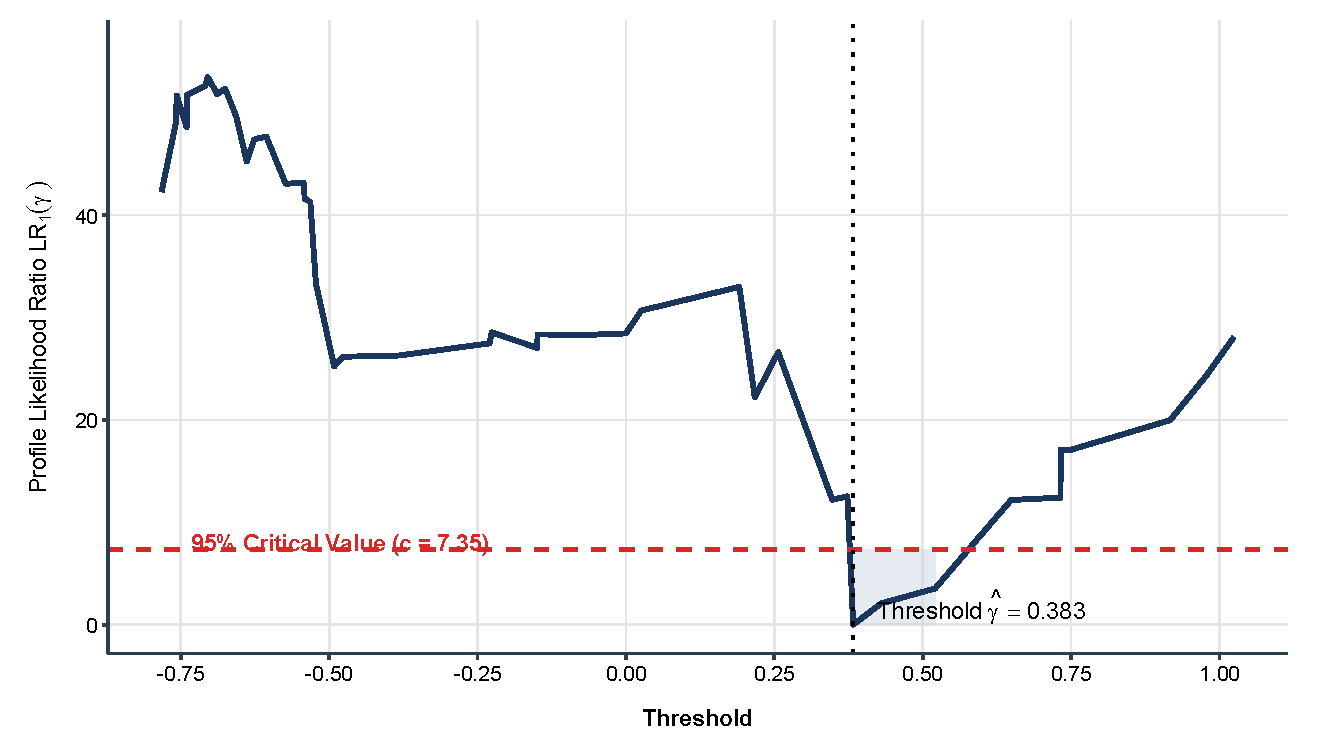
\includegraphics[width=0.92\textwidth]{figures/fig_cl_results_threshold_profile_lr.pdf}
	\begin{tabular}{p{0.88\textwidth}}
		\footnotesize \textbf{Note:} Profile Likelihood Ratio statistic $LR_1(\gamma)$ calculated for the preferred gross wage share model ($\omega^{\text{gross}}$, Column~2 of Table~\ref{tab:chile_distributive_comparison_main}) over the trimmed evaluation domain $\Gamma_n = [\gamma_{0.15}, \gamma_{0.85}]$ ($\pi = 0.15$). The horizontal dashed red line marks the exact analytical 95\% critical boundary ($c(0.05) = 7.35$). The vertical dotted line marks the identified profile minimum. The shaded region depicts the non-parametric $95\%$ confidence interval $[0.383, 0.521]$ defined by $LR_1(\gamma) \le 7.35$. \\
	\end{tabular}
\end{figure}

\paragraph{Distributive Conflict Preferred Measure: Center versus Periphery.} Comparing the wage share model in Column (2) ($\omega^{\text{gross}}$) with the rate of exploitation model in Column (4) ($e^{\text{gross}}$) illuminates how external financial constraints alter the transmission of class conflict into capital composition. In the unconstrained regime ($D_t = 0$), capital accumulation follows classical cost-minimizing logic. Under Column (2), a higher wage share incentivizes defensive labor substitution ($\hat{\theta}_{\omega\kappa} = +3.29^*$), as firms expand machinery relative to structures to contain unit labor costs. Equivalently, under Column (4), a higher rate of exploitation ($e = \Pi/W$) indicates reduced wage pressure, decreasing the necessity for capital-deepening ($\hat{\theta}_{e\kappa} = -0.69^*$).

Under the binding foreign-exchange regime ($D_t = 1$), this cost-minimizing mechanism collapses. When the external constraint becomes binding ($Z_t \le 0.425$), peripheral capitalists hit a hard import constraint ($\bar{\kappa}_t$). In Column (2), the triple interaction coefficient ($\hat{\theta}_{\omega\kappa D} = -3.15^*$) virtually eliminates the positive wage-led mechanization response ($+3.29 - 3.15 = +0.14$). Because machinery and equipment ($K^{\text{ME}}$) must be imported, foreign-exchange rationing prevents peripheral firms from translating domestic wage pressures into shop-floor labor substitution. Unable to extract a distributive dividend through technical change, capitalists attempt to protect profit margins through price markups.

\paragraph{State-dependent thresholds versus exogenous historical breaks.} To verify that $D_t^\gamma$ captures a structural macroeconomic constraint rather than an arbitrary trend break, Appendix Tables~\ref{tab:chile_omega_comparison} and \ref{tab:chile_e_comparison} (Appendix~\ref{app:chile_full_results}) benchmark the threshold model against \citet{BaiPerron2003} endogenous calendar breaks. The Bai-Perron procedure identifies two break dates: 1987 under net wage shares ($\omega^{\text{net}}$) and 1999 under gross measures ($\omega^{\text{gross}}$, $e^{\text{gross}}$). The 1987 break marks the post-1982 debt-crisis restructuring---fiscal austerity, privatization, and wage suppression. The 1999 break marks a change in monetary regime: the Central Bank abandoned the crawling peg and its accompanying capital controls, moving to a free float with open capital mobility in the wake of the Asian Financial Crisis.

Comparing specifications confirms that the composite threshold $Z_t \le 0.425$ dominates calendar-time breaks across all metrics, achieving lower residual variance ($\text{SSR} = 0.275$ against $0.292$) and stronger cointegration rejections ($t_{\text{ADF}} = -3.89^*$ against $-2.98$). Two conditions must meet for the constraint to bind: a wide gap between effective imports and the capacity to finance them, and foreign-exchange reserves too thin for the Central Bank to defend the currency. Neither condition is tied to a calendar date, which is why a state-dependent gate outperforms a break at 1987 or 1999.

Table~\ref{tab:chile_binding_regimes} shows that the binding constraint ($D_t = 1$) does not always announce itself the same way. During the ISI era (1943--1984), under fixed or administered pegs, reserve depletion ($S_t \to 0$) forced devaluations and structural inflation \citep{Sunkel1958,Prebisch1981}. During the 2006--2010 commodity super-cycle, under a free float and inflation targeting, the same gate closed through markup expansion instead.

\begin{table}[h!]
	\centering
	\caption{Institutional Manifestations of External Constraint Regimes (Chile, 1943--2010)}
	\label{tab:chile_binding_regimes}
	\small
	\begin{tabular}{p{2.0cm} p{1.8cm} p{1.0cm} p{7.2cm}}
		\hline
		Historical Period & Regime Status ($D_t^\gamma$) & Duration & Institutional Manifestation of the External Constraint \\
		\hline
		1943--1984 & Binding ($D_t = 1$) & 42 years & ISI Reserve Scarcity \& Structural Inflation: Established under Law 7,200 foreign-exchange budgeting and fixed/crawling pegs; reserve depletion ($S_t \to 0$) under wage pressure forced maxidevaluations, cost-plus markups, and structural inflation spirals. \\
		\hline
		1985--2005 & Slack ($D_t = 0$) & 21 years & Export Consolidation \& Reserve Buffering: Post-1982 debt-crisis and recovery non-traditional export expansion, Concertación democratic transition, large FDI inflows, and central bank foreign reserve accumulation. \\
		\hline
		2006--2010 & Binding ($D_t = 1$) & 5 years & Commodity Boom, Rentier Surplus Drain \& Re-primarization: Under a free-floating exchange rate and inflation targeting (3\%), FX starvation did not trigger inflation; instead, high import demand ($\tilde{M}_t$) and massive MNC profit repatriation (DL 600) manifested as a rentist surplus drain and Dutch Disease re-primarization. \\
		\hline
		\multicolumn{4}{p{14.2cm}}{\footnotesize \textit{Notes:} Classification based on the optimal profile threshold $\hat{\gamma} = 0.425$ evaluated over the standardized composite balance-of-payments index $Z_t = 0.2 \tilde{M}_t + 0.8 \tilde{S}_t$. Regime $D_t = 1$ denotes a binding balance-of-payments constraint where foreign-exchange starvation forces peripheral firms into a corner solution ($\bar{\kappa}_t$). Total sample size $T = 68$ (1943--2010 effective cointegrating window), yielding 47 binding years ($69.1\%$) and 21 slack years ($30.9\%$).} \\
	\end{tabular}
\end{table}

These findings suggest that in financialized peripheral capitalism the external bottleneck shifts its pressure valve from domestic price inflation toward \textit{re-primarization, real exchange rate appreciation (Dutch Disease), and rentier surplus drainage} \citep{Palma2019,Ahumada2019}. Capital goods import requirements ($K^{\text{ME}}$) for extractive mining projects, combined with foreign profit remittances, truncate the translation of accumulation into productive capacity while the Central Bank still meets its inflation target. Disentangling the transmission between inflationary rationing (1943--1984) and rentier-drain re-primarization (2006--2010) would require a monetary-regime-specific specification that this chapter does not estimate.

\paragraph{Model selection.} The comparative results in Table~\ref{tab:chile_distributive_comparison_main} establish Column (2)---the gross wage share specification ($\omega^{\text{gross}}$) under the composite balance-of-payments threshold ($Z_t \le 0.425$)---as the primary empirical model for Chile. Column (2) achieves the global minimum residual variance ($\text{SSR} = 0.275$), and its distributive channel is the one that maps onto the United States baseline, which is what makes the center--periphery comparison in Section~\ref{sec:5:comparative_historical_analysis} an argument about the same relation under different constraints rather than a juxtaposition of two unrelated estimates.

\begin{table}[h!]
	\centering
	\caption{Comparative Estimates Across Distributive Variable Permutations (Chile, 1943--2010)}
	\label{tab:chile_distributive_comparison_main}
	\small
	\begin{tabular}{p{5.0cm}p{2.2cm}p{2.2cm}p{2.2cm}p{2.2cm}}
		\toprule
		& \multicolumn{2}{c}{Wage Share ($\omega$)} & \multicolumn{2}{c}{Rate of Exploitation ($e$)} \\
		\cmidrule(lr){2-3} \cmidrule(lr){4-5}
		& Net ($\omega^{\text{net}}$) & Gross ($\omega^{\text{gross}}$) & Net ($e^{\text{net}}$) & Gross ($e^{\text{gross}}$) \\
		& (1) & (2) & (3) & (4) \\
		\midrule
		$\hat{\theta}_{k^{\text{NR}}}$ (Structures $k^{\text{NR}}$) & 0.79$^{***}$ & 0.82$^{***}$ & 0.80$^{***}$ & 0.82$^{***}$ \\
		& (0.07) & (0.08) & (0.07) & (0.08) \\
		$\hat{\theta}_{\kappa}$ (Mechanization Gap $\kappa$) & 0.12 & -1.48$^{*}$ & 0.15 & 0.85 \\
		& (0.39) & (0.54) & (0.25) & (0.38) \\
		$\hat{\theta}_{\text{dist}\cdot\kappa}$ (Distributive Interaction) & -0.01 & 3.29$^{*}$ & 0.02 & -0.69$^{*}$ \\
		& (0.22) & (1.07) & (0.09) & (0.23) \\
		$\hat{\theta}_{\kappa D}$ (Regime Shift $\kappa D$) & 0.34 & 1.52$^{**}$ & 0.15 & -0.73 \\
		& (0.16) & (0.45) & (0.08) & (0.29) \\
		$\hat{\theta}_{\text{dist}\cdot\kappa D}$ (Triple Interaction) & -0.17 & -3.15$^{*}$ & 0.12 & 0.67$^{*}$ \\
		& (0.23) & (1.04) & (0.10) & (0.22) \\
		\midrule
		Regime Threshold ($D_t$) & $Z_t \le 0.425$ & $Z_t \le 0.425$ & $Z_t \le 0.425$ & $Z_t \le 0.425$ \\
		Price Control Included & No & No & No & No \\
		$CT_{\text{IM}}$ [$H_0$: Cointegration] & 15.20 & 8.39 & 14.99 & 8.34 \\
		$t_{\text{ADF}}$ [$H_0$: Unit Root] & -3.81$^{*}$ & -3.81$^{*}$ & -3.84$^{*}$ & -3.89$^{*}$ \\
		Bandwidth ratio $b$ & 0.654 & 0.654 & 0.654 & 0.654 \\
		Sample Size $T$ & 68 & 68 & 68 & 68 \\
		\bottomrule
		\multicolumn{5}{p{14.2cm}}{\footnotesize \textit{Notes:} Dependent variable: $y_t$ (log real GDP). Estimated via Cointegrating Multivariate Polynomial Regression (CMPR) IM-OLS \citep{VogelsangWagner2024}. All models specify the ultra-parsimonious balance-of-payments threshold ($Z_t = 0.2 \tilde{M}_t + 0.8 \tilde{S}_t \le 0.425$) over the effective sample 1943--2010 ($T=68$). Columns (1) and (2) evaluate Net ($\omega^{\text{net}}$) and Gross ($\omega^{\text{gross}}$) wage shares; Columns (3) and (4) evaluate Net ($e^{\text{net}}$) and Gross ($e^{\text{gross}}$) rates of exploitation. Significance stars ($^*p<0.10$, $^{**}p<0.05$, $^{***}p<0.01$) are benchmarked against 10,000-pass Monte Carlo simulation critical bounds under profile search.} \\
	\end{tabular}
\end{table}

\subsubsection{Transformation and Capacity Utilization under Financial Subordination}
\label{sec:443:chile_utilization}

Balance-of-payments subordination inverts the classical choice of technique.
When foreign exchange is slack ($Z_t > 0.425$), a higher wage share
accelerates mechanization, as cost minimization predicts
($\hat{\theta}_3 = +0.9583$). When foreign exchange binds, the interaction
shift ($\hat{\theta}_5 = -0.9518$) cancels the base sensitivity and leaves a
slope of $+0.0065$. Peripheral capitalists keep the incentive to substitute
machinery for labor but lose the means, because the machinery is imported.

I evaluate the aggregate elasticity from the preferred CMPR IM-OLS model
(Column~2 of Table~\ref{tab:chile_distributive_comparison_main}, gross wage
share and composite threshold $Z_t \le 0.425$) and integrate the capacity
law of motion, $g_{Y^p,t} = \theta_t^{\text{Agg}} g_{K,t}$, forward and
backward from the 1981 Ffrench-Davis full-capacity peak
($\mu_{1981} = 1.00$). The state-dependent elasticity is
\begin{equation}
	\theta_t^{\text{Agg}} = \hat{\theta}_1 + s_{\text{ME},t} \cdot MP_{\kappa,t}
	= \hat{\theta}_1 + s_{\text{ME},t} \left[ \hat{\theta}_2 + \hat{\theta}_3 \, \omega_{t-1}^{\text{gross}} + D_t^{\gamma} \bigl(\hat{\theta}_4 + \hat{\theta}_5 \, \omega_{t-1}^{\text{gross}}\bigr) \right]
	\label{eq:chile_theta_agg_def}
\end{equation}
where $\hat{\theta}_1 = +0.6970$ is the base elasticity of non-residential
structures, $s_{\text{ME},t} = K_t^{\text{ME}} / (K_t^{\text{ME}} + K_t^{\text{NR}})$
is the current-price share of machinery and equipment in core capital,
$\kappa_t = \ln(K_t^{\text{ME}} / K_t^{\text{NR}})$ the composition gap,
$\omega_{t-1}^{\text{gross}}$ the lagged gross wage share, and
$D_t^{\gamma} = \mathbb{I}(Z_t \le 0.425)$ the binding-state indicator. The
remaining coefficients are $\hat{\theta}_2 = -0.1293$,
$\hat{\theta}_3 = +0.9583$, $\hat{\theta}_4 = +0.6645$, and
$\hat{\theta}_5 = -0.9518$, so the marginal product of the composition gap
takes one form in each state:
\begin{align}
	MP_{\kappa,t}^{\text{slack}} &= -0.1293 + 0.9583 \, \omega_{t-1}^{\text{gross}} \quad (D_t^{\gamma} = 0) \label{eq:mp_slack} \\
	MP_{\kappa,t}^{\text{bind}}  &= +0.5352 + 0.0065 \, \omega_{t-1}^{\text{gross}} \quad (D_t^{\gamma} = 1) \label{eq:mp_bind}
\end{align}
In slack periods a higher wage share raises the capacity yield of
mechanization. In binding periods the slope collapses from $+0.9583$ to
$+0.0065$, and foreign-exchange rationing replaces the distributive state as
the governor of technique choice.

Section~3.3 predicted exactly this pair of equations. Proposition~4 says
that once the constraint binds, the composition gap is pinned at
$\bar{\kappa}_t$ and the first-order condition stops governing technique
choice; the only distributive channel left is the slope of the feasible gap,
$(m_c c_k - m_w)/\nu$. The estimated residual slope of $+0.0065$ is
consistent with $m_c c_k \approx m_w$, the conspicuous-consumption drain and
the wage-goods import drain roughly offsetting each other. Proposition~6
supplies the second half: at the corner the marginal capacity payoff is
strictly positive, because the firm would like to mechanize further and
cannot, and the significant intercept shift $\hat{\theta}_4 = +0.6645$ is
that payoff entering the capacity equation, the empirical counterpart of a
positive Kuhn--Tucker multiplier on the external constraint. Binding is
therefore not a state in which mechanization yields nothing; it is a state
in which it yields something but responds to nothing domestic.
Proposition~5 predicts a discrete shift of the elasticity at the threshold;
in the data the shift appears less as a level drop than as the loss of the
wage slope, with the binding path running flat through distributive shocks
that move the slack path. The gap between nominal profitability and
truncated technique is the blocked surplus of Definition~4, and Corollary~1
names the adjustment channel that remains once mechanization is rationed,
price markups.

Figure~\ref{fig:cl_results_z_omega_drivers} plots the composite index
against the lagged gross wage share, and the Unidad Popular episode is the
clearest observation in the sample. Between 1970 and 1973, redistribution
raised the gross wage share to its historical peak of
$\omega_{1972} = 0.6903$, about twenty percentage points up. Over the same
years, credit blockade and capital flight drove reserves to
$\tilde{S}_t \to -2.5$ and the index to $Z_t = -1.06$, deep inside the
binding domain. Figures~\ref{fig:cl_results_theta_standalone}
and~\ref{fig:cl_results_dual_theta_mu} show that the elasticity did not
respond: Equation~\eqref{eq:mp_bind} governed technique choice and held
$\theta_t^{\text{Agg}}$ flat near $0.83$ through the wage expansion. The
wage expansion could not become productive capacity, and per Corollary~1 it
became unrealized demand and structural inflation instead
\citep{Kalecki1955, Sunkel1958}. Utilization collapsed to $0.72$ by 1975.

\begin{figure}[H]
	\centering
	\caption{Chilean Composite External Constraint ($Z_t$) and Lagged Gross Wage Share ($\omega_{t-1}^{\text{gross}}$)}
	\label{fig:cl_results_z_omega_drivers}
	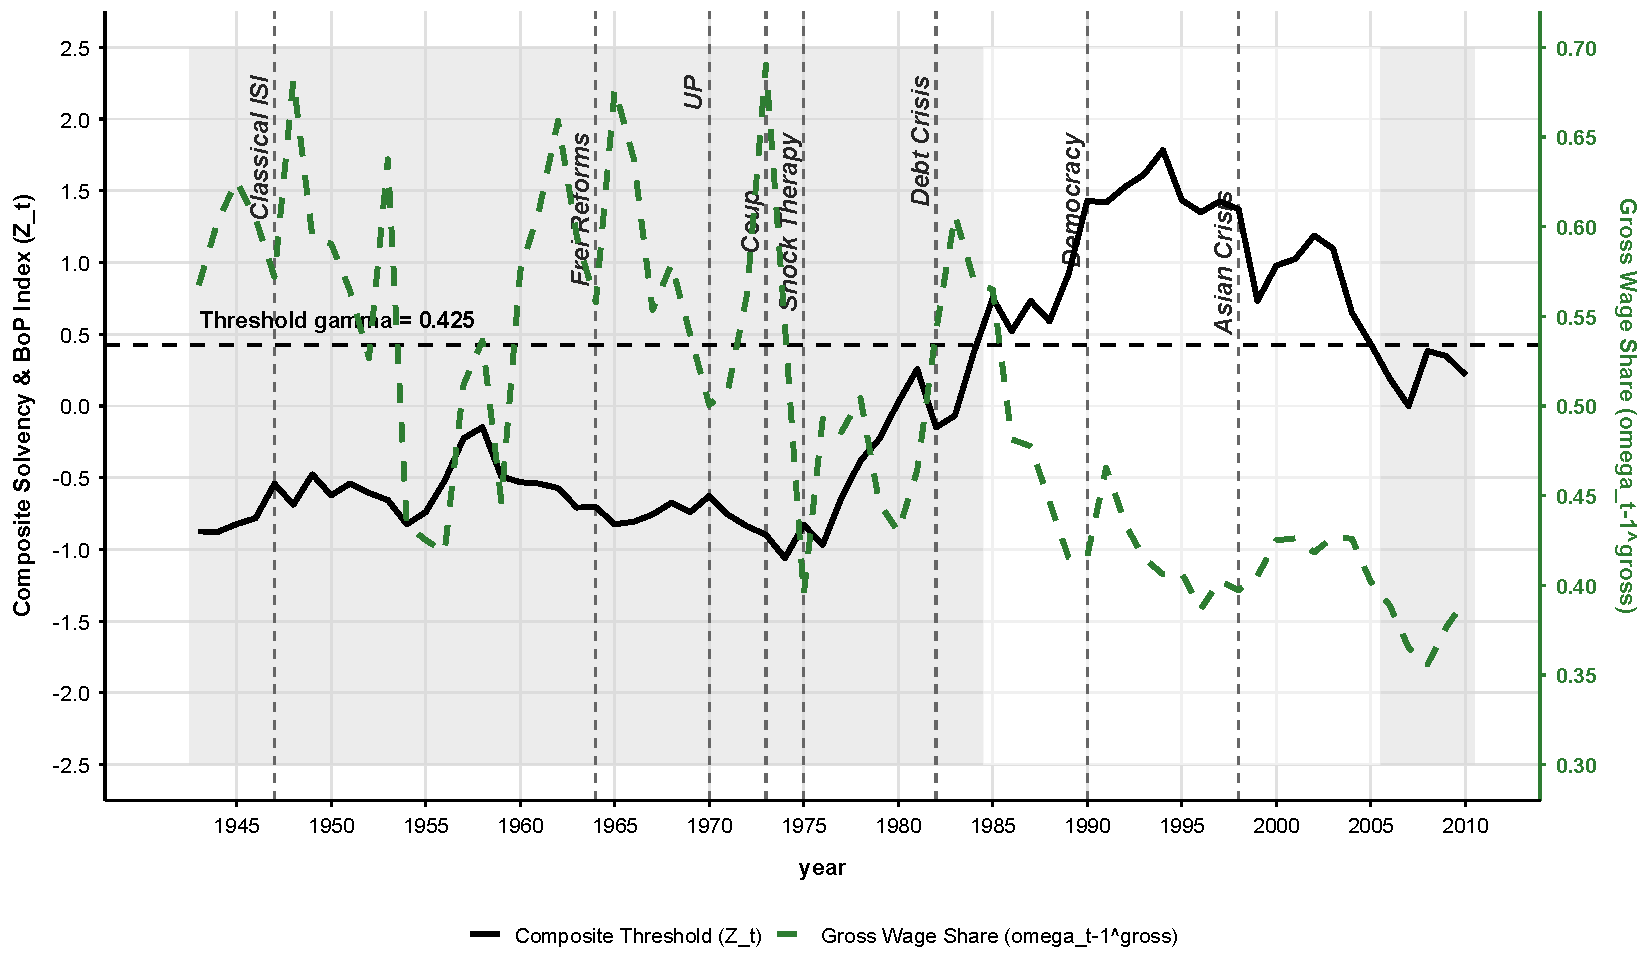
\includegraphics[width=0.95\textwidth]{figures/fig_cl_results_z_omega_drivers.pdf}
	\begin{tabular}{p{0.92\textwidth}}
		\footnotesize \textbf{Note:} Primary left axis (solid black line) tracks the composite balance-of-payments threshold variable $Z_t = 0.2 \tilde{M}_t + 0.8 \tilde{S}_t$, with the optimal threshold $\hat{\gamma} = 0.425$ marked by the horizontal dashed line. Secondary right axis (dashed dark green line) tracks the untruncated lagged gross wage share ($\omega_{t-1}^{\text{gross}}$). Background light gray shading marks binding balance-of-payments regimes ($Z_t \le 0.425$). Vertical dashed lines mark historical institutional breakpoints.
	\end{tabular}
\end{figure}

\FloatBarrier

Based on \citet{Ffrench2018} account on over-heating pre-debt crisis in 1982, I recover the order of magnitude for productive capacitieis from the recursion
\begin{equation}
	\ln Y_t^p = \ln Y_{t-1}^p + \theta_t^{\text{Agg}} \left( \ln K_t^{\text{tot}} - \ln K_{t-1}^{\text{tot}} \right), \quad Y_{1981}^p = Y_{1981} \implies \mu_{1981} = 1.00
	\label{eq:chile_yp_recursion}
\end{equation}
and divide realized GDP by it to obtain utilization.
Figure~\ref{fig:cl_results_dual_theta_mu} plots the two series on dual
axes and Figure~\ref{fig:cl_results_theta_standalone} the elasticity alone.
Five regimes organize the path, and the external constraint separates them.
The early CORFO expansion (1942--1946) combined postwar demand above normal
capacity ($\mu_{1946} = 1.12$) with slack foreign exchange and elasticities
near $0.85$. The ISI stop-go crises (1947--1957) reversed both: recurring
shortages forced stabilization cycles that pulled utilization to
$\mu_{1955} = 0.84$. The socialist transition (1970--1975) combined
redistribution with credit blockade, and utilization bottomed at $0.72$
after the 1975 shock therapy. The debt boom and crash (1975--1982) ran the
sequence in reverse, with inflows carrying utilization to the 1981 peak and
the crisis erasing it within a year ($\mu_{1982} = 0.68$). The recovery and
commodity super-cycle (1984--2010) absorbed idle capacity rather than
creating new capacity, holding $\mu_t$ between $0.85$ and $0.98$ through
1997. In four of the five regimes the turning point is external rather than
distributive, the asymmetry the threshold specification was built to detect.

\begin{figure}[H]
	\centering
	\caption{Chilean Capacity Utilization ($\mu_t$) and Aggregate Transformation Elasticity ($\theta_t^{\text{Agg}}$)}
	\label{fig:cl_results_dual_theta_mu}
	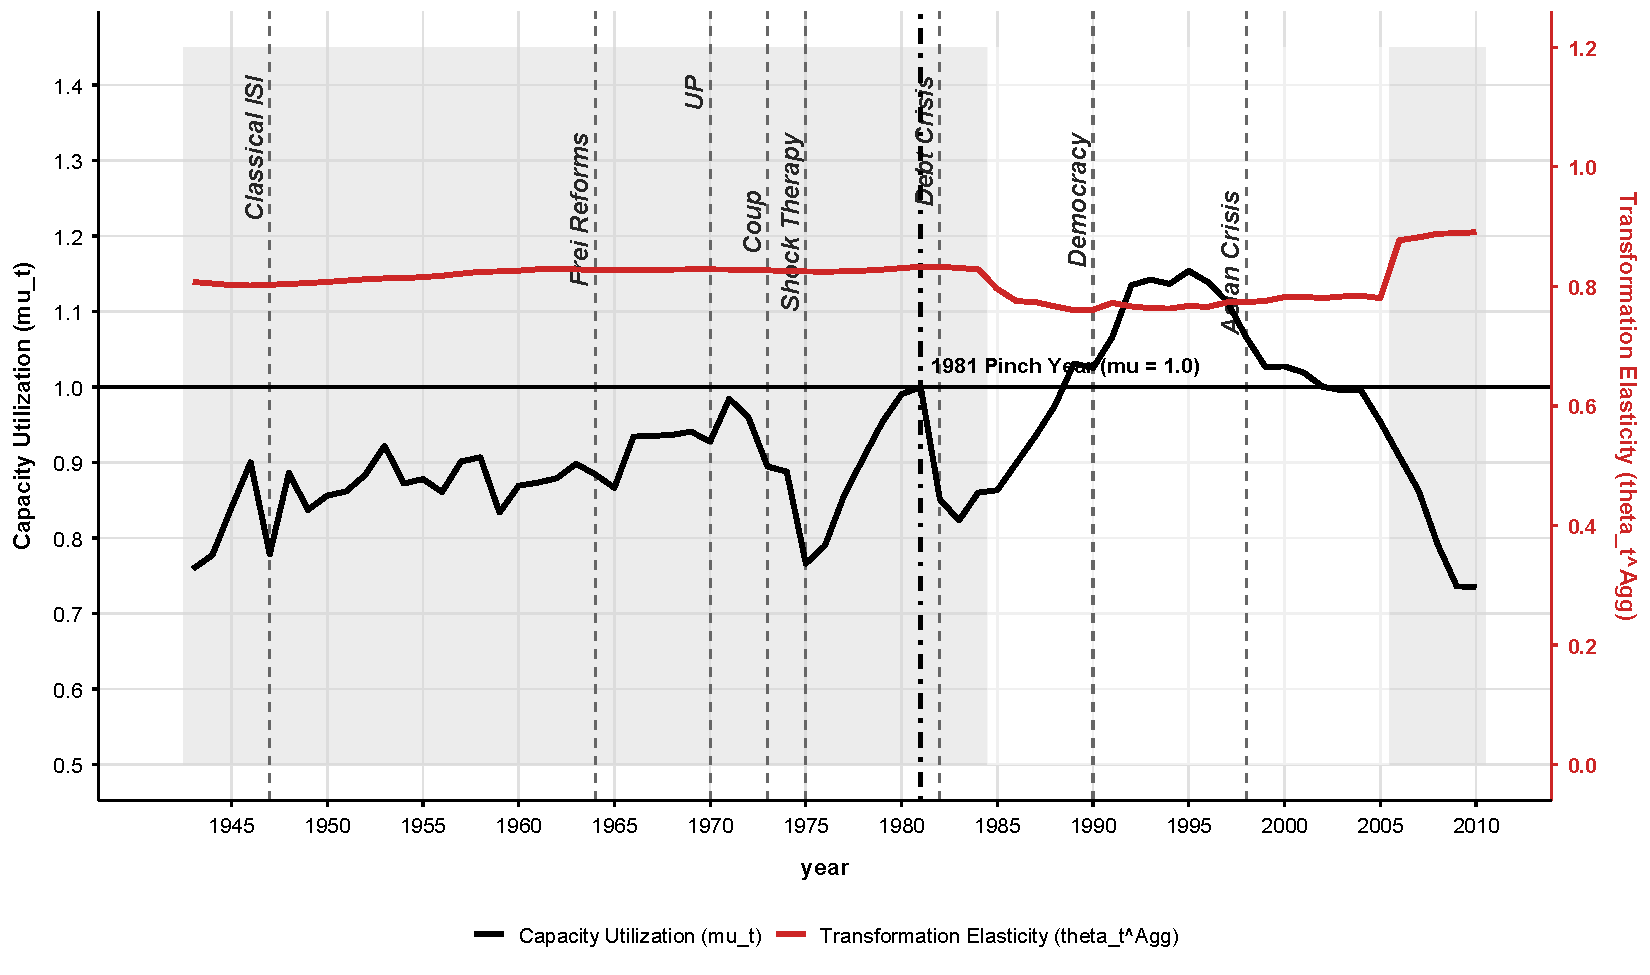
\includegraphics[width=0.95\textwidth]{figures/fig_cl_results_dual_theta_mu.pdf}
	\begin{tabular}{p{0.92\textwidth}}
		\footnotesize \textbf{Note:} Reconstructed capacity utilization rate $\mu_t$ (solid black line, left axis) anchored at the 1981 Ffrench-Davis pinch year ($\mu_{1981} = 1.00$) alongside the state-dependent aggregate transformation elasticity $\theta_t^{\text{Agg}}$ (solid firebrick line, right axis). Background light gray shading marks binding balance-of-payments regimes ($Z_t \le 0.425$). Vertical dashed lines mark institutional breakpoints.
	\end{tabular}
\end{figure}

\begin{figure}[H]
	\centering
	\caption{Standalone Chilean Aggregate Transformation Elasticity ($\theta_t^{\text{Agg}}$)}
	\label{fig:cl_results_theta_standalone}
	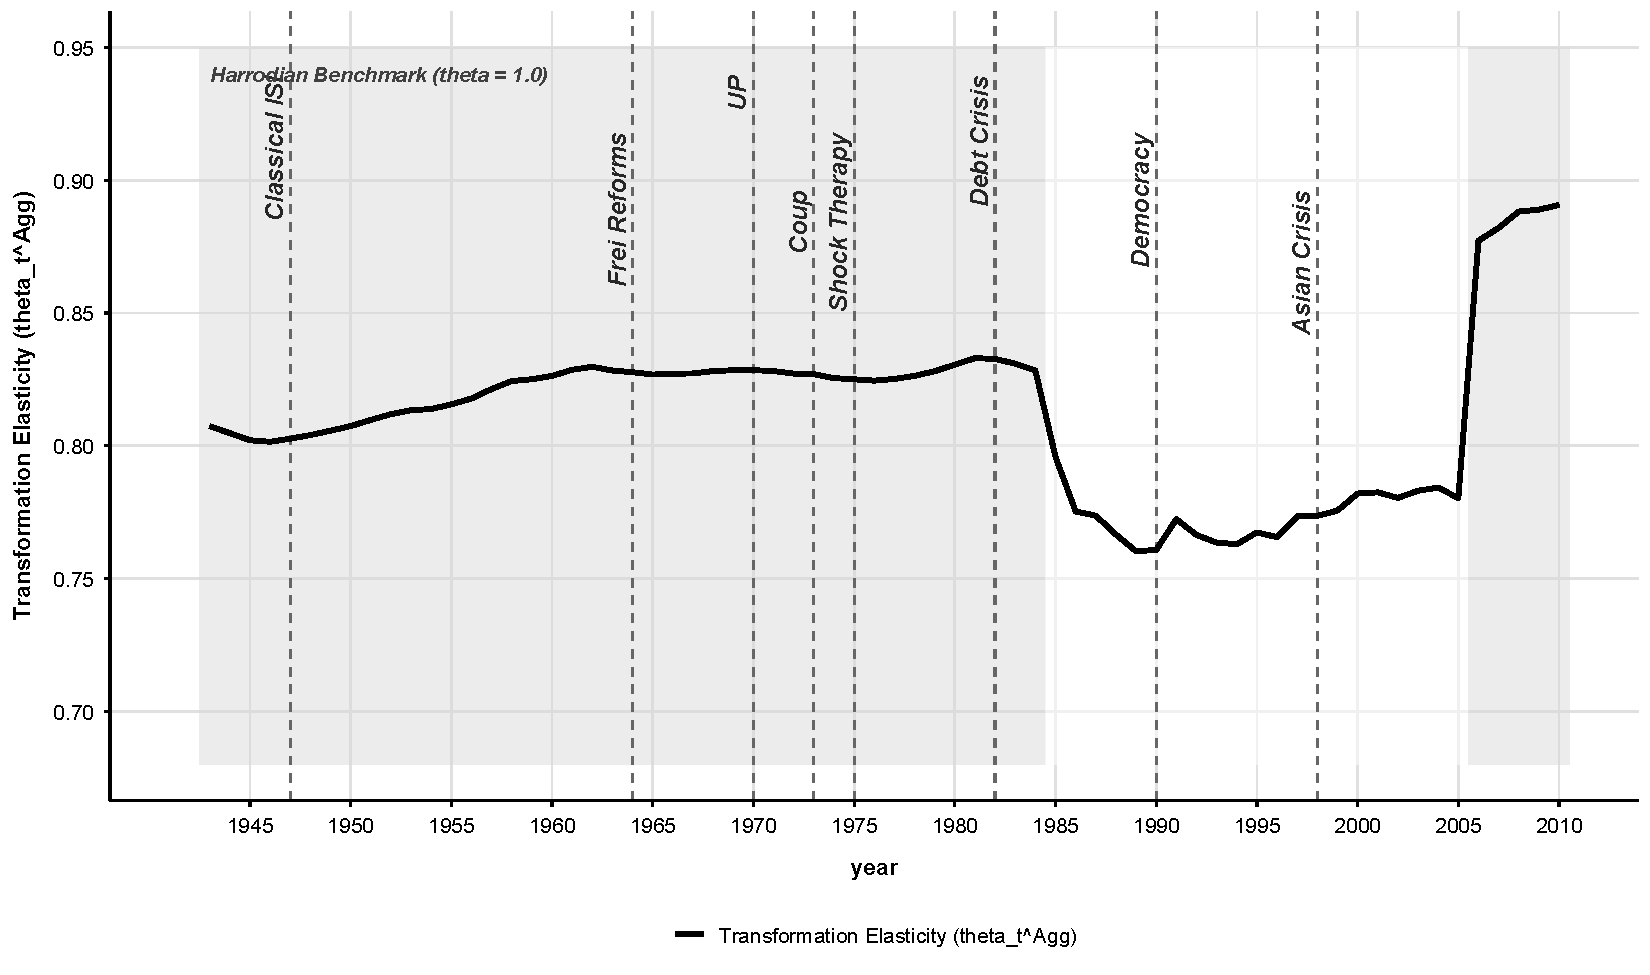
\includegraphics[width=0.95\textwidth]{figures/fig_cl_results_theta_standalone.pdf}
	\begin{tabular}{p{0.92\textwidth}}
		\footnotesize \textbf{Note:} Standalone trajectory of the aggregate transformation elasticity $\theta_t^{\text{Agg}}$ (solid firebrick line) on an uncompressed vertical scale ($0.68$ to $0.95$). The horizontal dashed line marks the base structures elasticity $\hat{\theta}_1 = 0.6970$. Background light gray shading marks binding balance-of-payments regimes ($Z_t \le 0.425$). Vertical dashed lines mark institutional breakpoints.
	\end{tabular}
\end{figure}

\FloatBarrier

Figure~\ref{fig:cl_results_z_components} decomposes the index into reserve
cover and import demand imbalances, and the two components show that the
constraint changes its institutional form across regimes. Under the fixed
and crawling pegs of the ISI period (1943--1973), reserve exhaustion forced
sharp devaluations and structural inflation \citep{Sunkel1958}, in line with
the periodization of \citet{Ffrench2002} and \citet{Ahumada2019}. Under the
post-2000 free float with inflation targeting, binding conditions produced
no runaway inflation; they produced extractivist re-primarization, real
appreciation, and profit repatriation by multinational mining
\citep{Palma2019, Ahumada2019}. Capital goods imports for extractive
projects, together with dividend outflows, truncated the conversion of
accumulation into broad-based domestic capacity.

\begin{figure}[H]
	\centering
	\caption{Decomposition of the Chilean External Constraint Index ($Z_t$ Components)}
	\label{fig:cl_results_z_components}
	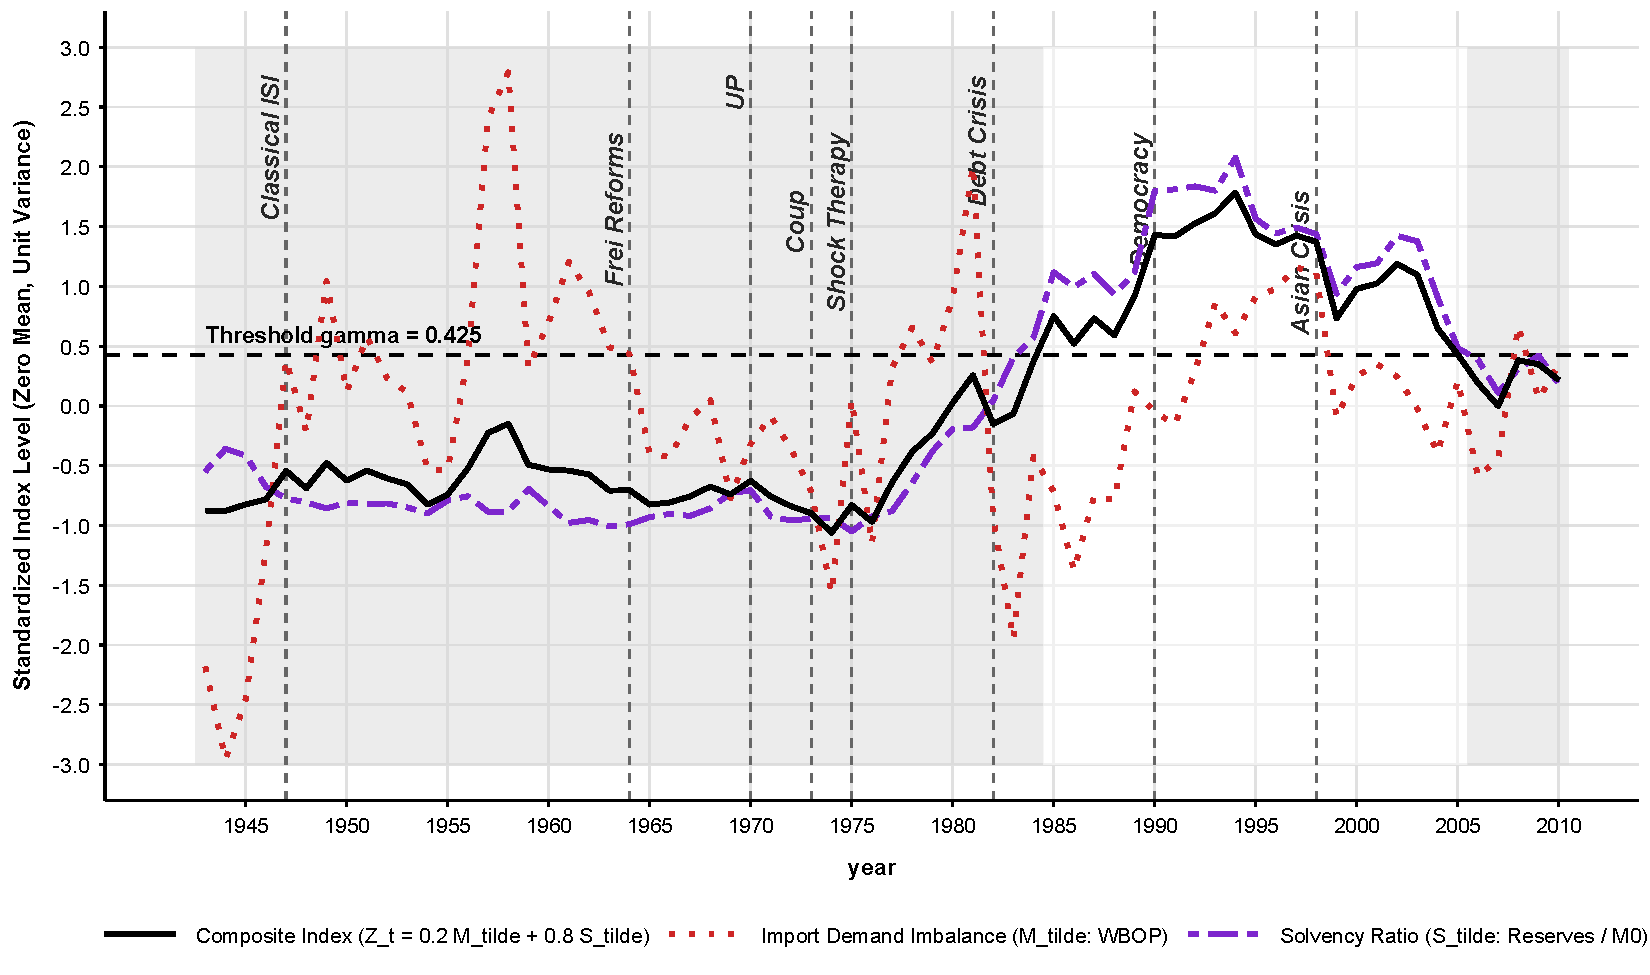
\includegraphics[width=0.95\textwidth]{figures/fig_cl_results_z_components.pdf}
	\begin{tabular}{p{0.92\textwidth}}
		\footnotesize \textbf{Note:} Decomposed ingredients of $Z_t = 0.2 \tilde{M}_t + 0.8 \tilde{S}_t$: standardized Central Bank solvency ratio $\tilde{S}_t$ (reserves to base money $M0$, purple twodash line), WBOP import demand imbalance $\tilde{M}_t$ (red dotted line, thickness 1.3), and composite index $Z_t$ (solid black line). Horizontal dashed line marks the threshold $\hat{\gamma} = 0.425$. Background light gray shading marks binding regimes ($Z_t \le 0.425$).
	\end{tabular}
\end{figure}

Two caveats qualify the reading of these regimes. The first concerns the
classifier. States are assigned by a single linear combination,
$Z_t = 0.2\tilde{M}_t + 0.8\tilde{S}_t$, with the weight and the threshold
chosen by grid search over the profile sum of squared residuals and a hard
cutoff at $\hat{\gamma} = 0.425$. This is a deterministic classification in
the sense of \citet{Hansen2000}, not a probabilistic regime model: there
are no transition probabilities and no persistence parameter, and after the
search $(\hat{p}, \hat{\gamma})$ enter the elasticity path as if known. The
simulation bounds charge for the threshold search but not for the weight
grid, so regime uncertainty is confined to the interval $[0.380, 0.472]$
and is not propagated into $\theta_t^{\text{Agg}}$. A Markov-switching or
smooth-transition extension would assign a binding probability to each year
and separate persistent shifts from transient bites; I leave that to future
work.

The second caveat concerns what the hard classification nonetheless
captures that a periodization cannot. $D_t^{\gamma}$ does not switch only
between the major regimes. Within the ISI era the index crosses the
threshold at the frequency of the stop-go cycle: import surges in the
expansion phase push it below the cutoff before the crisis, and post-crisis
stabilizations (devaluation, import compression, wage suppression) briefly
lift it back above. The 1998--99 tightening and the 2006--10 mining boom
are intra-cycle bites inside eras the conventional periodization labels
slack. The constraint operates at cycle frequency; the five regimes organize
the path at the lower frequency at which the institutional form of the
constraint changes, from inflation valve under administered exchange rates
to re-primarization valve under a free float. That double frequency is also
why the state-dependent indicator outperforms calendar breaks at 1987 or
1999: the breaks mark changes in the form, and the threshold tracks the
bites.

The center--periphery comparison follows. In the United States, where
capital equipment is produced domestically, wage pressure induces defensive
mechanization ($\hat{\theta}_1 < 0$, Section~4.3). In Chile, where machinery
must be imported, wage pressure induces mechanization
($\hat{\theta}_3 = +0.9583$) only while foreign exchange is unconstrained.
When reserves collapse, the constraint binds and truncates the choice of
technique. The distributive dividend that Okishio's viability condition
promises is not unavailable in principle in the periphery; it is unavailable
whenever the balance of payments binds.
